\part{Server}


\chapter{Overview}


一般来说,网络中的服务器对外提供服务,可以通过 Intranet 对内网提供服务,也可以通过 Internet 对外提供服务。

原始的通信网络中的电话和传真等设备的地位是对等的,但是用户和服务器的地位是不对等的,二者之间始终是发送请求和返回响应的关系。

P2P(peer-to-peer)对等网络中通过去中心化来实现了节点之间直接连接,并完成各自的连接认证、传输加密、数据压缩和数据校验等,因此P2P已经不同于客户端-服务器模型。

\begin{compactitem}
\item 对等网络要求通信双方必须同时在线;
\item 客户端-服务器模型要求服务器必须始终在线。
\end{compactitem}

软件服务器可以是管理资源并为用户提供服务的计算机软件,例如文件服务器(能使用户在其它计算机访问文件)、数据库服务器和应用程序服务器等,运行相关服务器软件的计算机就被称为硬件服务器,或主机(Host)。

最初,服务器通常是指具有较高计算能力,能够提供给多个用户使用的计算机,服务器软件工作在客户端-服务器或浏览器-服务器等模式下。


\begin{compactitem}
\item 文件服务器(File Server)或网络存储设备(Network Attached Storage);
\item 数据库服务器(Database Server),例如Oracle、MySQL、PostgreSQL和SQL Server 等;
\item 邮件服务器(Mail Server), 例如Sendmail、Postfix、Microsoft Exchange和Lotus Domino等;
\item 网页服务器(Web Server),例如httpd、IIS 和 nginx 等;
\item FTP 服务器(FTP Server),例如 vsftpd 和 Serv-U 等;
\item 域名服务器(DNS Server),例如BIND;
\item 应用程序服务器(Application Server),例如WebLogic、JBoss和GlassFish等;
\item 代理服务器(Proxy Server),例如Squid等。
\end{compactitem}


文件服务器可以为其他客户端提供文件检索和存储,通常具备某些特定的功能(例如磁盘镜像、多个网络接口等),后来文件服务器逐渐进化成带有 RAID 存储子系统和其他高可用特性的高性能存储系统。


在讨论主从式架构系统时,应用程序服务器区别于数据库服务器和文件服务器等,通常可以认为是运行Web应用程序的Web服务器。

具体来说,应用程序服务器是一种提供应用程序运行的环境的软件框架,可以为应用程序提供安全、数据、事务支持、负载平衡和分布式系统管理等服务。


网页服务器(Web server)可能是指用于网站的主机,也可能是指类似 httpd 的软件,运行在主机上并管理网页组件和回应网页浏览器的请求。例如,Redhat JBoss、Apache Tomcat和Oracle WebLogic等可以运行JSP的Web服务器都可以被认为是应用程序服务器。

每一个网页服务器至少会运行一个网页服务器程序,因此网页服务器也称为Web服务器,现在的Web服务器一般是指可以通过 HTTP 协议或 HTTPS 协议将 HTML 代码发送回客户端的主机,或者提供网页服务的服务器软件。

随着摩尔定律对于计算机硬件的影响和计算机软件的进化,服务器开始把越来越多的计算机任务放到客户端(例如Web浏览器)执行,这样服务器就可以专注于高性能计算和分布式计算等领域。



\section{C/S}



客户端-服务器(Client/Server)结构是一种把客户端与服务器区分开来的网络架构。例如,WWW就是客户端/服务器结构,服务器存储WWW资源,并响应客户端的请求。

\begin{compactitem}
\item 接受请求并进行特化处理的计算机称为服务器,可能会返回响应;
\item 发送请求并接受响应的计算机称为客户机,可能会丢失连接。
\end{compactitem}


每一个客户端软件的实例都可以向一个服务器或应用程序服务器发出请求。例如,当用户在Wikipedia.org阅读文章时,其主机和网页浏览器就被当做一个客户端,Wikipedia.org的主机、数据库和应用程序就被当做服务器。当网页浏览器向Wikipedia.org请求一个指定的文章时,Wikipedia.org的服务器从数据库中找出所有该文章需要的信息,并组合成一个网页,然后再发送回客户端的浏览器。

具体来说,服务端的特征可以包括:

\begin{compactitem}
\item 被动的角色(从)。
\item 等待来自用户端的请求。
\item 处理要求并传回结果。
\end{compactitem}

客户端的特征包括:

\begin{compactitem}
\item 主动的角色(主)。
\item 发送请求。
\item 等待直到收到回应,或退出。
\end{compactitem}

服务器可以是有状态或者无状态的。其中,无状态的服务器不会保留任何两个请求之间的信息,有状态服务器会记住请求之间的信息。

服务器与客户端之间的状态信息的作用域可以是全局的或者某个事务(session)的。例如,静态 HTML 页面服务器是一个无状态服务器的例子,而 Tomcat 是一个有状态服务器。



服务器端与客户端的交互可以使用循序图描述,循序图是 UML 中的一个标准。

点对点(peer-to-peer)架构不同于 C/S 架构,P2P网络上的每个使用端或程序的实体都拥有相同的等级,同时扮演客户端与服务器端的角色。





\section{B/S}

HTTP 是一个客户端终端和服务器端请求和应答的标准,其中定义了信息的传输格式化、如何被传输以及在各种命令下服务器和浏览器所采取的响应。

用户通过HTTP或者HTTPS协议请求的资源由URI(Uniform Resource Identifiers,统一资源标识符)来标识。

Web 服务器程序可以从网络接受 HTTP 请求并进行处理,然后提供 HTTP 回复给请求者,不过根据Web服务器的类型不同,其内部操作也有很大差别。

\begin{compactitem}
\item 客户端浏览器、网络爬虫或者其它的工具发起HTTP请求到服务器上指定端口(默认端口为 80),可以将客户端看作是用户的代理程序(user agent)。
\item HTTP 回复一般包含一个 HTML 文件,也可以包含纯文本文件、图像或其他类型的文件。
\end{compactitem}




一般来说,文件(例如HTML、文本或图像等)都存储在 Web 服务器的本地文件系统中,并且 URL(Uniform Resource Locator) 和本地文件名都有对应的组织结构,因此服务器可以简单的把 URL 映射到本地文件系统中,并且可以指定一个本地路径名为根目录。

Web 服务器上可以用来存储一些资源(例如 HTML 文件和图像),因此也可以将 Web 服务器称为源服务器(origin server),而且在用户代理和源服务器中间可能存在多个“中间层”(例如代理、网关或者隧道(tunnel))。

客户端访问静态Web服务器(或静态网站)时,根据用户的选择将会返回相应的静态页面。例如,在 example.test.com 服务器上安装了服务器软件,并把服务器软件的根目录指定为/home/public/web/,当一个浏览者输入 http://example.test.com/lips/index.html时,就可以指定example.test.com的服务器软件读取/home/public/web/lips/index.html 文件。



默认情况下,Web 服务器的根目录为/var/www/html 或/src/www,例如 CentOS 默认的网站根目录为/var/www/html。如果需要自定义网站根目录,可以在修改 httpd.conf 中的DocumentRoot 参数,而且务必开放权限让 Web 服务器(例如 httpd、Nginix、Lightttpd)的用户可以浏览网站根目录。




Web服务器也可以提供动态内容,而且动态内容可以是该服务器本身提供的功能或者可借助外挂模块实现的功能。例如,通过动态网站技术生成的网页都称为动态网页,服务器端程序根据客户端请求来返回相应的结果。

动态网站技术可以通过查询字符串等参数并配合HTTP方法来实现更多的功能,而且动态网页并不是独立保存在服务器上的网页文件,只有当用户向服务器发送请求时才会组合相关组件并返回一个完整的网页。

\begin{compactitem}
\item 用户注册
\item 用户登录
\item 在线调查
\item 用户管理
\item 订单管理
\end{compactitem}

用户可以使用静态语言或动态语言来创建网站,动态语言不需要任何预先处理就可以快速反馈结果,而且动态语言引擎可以作为Web服务器的一部分来运行代码,不需要调用外部程序,这样Web服务器就不需要承担任何额外的负担。

例如,PHP应用程序可以检查请求的URI或其他信息来确定需要执行的操作,并且根据需要来从数据库中检索信息,然后将这些信息通过HTML组合成相应网页,最后将结果返回给客户端浏览器。当用户在浏览器中持续操作时,每次请求都会触发上述完整的过程被重复执行,并且当多个用户访问动态网站时,Web服务器会进行并发处理。

\begin{center}
HTML+运算结果=最终网页
\end{center}

Web浏览器实现的动态处理功能可以让浏览器在处理HTML或XML的同时显示图像或动画等,而且浏览器可以处理并执行从Web服务器获得的脚本或其他多媒体信息。

默认情况下,Web浏览器除了发送请求、接收响应和渲染输出之外功能有限,不过通过其内置的脚本引擎(例如Google V8引擎)或第三方插件等可以实现和操作系统相应的动态处理功能。



\begin{compactitem}
\item Adobe Flash Player可以让浏览器播放flash动画;
\item Apple Quicktime Player可以让浏览器播放mov视频;
\item Mozilla PDF.js可以让浏览器在线打开PDF文档。
\end{compactitem}


\section{Mechanism}


\subsection{epoll}

epoll is a Linux kernel system call, a scalable I/O event notification mechanism, first introduced in Linux kernel 2.5.44. It is meant to replace the older POSIX select(2) and poll(2) system calls, to achieve better performance in more demanding applications, where the number of watched file descriptors is large (unlike the older system calls, which operate in O(n) time, epoll operates in O(1) time). 

epoll is similar to FreeBSD's kqueue, in that it operates on a configurable kernel object, exposed to user space as a file descriptor of its own.


\begin{lstlisting}[language=PHP]
int epoll_create1(int flags);
\end{lstlisting}

Creates an epoll object and returns its file descriptor. The flags parameter allows epoll behavior to be modified. It has only one valid value, EPOLL\_CLOEXEC. epoll\_create() is an older variant of epoll\_create1() and is deprecated as of Linux kernel version 2.6.27 and glibc version 2.9.




\begin{lstlisting}[language=PHP]
int epoll_ctl(int epfd, int op, int fd, struct epoll_event *event);
\end{lstlisting}

Controls (configures) which file descriptors are watched by this object, and for which events. op can be ADD, MODIFY or DELETE.





\begin{lstlisting}[language=PHP]
int epoll_wait(int epfd, struct epoll_event *events, int maxevents, int timeout);
\end{lstlisting}

Waits for any of the events registered for with epoll_ctl, until at least one occurs or the timeout elapses. Returns the occurred events in events, up to maxevents at once.

epoll provides both edge-triggered and level-triggered modes. In edge-triggered mode, a call to epoll\_wait will return only when a new event is enqueued with the epoll object, while in level-triggered mode, epoll\_wait will return as long as the condition holds.

For instance, if a pipe, registered with epoll, has received data, a call to epoll\_wait will return, signaling the presence of data to be read. Suppose the reader only consumed part of data from the buffer. In level-triggered mode, further calls to epoll\_wait will return immediately, as long as the pipe's buffer contains data to be read. In edge-triggered mode, however, epoll\_wait will return only once new data is written to the pipe.



\subsection{select}

select is a system call and application programming interface (API) in Unix-like and POSIX-compliant operating systems for examining the status of file descriptors of open input/output channels. The select system call is similar to the poll facility introduced in UNIX System V and later operating systems.

In the C programming language, the select system call is declared in the header file sys/select.h or unistd.h, and has the following syntax:

\begin{lstlisting}[language=PHP]
int select(int nfds, fd_set *readfds, fd_set *writefds, fd_set *errorfds, struct timeval *timeout);
\end{lstlisting}



\begin{longtable}{|m{40pt}|m{350pt}|}
%head
\multicolumn{2}{r}{}
\tabularnewline\hline
argument&description
\endhead
%endhead

%firsthead
\caption{select(UNIX)}\\
\hline
argument&description
\endfirsthead
%endfirsthead

%foot
\multicolumn{2}{r}{}
\endfoot
%endfoot

%lastfoot
\endlastfoot
%endlastfoot

\hline
nfds	&This is an integer one more than the maximum of any file descriptor in any of the sets. In other words, while adding file descriptors to each of the sets, you must calculate the maximum integer value of all of them, then increment this value by one, and then pass this as nfds.\\
\hline
readfds&	fd\_set type holding the file descriptors to be checked for being ready to read, and on output indicates which file descriptors are ready to read. Can be NULL.\\
\hline
writefds&	fd\_set type holding the file descriptors to be checked for being ready to write, and on output indicates which file descriptors are ready to write. Can be NULL.\\
\hline
errorfds&	fd\_set type holding the file descriptors to be checked for error conditions pending, and on output indicates which file descriptors have error conditions pending. Can be NULL.\\
\hline
timeout&	structure of type struct timeval that specifies a maximum interval to wait for the selection to complete. If the timeout argument points to an object of type struct timeval whose members are 0, select() does not block. If the timeout argument is NULL, select() blocks until an event causes one of the masks to be returned with a valid (non-zero) value. Linux will update the timeout in place to indicate how much time was elapsed, though this behavior is not shared by most other Unix systems.\\
\hline
\end{longtable}

fd\_set type arguments may be manipulated with four utility macros: FD\_SET(), FD\_CLR(), FD\_ZERO(), and FD\_ISSET().

Select returns the total number of bits set in readfds, writefds and errorfds, or zero if the timeout expired, and -1 on error.

The sets of file descriptor used in select are finite in size, depending on the operating system. The newer system call poll provides a more flexible solution.


\begin{lstlisting}[language=PHP]
#include <stdio.h>
#include <stdlib.h>
#include <string.h>

#include <sys/types.h>
#include <sys/socket.h>
#include <netinet/in.h>
#include <netdb.h>

#include <sys/select.h>
#include <fcntl.h>
#include <unistd.h>
#include <err.h>
#include <errno.h>

#define PORT "9421"

/* function prototypes */
void die(const char*);

int main(int argc, char **argv)
{
    int sockfd, new, maxfd, on = 1, nready, i;

    struct addrinfo *res0, *res, hints;

    char buffer[BUFSIZ];

    fd_set master, readfds;

    int error;

    ssize_t nbytes;

    (void)memset(&hints, '\0', sizeof(struct addrinfo));

    hints.ai_family = AF_INET;
    hints.ai_socktype = SOCK_STREAM;
    hints.ai_protocol = IPPROTO_TCP;
    hints.ai_flags = AI_PASSIVE;

    if (0 != (error = getaddrinfo(NULL, PORT, &hints, &res0)))
        errx(EXIT_FAILURE, "%s", gai_strerror(error));

    for (res = res0; res; res = res->ai_next)
    {
        if (-1 == (sockfd = socket(res->ai_family, res->ai_socktype, res->ai_protocol)))
        {
            perror("socket()");
            continue;
        }

        if (-1 == (setsockopt(sockfd, SOL_SOCKET, SO_REUSEADDR, (char*)&on, sizeof(int))))
        {
            perror("setsockopt()");
            continue;
        }

        if (-1 == (bind(sockfd, res->ai_addr, res->ai_addrlen)))
        {
            perror("bind");
            continue;
        }

        break;

    }

    if (-1 == sockfd)
        exit(EXIT_FAILURE);

    freeaddrinfo(res0);

    if (-1 == (listen(sockfd, 32)))
        die("listen()");

    if (-1 == (fcntl(sockfd, F_SETFD, O_NONBLOCK)))
        die("fcntl()");

    FD_ZERO(&master);
    FD_ZERO(&readfds);

    FD_SET(sockfd, &master);

    maxfd = sockfd;

    while (1)
    {
        memcpy(&readfds, &master, sizeof(master));

        (void)printf("running select()\n");

        if (-1 == (nready = select(maxfd+1, &readfds, NULL, NULL, NULL)))
            die("select()");

        (void)printf("Number of ready descriptor: %d\n", nready);

        for (i=0; i<=maxfd && nready>0; i++)
        {
            if (FD_ISSET(i, &readfds))
            {
                nready--;

                if (i == sockfd)
                {
                    (void)printf("Trying to accept() new connection(s)\n");

                    if (-1 == (new = accept(sockfd, NULL, NULL)))
                    {
                        if (EWOULDBLOCK != errno)
                            die("accept()");

                        break;
                    }

                    else
                    {

                        if (-1 == (fcntl(new, F_SETFD, O_NONBLOCK)))
                            die("fcntl()");

                        FD_SET(new, &master);

                        if (maxfd < new)
                            maxfd = new;
                    }
                }

                else
                {
                    (void)printf("recv() data from one of descriptors(s)\n");

                    nbytes = recv(i, buffer, sizeof(buffer), 0);
                    if (nbytes <= 0)
                    {
                        if (EWOULDBLOCK != errno)
                            die("recv()");

                        break;
                    }

                    buffer[nbytes] = '\0';
                    printf("%s", buffer);

                    (void)printf("%zi bytes received.\n", nbytes);

                    close(i);
                    FD_CLR(i, &master);

                }
            }

        }

    }
    return 0;
}

void die(const char *msg)
{
    perror(msg);
    exit(EXIT_FAILURE);
}
\end{lstlisting}




\begin{lstlisting}[language=PHP]

\end{lstlisting}




\begin{lstlisting}[language=PHP]

\end{lstlisting}






\begin{lstlisting}[language=PHP]

\end{lstlisting}




\begin{lstlisting}[language=PHP]

\end{lstlisting}



\subsection{kqueue}



Kqueue is a scalable event notification interface introduced in FreeBSD 4.1, also supported in NetBSD, OpenBSD, DragonflyBSD, and OS X. Kqueue was originally authored in 2000 by Jonathan Lemon, then involved with the FreeBSD Core Team.

Kqueue provides efficient input and output event pipelines between the kernel and userland. Thus, it is possible to modify event filters as well as receive pending events while using only a single system call to kevent(2) per main event loop iteration. This contrasts with older traditional polling system calls such as poll(2) and select(2) which are less efficient, especially when polling for events on a large number of file descriptors.

Kqueue not only handles file descriptor events but is also used for various other notifications such as file modification monitoring, signals, asynchronous I/O events (AIO), child process state change monitoring and timers which support nanosecond resolution.

Some other operating systems which traditionally only supported select(2) and poll(2) also currently provide more efficient polling alternatives, such as epoll on Linux and I/O Completion Ports on Windows and Solaris.

Kqueue (or related techniques) provides the foundation for scalable event-driven I/O architectures such as Node.js in the web server space.

The following is a telnet-like program that reads a message from standard input and then writes it to a network socket. At the same time, it reads from the other end of network socket and prints it out to the standard output.

\begin{lstlisting}[language=PHP]
#include <stdio.h>
#include <stdlib.h>
#include <string.h>
 
#include <sys/types.h>
#include <sys/socket.h>
#include <netdb.h>
#include <fcntl.h>
#include <unistd.h>
#include <sys/event.h>
#include <sys/time.h>
#include <err.h>
#include <errno.h>
 
void die(const char*);
int make_nonblocking(int);
 
int main(int argc, char *argv[])
{
	int sockfd, nev, kq; 
	struct addrinfo hints, *res, *res0; 
	struct kevent change[2], event[2]; 
	ssize_t nbytes;	
	int error; 
	char buf[BUFSIZ]; 
	const char *cause = NULL;
 
	if (3 != argc)
	{
		fprintf(stderr, "Usage: %s address port\n", argv[0]);
		exit(EXIT_FAILURE);
	}
 
	(void)memset(&hints, '\0', sizeof(struct addrinfo));
 
	hints.ai_family = AF_INET;
	hints.ai_socktype = SOCK_STREAM;
 
	if (0 != (error = getaddrinfo(argv[1], argv[2], &hints, &res0)))
		errx(EXIT_FAILURE, "%s", gai_strerror(error));
 
	sockfd = -1;
 
	for (res = res0; res; res = res->ai_next)
	{
		if (-1 == (sockfd = socket(res->ai_family, res->ai_socktype,
		 res->ai_protocol)))
		{
			cause = "socket";
			continue;
		}
 
		if (-1 == connect(sockfd, res->ai_addr, res->ai_addrlen))
		{
			cause = "connect()";
			close(sockfd);
			sockfd = -1;
			continue;
		}

		break;
		/* NOTREACHED */
 
	}
 
	if (-1 == sockfd)
		die(cause);
		
	freeaddrinfo(res0);
 
	if (-1 == make_nonblocking(sockfd))
		die("make_nonblock()");
 
	if (-1 == make_nonblocking(STDIN_FILENO))
		die("make_nonblock()");
 
	if (-1 == (kq = kqueue()))
		die("kqueue()");
 
	EV_SET(&change[0], STDIN_FILENO, EVFILT_READ, EV_ADD | EV_ENABLE,0, 0, 0);
	EV_SET(&change[1], sockfd, EVFILT_READ, EV_ADD | EV_ENABLE,0, 0, 0);
	 
	 if (-1 == kevent(kq, change, 2, NULL, 0, NULL))
	 	die("kevent()");
 
	for (;;)
	{
		printf("blocking in kevent()\n");
		if (-1 == (nev = kevent(kq, NULL, 0, event, 2, NULL)))
			die("kevent()");		
		printf("kevent() returned %d\n", nev); 
		
		for (int i = 0; i < nev; i++)
		{
			if (event[i].ident == STDIN_FILENO)
			{
				fgets(buf, sizeof(buf), stdin);
				nbytes = send(sockfd, buf, strlen(buf), 0);
				if (-1 == nbytes)
					if (EWOULDBLOCK != errno)
						die("send()");
 
			}
			else
			{
				while ((nbytes = recv(sockfd, buf, sizeof(buf), 0)) > 0)
				{					
					if (nbytes != write(STDOUT_FILENO, buf, nbytes))
					{
						die("write()");
					}
				}
 
				if (-1 == nbytes)
				{
					if (EWOULDBLOCK != errno)
						die("recv()");
				}
				else if (EV_EOF & event[i].flags)
				{
					printf("the peer has closed the connection, exiting...\n");
					exit(0);
				}				
			} 
		} 
	} 
	return 0;
}
 
void die(const char *str)
{
	perror(str);
	exit(EXIT_FAILURE);
}

int make_nonblocking(int fd)
{
	int flags;
	if (-1 == (flags = fcntl(fd, F_GETFL)))
		return -1;
	
	flags |= O_NONBLOCK;
	
	if (-1 == fcntl(fd, F_SETFL, flags))
		return -1;
	
	return 0;	
}
\end{lstlisting}

OS-independent libraries with good support for kqueue:

\begin{compactitem}
\item libevent
\item libuv
\end{compactitem}

Kqueue equivalent for other platforms:

\begin{compactitem}
\item on Linux: epoll
\item on Solaris, Windows and AIX: I/O Completion Ports
\end{compactitem}




\begin{lstlisting}[language=PHP]

\end{lstlisting}






\begin{lstlisting}[language=PHP]

\end{lstlisting}




\begin{lstlisting}[language=PHP]

\end{lstlisting}





\chapter{LAMP}


Linux、Apache、MySQL和PHP等开放源代码程序本身并不是专门设计成同其他程序协同工作的,但是由于它们的廉价和普遍,LAMP组合才开始流行并被大多数Linux发行版本进行了捆绑发行。


在LAMP中的软件被合理地使用时,它们地表现类似一个具有活力的“解决方案包”(Solution Packages)。

最初,LAMP的脚本组件中包括了使用Perl实现地CGI Web接口,可以允许网页浏览器的用户在服务器上执行一个程序,并且和接受静态的内容一样接受动态的内容。

脚本语言(例如Perl、PHP和Python等)可以有效地操作文本流,因此被开发者引入来创建Web服务器上的外部程序。

从RHEL/CentOS 7开始已经不再內置MySQL并改用MariaDB,不过MariaDB和MySQL的使用方式相同,原来的MySQL数据库也可以直接升級使用。


\section{Apache}

\subsection{Compile}

下载源代码(httpd-2.4.16),并以默认配置来编译安装Apache。

\begin{lstlisting}[language=bash]
$ cd ~
$ mkdir src
$ cd src
$ wget http://mirrors.aliyun.com/apache/httpd/httpd-2.4.16.tar.gz
--2015-08-11 22:47:46--  http://mirrors.aliyun.com/apache/httpd/httpd-2.4.16.tar.gz
Resolving mirrors.aliyun.com (mirrors.aliyun.com)... 115.28.122.210, 112.124.140.210
Connecting to mirrors.aliyun.com (mirrors.aliyun.com)|115.28.122.210|:80... connected.
HTTP request sent, awaiting response... 200 OK
Length: 6899517 (6.6M) [application/octet-stream]
Saving to: ‘httpd-2.4.16.tar.gz’

httpd-2.4.16.tar.gz  100%[================>]  6.58M  1.00MB/s  in 7.3s   

2015-08-11 22:47:53 (918 KB/s) -‘httpd-2.4.16.tar.gz’ saved [6899517/6899517]
$ tar zxvf httpd-2.4.16.tar.gz
httpd-2.4.16/
httpd-2.4.16/.deps
httpd-2.4.16/.gdbinit
httpd-2.4.16/ABOUT_APACHE
httpd-2.4.16/acinclude.m4
httpd-2.4.16/ap.d
httpd-2.4.16/Apache-apr2.dsw
httpd-2.4.16/Apache.dsw
httpd-2.4.16/apache_probes.d
httpd-2.4.16/build/
httpd-2.4.16/BuildAll.dsp
httpd-2.4.16/BuildBin.dsp
httpd-2.4.16/buildconf
httpd-2.4.16/CHANGES
httpd-2.4.16/CMakeLists.txt
httpd-2.4.16/config.layout
httpd-2.4.16/configure
httpd-2.4.16/configure.in
httpd-2.4.16/docs/
httpd-2.4.16/emacs-style
httpd-2.4.16/httpd.dsp
httpd-2.4.16/httpd.spec
httpd-2.4.16/include/
httpd-2.4.16/INSTALL
httpd-2.4.16/InstallBin.dsp
httpd-2.4.16/LAYOUT
httpd-2.4.16/libhttpd.dsp
httpd-2.4.16/LICENSE
httpd-2.4.16/Makefile.in
httpd-2.4.16/Makefile.win
httpd-2.4.16/modules/
httpd-2.4.16/NOTICE
httpd-2.4.16/NWGNUmakefile
httpd-2.4.16/os/
httpd-2.4.16/README
httpd-2.4.16/README.cmake
httpd-2.4.16/README.platforms
httpd-2.4.16/ROADMAP
httpd-2.4.16/server/
httpd-2.4.16/srclib/
httpd-2.4.16/support/
httpd-2.4.16/test/
httpd-2.4.16/VERSIONING
httpd-2.4.16/test/.indent.pro
httpd-2.4.16/test/check_chunked
...
httpd-2.4.16/test/time-sem.c
httpd-2.4.16/support/.indent.pro
...
httpd-2.4.16/support/SHA1/README.sha1
httpd-2.4.16/srclib/Makefile.in
httpd-2.4.16/server/.indent.pro
...
httpd-2.4.16/server/mpm/event/mpm_default.h
httpd-2.4.16/os/.indent.pro
...
httpd-2.4.16/os/bs2000/os.h
httpd-2.4.16/modules/aaa/
...
httpd-2.4.16/modules/aaa/NWGNUmakefile
httpd-2.4.16/include/.indent.pro
...
httpd-2.4.16/include/util_xml.h
httpd-2.4.16/docs/cgi-examples/
...
httpd-2.4.16/docs/cgi-examples/test-cgi
httpd-2.4.16/build/aix/
...
httpd-2.4.16/build/aix/README
\end{lstlisting}

configure脚本

\begin{lstlisting}[language=bash]
$ cd src/httpd-2.4.16
$ ./configure
checking for chosen layout... Apache
checking for working mkdir -p... yes
checking for grep that handles long lines and -e... /usr/bin/grep
checking for egrep... /usr/bin/grep -E
checking build system type... x86_64-unknown-linux-gnu
checking host system type... x86_64-unknown-linux-gnu
checking target system type... x86_64-unknown-linux-gnu
configure: 
configure: Configuring Apache Portable Runtime library...
configure: 
checking for APR... no
configure: error: APR not found.  Please read the documentation.
\end{lstlisting}


\subsection{Dependence}


解决依赖关系

APR(Apache Portable Run-time Libraries)主要为上层的应用程序提供一个可以跨越多操作系统平台使用的底层支持接口库,其对于Tomcat最大的作用就是socket调度。例如,在慢速网络上(模拟Internet)将Tomcat线程数开到300以上,然后模拟大量的并发请求时没有APR,基本上300个线程很快就会用满,以后的请求就只好等待,在安装APR之后,并发的线程数量明显下降,从原来的300可能会马上下降到只有几十,这样新的请求会毫无阻塞的进来。

在早期的Apache版本中,应用程序本身必须能够处理各种具体操作系统平台的细节,并针对不同的平台调用不同的处理函数。随着Apache的进一步开发,Apache组织决定将这些通用的函数独立出来并发展成为一个新的项目,这样APR的开发就从Apache中独立出来,Apache仅仅是使用APR而已。

虽然在局域网进行本地测试时,高并发的情况也可以被很容易的处理,但是在真实的Internet环境下,页面处理时间只占0.1\%都不到,绝大部分时间都用来页面传输。如果不用APR,一个线程同一时间只能处理一个用户,势必会造成阻塞,所以生产环境下使用APR是非常必要的。

一般情况下,APR开发包很容易理解为仅仅是一个开发包,不过事实上并不是。目前,完整的APR实际上包含了三个开发包:apr、apr-util以及apr-iconv,每一个开发包分别独立开发,并拥有自己的版本。

\begin{lstlisting}[language=bash]
$ cd ~/src
$ wget http://mirrors.aliyun.com/apache/apr/apr-1.5.2.tar.gz
--2015-08-11 23:02:52--  http://mirrors.aliyun.com/apache/apr/apr-1.5.2.tar.gz
Resolving mirrors.aliyun.com (mirrors.aliyun.com)... 115.28.122.210, 112.124.140.210
Connecting to mirrors.aliyun.com (mirrors.aliyun.com)|115.28.122.210|:80... connected.
HTTP request sent, awaiting response... 200 OK
Length: 1031613 (1007K) [application/octet-stream]
Saving to: ‘apr-1.5.2.tar.gz’

apr-1.5.2.tar.gz  100%[======================>]  1007K  898KB/s  in 1.1s   

2015-08-11 23:02:53 (898 KB/s) - ‘apr-1.5.2.tar.gz’ saved [1031613/1031613]
$ cd ~/apr-1.5.2
$ ./configure
$ make
$ sudo make install
[sudo] password for test: 
make[1]: Entering directory '/home/test/src/apr-1.5.2'
make[1]: Nothing to be done for 'local-all'.
make[1]: Leaving directory '/home/test/src/apr-1.5.2'
/home/test/src/apr-1.5.2/build/mkdir.sh /usr/local/apr/lib /usr/local/apr/bin /usr/local/apr/build-1 \
	     /usr/local/apr/lib/pkgconfig /usr/local/apr/include/apr-1
mkdir /usr/local/apr
mkdir /usr/local/apr/lib
mkdir /usr/local/apr/bin
mkdir /usr/local/apr/build-1
mkdir /usr/local/apr/lib/pkgconfig
mkdir /usr/local/apr/include
mkdir /usr/local/apr/include/apr-1
/usr/bin/install -c -m 644 /home/test/src/apr-1.5.2/include/apr.h /usr/local/apr/include/apr-1
for f in /home/test/src/apr-1.5.2/include/apr_*.h; do \
    /usr/bin/install -c -m 644 ${f} /usr/local/apr/include/apr-1; \
done
/bin/sh /home/test/src/apr-1.5.2/libtool --mode=install /usr/bin/install -c -m 755 libapr-1.la /usr/local/apr/lib
libtool: install: /usr/bin/install -c -m 755 .libs/libapr-1.so.0.5.2 /usr/local/apr/lib/libapr-1.so.0.5.2
libtool: install: (cd /usr/local/apr/lib && { ln -s -f libapr-1.so.0.5.2 libapr-1.so.0 || { rm -f libapr-1.so.0 && ln -s libapr-1.so.0.5.2 libapr-1.so.0; }; })
libtool: install: (cd /usr/local/apr/lib && { ln -s -f libapr-1.so.0.5.2 libapr-1.so || { rm -f libapr-1.so && ln -s libapr-1.so.0.5.2 libapr-1.so; }; })
libtool: install: /usr/bin/install -c -m 755 .libs/libapr-1.lai /usr/local/apr/lib/libapr-1.la
libtool: install: /usr/bin/install -c -m 755 .libs/libapr-1.a /usr/local/apr/lib/libapr-1.a
libtool: install: chmod 644 /usr/local/apr/lib/libapr-1.a
libtool: install: ranlib /usr/local/apr/lib/libapr-1.a
libtool: finish: PATH="/sbin:/bin:/usr/sbin:/usr/bin:/sbin" ldconfig -n /usr/local/apr/lib
----------------------------------------------------------------------
Libraries have been installed in:
   /usr/local/apr/lib

If you ever happen to want to link against installed libraries
in a given directory, LIBDIR, you must either use libtool, and
specify the full pathname of the library, or use the `-LLIBDIR'
flag during linking and do at least one of the following:
   - add LIBDIR to the `LD_LIBRARY_PATH' environment variable
     during execution
   - add LIBDIR to the `LD_RUN_PATH' environment variable
     during linking
   - use the `-Wl,-rpath -Wl,LIBDIR' linker flag
   - have your system administrator add LIBDIR to `/etc/ld.so.conf'

See any operating system documentation about shared libraries for
more information, such as the ld(1) and ld.so(8) manual pages.
----------------------------------------------------------------------
/usr/bin/install -c -m 644 apr.exp /usr/local/apr/lib/apr.exp
/usr/bin/install -c -m 644 apr.pc /usr/local/apr/lib/pkgconfig/apr-1.pc
for f in libtool shlibtool; do \
    if test -f ${f}; then /usr/bin/install -c -m 755 ${f} /usr/local/apr/build-1; fi; \
done
/usr/bin/install -c -m 755 /home/test/src/apr-1.5.2/build/mkdir.sh /usr/local/apr/build-1
for f in make_exports.awk make_var_export.awk; do \
    /usr/bin/install -c -m 644 /home/test/src/apr-1.5.2/build/${f} /usr/local/apr/build-1; \
done
/usr/bin/install -c -m 644 build/apr_rules.out /usr/local/apr/build-1/apr_rules.mk
/usr/bin/install -c -m 755 apr-config.out /usr/local/apr/bin/apr-1-config
$ cd ~/src/httpd-2.4.16
$ ./configure
$ checking for chosen layout... Apache
checking for working mkdir -p... yes
checking for grep that handles long lines and -e... /usr/bin/grep
checking for egrep... /usr/bin/grep -E
checking build system type... x86_64-unknown-linux-gnu
checking host system type... x86_64-unknown-linux-gnu
checking target system type... x86_64-unknown-linux-gnu
configure: 
configure: Configuring Apache Portable Runtime library...
configure: 
checking for APR... yes
  setting CC to "gcc"
  setting CPP to "gcc -E"
  setting CFLAGS to " -g -O2 -pthread"
  setting CPPFLAGS to " -DLINUX -D_REENTRANT -D_GNU_SOURCE"
  setting LDFLAGS to " "
configure: 
configure: Configuring Apache Portable Runtime Utility library...
configure: 
checking for APR-util... no
configure: error: APR-util not found.  Please read the documentation.
$ cd ~/src
$ wget http://mirrors.aliyun.com/apache/apr/apr-util-1.5.4.tar.gz
--2015-08-11 23:12:26--  http://mirrors.aliyun.com/apache/apr/apr-util-1.5.4.tar.gz
Resolving mirrors.aliyun.com (mirrors.aliyun.com)... 112.124.140.210, 115.28.122.210
Connecting to mirrors.aliyun.com (mirrors.aliyun.com)|112.124.140.210|:80... connected.
HTTP request sent, awaiting response... 200 OK
Length: 874044 (854K) [application/octet-stream]
Saving to: ‘apr-util-1.5.4.tar.gz’

apr-util-1.5.4.tar.gz  100%[===================>]  853.56K  1.12MB/s  in 0.7s   

2015-08-11 23:12:27 (1.12 MB/s) - ‘apr-util-1.5.4.tar.gz’ saved [874044/874044]
$ tar zxvf apr-util-1.5.4.tar.gz
$ cd ~/src/apr-util-1.5.4
$ ./configure
checking build system type... x86_64-unknown-linux-gnu
checking host system type... x86_64-unknown-linux-gnu
checking target system type... x86_64-unknown-linux-gnu
checking for a BSD-compatible install... /usr/bin/install -c
checking for working mkdir -p... yes
APR-util Version: 1.5.4
checking for chosen layout... apr-util
checking for gcc... gcc
checking whether the C compiler works... yes
checking for C compiler default output file name... a.out
checking for suffix of executables... 
checking whether we are cross compiling... no
checking for suffix of object files... o
checking whether we are using the GNU C compiler... yes
checking whether gcc accepts -g... yes
checking for gcc option to accept ISO C89... none needed
Applying apr-util hints file rules for x86_64-unknown-linux-gnu
checking for APR... no
configure: error: APR could not be located. Please use the --with-apr option.
$ ./configure --with-apr=/usr/local/apr
checking build system type... x86_64-unknown-linux-gnu
checking host system type... x86_64-unknown-linux-gnu
checking target system type... x86_64-unknown-linux-gnu
checking for a BSD-compatible install... /usr/bin/install -c
checking for working mkdir -p... yes
APR-util Version: 1.5.4
checking for chosen layout... apr-util
checking for gcc... gcc
checking whether the C compiler works... yes
checking for C compiler default output file name... a.out
checking for suffix of executables... 
checking whether we are cross compiling... no
checking for suffix of object files... o
checking whether we are using the GNU C compiler... yes
checking whether gcc accepts -g... yes
checking for gcc option to accept ISO C89... none needed
Applying apr-util hints file rules for x86_64-unknown-linux-gnu
checking for APR... yes
  setting CPP to "gcc -E"
  adding "-pthread" to CFLAGS
  setting CPPFLAGS to " -DLINUX -D_REENTRANT -D_GNU_SOURCE"
checking how to run the C preprocessor... gcc -E
checking for grep that handles long lines and -e... /usr/bin/grep
checking for egrep... /usr/bin/grep -E
checking for ANSI C header files... yes
checking for sys/types.h... yes
checking for sys/stat.h... yes
checking for stdlib.h... yes
checking for string.h... yes
checking for memory.h... yes
checking for strings.h... yes
checking for inttypes.h... yes
checking for stdint.h... yes
checking for unistd.h... yes
checking for ldap support...
checking for default DBM... sdbm (default)
checking for pg_config... no
checking libpq-fe.h usability... no
checking libpq-fe.h presence... no
checking for libpq-fe.h... no
checking postgresql/libpq-fe.h usability... no
checking postgresql/libpq-fe.h presence... no
checking for postgresql/libpq-fe.h... no
checking sqlite3.h usability... yes
checking sqlite3.h presence... yes
checking for sqlite3.h... yes
checking for sqlite3_open in -lsqlite3... yes
  setting LDADD_dbd_sqlite3 to " -lsqlite3"
checking sqlite.h usability... no
checking sqlite.h presence... no
checking for sqlite.h... no
checking sybdb.h usability... no
checking sybdb.h presence... no
checking for sybdb.h... no
checking freetds/sybdb.h usability... no
checking freetds/sybdb.h presence... no
checking for freetds/sybdb.h... no
checking for odbc_config... no
checking sql.h usability... no
checking sql.h presence... no
checking for sql.h... no
checking odbc/sql.h usability... no
checking odbc/sql.h presence... no
checking for odbc/sql.h... no
checking Expat 1.95.x... yes
  setting APRUTIL_EXPORT_LIBS to "-lexpat"
  setting APRUTIL_LIBS to "-lexpat"
checking iconv.h usability... yes
checking iconv.h presence... yes
checking for iconv.h... yes
checking for type of inbuf parameter to iconv... char **
checking for iconv.h... (cached) yes
checking langinfo.h usability... yes
checking langinfo.h presence... yes
checking for langinfo.h... yes
checking for nl_langinfo... yes
checking for CODESET in langinfo.h... yes
checking whether APR has DSO support... yes
checking for library containing crypt... -lcrypt
checking if system crypt() function is threadsafe... no
checking for crypt_r... yes
checking style of crypt_r... struct_crypt_data
  adding "/usr/local/apr/lib/libapr-1.la" to APRUTIL_LIBS
  adding "-lrt" to APRUTIL_LIBS
  adding "-lcrypt" to APRUTIL_LIBS
  adding "-lpthread" to APRUTIL_LIBS
  adding "-ldl" to APRUTIL_LIBS
configure: creating ./config.status
config.status: creating Makefile
config.status: creating export_vars.sh
config.status: creating build/pkg/pkginfo
config.status: creating apr-util.pc
config.status: creating apu-1-config
config.status: creating include/private/apu_select_dbm.h
config.status: creating include/apr_ldap.h
config.status: creating include/apu.h
config.status: creating include/apu_want.h
config.status: creating test/Makefile
config.status: creating include/private/apu_config.h
config.status: executing default commands
$ make
$ sudo make install
[sudo] password for test: 
/usr/local/apr/build-1/mkdir.sh /usr/local/apr/lib/apr-util-1
mkdir /usr/local/apr/lib/apr-util-1
make[1]: Entering directory '/home/test/src/apr-util-1.5.4'
make[1]: Nothing to be done for 'local-all'.
make[1]: Leaving directory '/home/test/src/apr-util-1.5.4'
/usr/local/apr/build-1/mkdir.sh /usr/local/apr/include/apr-1 /usr/local/apr/lib/pkgconfig \
	     /usr/local/apr/lib /usr/local/apr/bin
for f in /home/test/src/apr-util-1.5.4/include/*.h /home/test/src/apr-util-1.5.4/include/*.h; do \
	/usr/bin/install -c -m 644 ${f} /usr/local/apr/include/apr-1; \
done
/usr/bin/install -c -m 644 apr-util.pc /usr/local/apr/lib/pkgconfig/apr-util-1.pc
list=''; for i in $list; do \
	( cd $i ; make DESTDIR= install ); \
done
/bin/sh /usr/local/apr/build-1/libtool --mode=install /usr/bin/install -c -m 755 libaprutil-1.la /usr/local/apr/lib
libtool: install: /usr/bin/install -c -m 755 .libs/libaprutil-1.so.0.5.4 /usr/local/apr/lib/libaprutil-1.so.0.5.4
libtool: install: (cd /usr/local/apr/lib && { ln -s -f libaprutil-1.so.0.5.4 libaprutil-1.so.0 || { rm -f libaprutil-1.so.0 && ln -s libaprutil-1.so.0.5.4 libaprutil-1.so.0; }; })
libtool: install: (cd /usr/local/apr/lib && { ln -s -f libaprutil-1.so.0.5.4 libaprutil-1.so || { rm -f libaprutil-1.so && ln -s libaprutil-1.so.0.5.4 libaprutil-1.so; }; })
libtool: install: /usr/bin/install -c -m 755 .libs/libaprutil-1.lai /usr/local/apr/lib/libaprutil-1.la
libtool: install: /usr/bin/install -c -m 755 .libs/libaprutil-1.a /usr/local/apr/lib/libaprutil-1.a
libtool: install: chmod 644 /usr/local/apr/lib/libaprutil-1.a
libtool: install: ranlib /usr/local/apr/lib/libaprutil-1.a
libtool: finish: PATH="/sbin:/bin:/usr/sbin:/usr/bin:/sbin" ldconfig -n /usr/local/apr/lib
----------------------------------------------------------------------
Libraries have been installed in:
   /usr/local/apr/lib

If you ever happen to want to link against installed libraries
in a given directory, LIBDIR, you must either use libtool, and
specify the full pathname of the library, or use the `-LLIBDIR'
flag during linking and do at least one of the following:
   - add LIBDIR to the `LD_LIBRARY_PATH' environment variable
     during execution
   - add LIBDIR to the `LD_RUN_PATH' environment variable
     during linking
   - use the `-Wl,-rpath -Wl,LIBDIR' linker flag
   - have your system administrator add LIBDIR to `/etc/ld.so.conf'

See any operating system documentation about shared libraries for
more information, such as the ld(1) and ld.so(8) manual pages.
----------------------------------------------------------------------
/usr/bin/install -c -m 644 aprutil.exp /usr/local/apr/lib
/usr/bin/install -c -m 755 apu-config.out /usr/local/apr/bin/apu-1-config
$ cd ~/src/httpd-2.4.16
$ ./configure
$ make
$ sudo make install
Making install in srclib
make[1]: Entering directory '/home/test/src/httpd-2.4.16/srclib'
make[2]: Entering directory '/home/test/src/httpd-2.4.16/srclib'
make[2]: Leaving directory '/home/test/src/httpd-2.4.16/srclib'
make[1]: Leaving directory '/home/test/src/httpd-2.4.16/srclib'
Making install in os
make[1]: Entering directory '/home/test/src/httpd-2.4.16/os'
Making install in unix
make[2]: Entering directory '/home/test/src/httpd-2.4.16/os/unix'
make[3]: Entering directory '/home/test/src/httpd-2.4.16/os/unix'
make[3]: Leaving directory '/home/test/src/httpd-2.4.16/os/unix'
make[2]: Leaving directory '/home/test/src/httpd-2.4.16/os/unix'
make[2]: Entering directory '/home/test/src/httpd-2.4.16/os'
make[2]: Leaving directory '/home/test/src/httpd-2.4.16/os'
make[1]: Leaving directory '/home/test/src/httpd-2.4.16/os'
Making install in server
make[1]: Entering directory '/home/test/src/httpd-2.4.16/server'
Making install in mpm
make[2]: Entering directory '/home/test/src/httpd-2.4.16/server/mpm'
Making install in event
make[3]: Entering directory '/home/test/src/httpd-2.4.16/server/mpm/event'
make[4]: Entering directory '/home/test/src/httpd-2.4.16/server/mpm/event'
mkdir /usr/local/apache2
mkdir /usr/local/apache2/modules
make[4]: Leaving directory '/home/test/src/httpd-2.4.16/server/mpm/event'
make[3]: Leaving directory '/home/test/src/httpd-2.4.16/server/mpm/event'
make[3]: Entering directory '/home/test/src/httpd-2.4.16/server/mpm'
make[3]: Leaving directory '/home/test/src/httpd-2.4.16/server/mpm'
make[2]: Leaving directory '/home/test/src/httpd-2.4.16/server/mpm'
make[2]: Entering directory '/home/test/src/httpd-2.4.16/server'
make[2]: Leaving directory '/home/test/src/httpd-2.4.16/server'
make[1]: Leaving directory '/home/test/src/httpd-2.4.16/server'
Making install in modules
make[1]: Entering directory '/home/test/src/httpd-2.4.16/modules'
Making install in aaa
make[2]: Entering directory '/home/test/src/httpd-2.4.16/modules/aaa'
make[3]: Entering directory '/home/test/src/httpd-2.4.16/modules/aaa'
/usr/local/apr/build-1/libtool --silent --mode=install install mod_authn_file.la /usr/local/apache2/modules/
/usr/local/apr/build-1/libtool --silent --mode=install install mod_authn_dbm.la /usr/local/apache2/modules/
/usr/local/apr/build-1/libtool --silent --mode=install install mod_authn_anon.la /usr/local/apache2/modules/
/usr/local/apr/build-1/libtool --silent --mode=install install mod_authn_dbd.la /usr/local/apache2/modules/
/usr/local/apr/build-1/libtool --silent --mode=install install mod_authn_socache.la /usr/local/apache2/modules/
/usr/local/apr/build-1/libtool --silent --mode=install install mod_authn_core.la /usr/local/apache2/modules/
/usr/local/apr/build-1/libtool --silent --mode=install install mod_authz_host.la /usr/local/apache2/modules/
/usr/local/apr/build-1/libtool --silent --mode=install install mod_authz_groupfile.la /usr/local/apache2/modules/
/usr/local/apr/build-1/libtool --silent --mode=install install mod_authz_user.la /usr/local/apache2/modules/
/usr/local/apr/build-1/libtool --silent --mode=install install mod_authz_dbm.la /usr/local/apache2/modules/
/usr/local/apr/build-1/libtool --silent --mode=install install mod_authz_owner.la /usr/local/apache2/modules/
/usr/local/apr/build-1/libtool --silent --mode=install install mod_authz_dbd.la /usr/local/apache2/modules/
/usr/local/apr/build-1/libtool --silent --mode=install install mod_authz_core.la /usr/local/apache2/modules/
/usr/local/apr/build-1/libtool --silent --mode=install install mod_access_compat.la /usr/local/apache2/modules/
/usr/local/apr/build-1/libtool --silent --mode=install install mod_auth_basic.la /usr/local/apache2/modules/
/usr/local/apr/build-1/libtool --silent --mode=install install mod_auth_form.la /usr/local/apache2/modules/
/usr/local/apr/build-1/libtool --silent --mode=install install mod_auth_digest.la /usr/local/apache2/modules/
/usr/local/apr/build-1/libtool --silent --mode=install install mod_allowmethods.la /usr/local/apache2/modules/
make[3]: Leaving directory '/home/test/src/httpd-2.4.16/modules/aaa'
make[2]: Leaving directory '/home/test/src/httpd-2.4.16/modules/aaa'
Making install in cache
make[2]: Entering directory '/home/test/src/httpd-2.4.16/modules/cache'
make[3]: Entering directory '/home/test/src/httpd-2.4.16/modules/cache'
/usr/local/apr/build-1/libtool --silent --mode=install install mod_file_cache.la /usr/local/apache2/modules/
/usr/local/apr/build-1/libtool --silent --mode=install install mod_cache.la /usr/local/apache2/modules/
/usr/local/apr/build-1/libtool --silent --mode=install install mod_cache_disk.la /usr/local/apache2/modules/
/usr/local/apr/build-1/libtool --silent --mode=install install mod_cache_socache.la /usr/local/apache2/modules/
/usr/local/apr/build-1/libtool --silent --mode=install install mod_socache_shmcb.la /usr/local/apache2/modules/
/usr/local/apr/build-1/libtool --silent --mode=install install mod_socache_dbm.la /usr/local/apache2/modules/
/usr/local/apr/build-1/libtool --silent --mode=install install mod_socache_memcache.la /usr/local/apache2/modules/
make[3]: Leaving directory '/home/test/src/httpd-2.4.16/modules/cache'
make[2]: Leaving directory '/home/test/src/httpd-2.4.16/modules/cache'
Making install in core
make[2]: Entering directory '/home/test/src/httpd-2.4.16/modules/core'
make[3]: Entering directory '/home/test/src/httpd-2.4.16/modules/core'
/usr/local/apr/build-1/libtool --silent --mode=install install mod_macro.la /usr/local/apache2/modules/
make[3]: Leaving directory '/home/test/src/httpd-2.4.16/modules/core'
make[2]: Leaving directory '/home/test/src/httpd-2.4.16/modules/core'
Making install in database
make[2]: Entering directory '/home/test/src/httpd-2.4.16/modules/database'
make[3]: Entering directory '/home/test/src/httpd-2.4.16/modules/database'
/usr/local/apr/build-1/libtool --silent --mode=install install mod_dbd.la /usr/local/apache2/modules/
make[3]: Leaving directory '/home/test/src/httpd-2.4.16/modules/database'
make[2]: Leaving directory '/home/test/src/httpd-2.4.16/modules/database'
Making install in debugging
make[2]: Entering directory '/home/test/src/httpd-2.4.16/modules/debugging'
make[3]: Entering directory '/home/test/src/httpd-2.4.16/modules/debugging'
/usr/local/apr/build-1/libtool --silent --mode=install install mod_dumpio.la /usr/local/apache2/modules/
make[3]: Leaving directory '/home/test/src/httpd-2.4.16/modules/debugging'
make[2]: Leaving directory '/home/test/src/httpd-2.4.16/modules/debugging'
Making install in filters
make[2]: Entering directory '/home/test/src/httpd-2.4.16/modules/filters'
make[3]: Entering directory '/home/test/src/httpd-2.4.16/modules/filters'
/usr/local/apr/build-1/libtool --silent --mode=install install mod_buffer.la /usr/local/apache2/modules/
/usr/local/apr/build-1/libtool --silent --mode=install install mod_ratelimit.la /usr/local/apache2/modules/
/usr/local/apr/build-1/libtool --silent --mode=install install mod_reqtimeout.la /usr/local/apache2/modules/
/usr/local/apr/build-1/libtool --silent --mode=install install mod_ext_filter.la /usr/local/apache2/modules/
/usr/local/apr/build-1/libtool --silent --mode=install install mod_request.la /usr/local/apache2/modules/
/usr/local/apr/build-1/libtool --silent --mode=install install mod_include.la /usr/local/apache2/modules/
/usr/local/apr/build-1/libtool --silent --mode=install install mod_filter.la /usr/local/apache2/modules/
/usr/local/apr/build-1/libtool --silent --mode=install install mod_substitute.la /usr/local/apache2/modules/
/usr/local/apr/build-1/libtool --silent --mode=install install mod_sed.la /usr/local/apache2/modules/
/usr/local/apr/build-1/libtool --silent --mode=install install mod_deflate.la /usr/local/apache2/modules/
make[3]: Leaving directory '/home/test/src/httpd-2.4.16/modules/filters'
make[2]: Leaving directory '/home/test/src/httpd-2.4.16/modules/filters'
Making install in http
make[2]: Entering directory '/home/test/src/httpd-2.4.16/modules/http'
make[3]: Entering directory '/home/test/src/httpd-2.4.16/modules/http'
/usr/local/apr/build-1/libtool --silent --mode=install install mod_mime.la /usr/local/apache2/modules/
make[3]: Leaving directory '/home/test/src/httpd-2.4.16/modules/http'
make[2]: Leaving directory '/home/test/src/httpd-2.4.16/modules/http'
Making install in loggers
make[2]: Entering directory '/home/test/src/httpd-2.4.16/modules/loggers'
make[3]: Entering directory '/home/test/src/httpd-2.4.16/modules/loggers'
/usr/local/apr/build-1/libtool --silent --mode=install install mod_log_config.la /usr/local/apache2/modules/
/usr/local/apr/build-1/libtool --silent --mode=install install mod_log_debug.la /usr/local/apache2/modules/
/usr/local/apr/build-1/libtool --silent --mode=install install mod_logio.la /usr/local/apache2/modules/
make[3]: Leaving directory '/home/test/src/httpd-2.4.16/modules/loggers'
make[2]: Leaving directory '/home/test/src/httpd-2.4.16/modules/loggers'
Making install in metadata
make[2]: Entering directory '/home/test/src/httpd-2.4.16/modules/metadata'
make[3]: Entering directory '/home/test/src/httpd-2.4.16/modules/metadata'
/usr/local/apr/build-1/libtool --silent --mode=install install mod_env.la /usr/local/apache2/modules/
/usr/local/apr/build-1/libtool --silent --mode=install install mod_expires.la /usr/local/apache2/modules/
/usr/local/apr/build-1/libtool --silent --mode=install install mod_headers.la /usr/local/apache2/modules/
/usr/local/apr/build-1/libtool --silent --mode=install install mod_unique_id.la /usr/local/apache2/modules/
/usr/local/apr/build-1/libtool --silent --mode=install install mod_setenvif.la /usr/local/apache2/modules/
/usr/local/apr/build-1/libtool --silent --mode=install install mod_version.la /usr/local/apache2/modules/
/usr/local/apr/build-1/libtool --silent --mode=install install mod_remoteip.la /usr/local/apache2/modules/
make[3]: Leaving directory '/home/test/src/httpd-2.4.16/modules/metadata'
make[2]: Leaving directory '/home/test/src/httpd-2.4.16/modules/metadata'
Making install in proxy
make[2]: Entering directory '/home/test/src/httpd-2.4.16/modules/proxy'
make[3]: Entering directory '/home/test/src/httpd-2.4.16/modules/proxy'
/usr/local/apr/build-1/libtool --silent --mode=install install mod_proxy.la /usr/local/apache2/modules/
/usr/local/apr/build-1/libtool --silent --mode=install install mod_proxy_connect.la /usr/local/apache2/modules/
/usr/local/apr/build-1/libtool --silent --mode=install install mod_proxy_ftp.la /usr/local/apache2/modules/
/usr/local/apr/build-1/libtool --silent --mode=install install mod_proxy_http.la /usr/local/apache2/modules/
/usr/local/apr/build-1/libtool --silent --mode=install install mod_proxy_fcgi.la /usr/local/apache2/modules/
/usr/local/apr/build-1/libtool --silent --mode=install install mod_proxy_scgi.la /usr/local/apache2/modules/
/usr/local/apr/build-1/libtool --silent --mode=install install mod_proxy_wstunnel.la /usr/local/apache2/modules/
/usr/local/apr/build-1/libtool --silent --mode=install install mod_proxy_ajp.la /usr/local/apache2/modules/
/usr/local/apr/build-1/libtool --silent --mode=install install mod_proxy_balancer.la /usr/local/apache2/modules/
/usr/local/apr/build-1/libtool --silent --mode=install install mod_proxy_express.la /usr/local/apache2/modules/
make[3]: Leaving directory '/home/test/src/httpd-2.4.16/modules/proxy'
make[2]: Leaving directory '/home/test/src/httpd-2.4.16/modules/proxy'
Making install in session
make[2]: Entering directory '/home/test/src/httpd-2.4.16/modules/session'
make[3]: Entering directory '/home/test/src/httpd-2.4.16/modules/session'
/usr/local/apr/build-1/libtool --silent --mode=install install mod_session.la /usr/local/apache2/modules/
/usr/local/apr/build-1/libtool --silent --mode=install install mod_session_cookie.la /usr/local/apache2/modules/
/usr/local/apr/build-1/libtool --silent --mode=install install mod_session_dbd.la /usr/local/apache2/modules/
make[3]: Leaving directory '/home/test/src/httpd-2.4.16/modules/session'
make[2]: Leaving directory '/home/test/src/httpd-2.4.16/modules/session'
Making install in slotmem
make[2]: Entering directory '/home/test/src/httpd-2.4.16/modules/slotmem'
make[3]: Entering directory '/home/test/src/httpd-2.4.16/modules/slotmem'
/usr/local/apr/build-1/libtool --silent --mode=install install mod_slotmem_shm.la /usr/local/apache2/modules/
make[3]: Leaving directory '/home/test/src/httpd-2.4.16/modules/slotmem'
make[2]: Leaving directory '/home/test/src/httpd-2.4.16/modules/slotmem'
Making install in ssl
make[2]: Entering directory '/home/test/src/httpd-2.4.16/modules/ssl'
make[3]: Entering directory '/home/test/src/httpd-2.4.16/modules/ssl'
/usr/local/apr/build-1/libtool --silent --mode=install install mod_ssl.la /usr/local/apache2/modules/
make[3]: Leaving directory '/home/test/src/httpd-2.4.16/modules/ssl'
make[2]: Leaving directory '/home/test/src/httpd-2.4.16/modules/ssl'
Making install in proxy/balancers
make[2]: Entering directory '/home/test/src/httpd-2.4.16/modules/proxy/balancers'
make[3]: Entering directory '/home/test/src/httpd-2.4.16/modules/proxy/balancers'
/usr/local/apr/build-1/libtool --silent --mode=install install mod_lbmethod_byrequests.la /usr/local/apache2/modules/
/usr/local/apr/build-1/libtool --silent --mode=install install mod_lbmethod_bytraffic.la /usr/local/apache2/modules/
/usr/local/apr/build-1/libtool --silent --mode=install install mod_lbmethod_bybusyness.la /usr/local/apache2/modules/
/usr/local/apr/build-1/libtool --silent --mode=install install mod_lbmethod_heartbeat.la /usr/local/apache2/modules/
make[3]: Leaving directory '/home/test/src/httpd-2.4.16/modules/proxy/balancers'
make[2]: Leaving directory '/home/test/src/httpd-2.4.16/modules/proxy/balancers'
Making install in arch/unix
make[2]: Entering directory '/home/test/src/httpd-2.4.16/modules/arch/unix'
make[3]: Entering directory '/home/test/src/httpd-2.4.16/modules/arch/unix'
/usr/local/apr/build-1/libtool --silent --mode=install install mod_unixd.la /usr/local/apache2/modules/
make[3]: Leaving directory '/home/test/src/httpd-2.4.16/modules/arch/unix'
make[2]: Leaving directory '/home/test/src/httpd-2.4.16/modules/arch/unix'
Making install in dav/main
make[2]: Entering directory '/home/test/src/httpd-2.4.16/modules/dav/main'
make[3]: Entering directory '/home/test/src/httpd-2.4.16/modules/dav/main'
/usr/local/apr/build-1/libtool --silent --mode=install install mod_dav.la /usr/local/apache2/modules/
make[3]: Leaving directory '/home/test/src/httpd-2.4.16/modules/dav/main'
make[2]: Leaving directory '/home/test/src/httpd-2.4.16/modules/dav/main'
Making install in generators
make[2]: Entering directory '/home/test/src/httpd-2.4.16/modules/generators'
make[3]: Entering directory '/home/test/src/httpd-2.4.16/modules/generators'
/usr/local/apr/build-1/libtool --silent --mode=install install mod_status.la /usr/local/apache2/modules/
/usr/local/apr/build-1/libtool --silent --mode=install install mod_autoindex.la /usr/local/apache2/modules/
/usr/local/apr/build-1/libtool --silent --mode=install install mod_info.la /usr/local/apache2/modules/
/usr/local/apr/build-1/libtool --silent --mode=install install mod_cgid.la /usr/local/apache2/modules/
make[3]: Leaving directory '/home/test/src/httpd-2.4.16/modules/generators'
make[2]: Leaving directory '/home/test/src/httpd-2.4.16/modules/generators'
Making install in dav/fs
make[2]: Entering directory '/home/test/src/httpd-2.4.16/modules/dav/fs'
make[3]: Entering directory '/home/test/src/httpd-2.4.16/modules/dav/fs'
/usr/local/apr/build-1/libtool --silent --mode=install install mod_dav_fs.la /usr/local/apache2/modules/
make[3]: Leaving directory '/home/test/src/httpd-2.4.16/modules/dav/fs'
make[2]: Leaving directory '/home/test/src/httpd-2.4.16/modules/dav/fs'
Making install in mappers
make[2]: Entering directory '/home/test/src/httpd-2.4.16/modules/mappers'
make[3]: Entering directory '/home/test/src/httpd-2.4.16/modules/mappers'
/usr/local/apr/build-1/libtool --silent --mode=install install mod_vhost_alias.la /usr/local/apache2/modules/
/usr/local/apr/build-1/libtool --silent --mode=install install mod_negotiation.la /usr/local/apache2/modules/
/usr/local/apr/build-1/libtool --silent --mode=install install mod_dir.la /usr/local/apache2/modules/
/usr/local/apr/build-1/libtool --silent --mode=install install mod_actions.la /usr/local/apache2/modules/
/usr/local/apr/build-1/libtool --silent --mode=install install mod_speling.la /usr/local/apache2/modules/
/usr/local/apr/build-1/libtool --silent --mode=install install mod_userdir.la /usr/local/apache2/modules/
/usr/local/apr/build-1/libtool --silent --mode=install install mod_alias.la /usr/local/apache2/modules/
/usr/local/apr/build-1/libtool --silent --mode=install install mod_rewrite.la /usr/local/apache2/modules/
make[3]: Leaving directory '/home/test/src/httpd-2.4.16/modules/mappers'
make[2]: Leaving directory '/home/test/src/httpd-2.4.16/modules/mappers'
make[2]: Entering directory '/home/test/src/httpd-2.4.16/modules'
make[2]: Leaving directory '/home/test/src/httpd-2.4.16/modules'
make[1]: Leaving directory '/home/test/src/httpd-2.4.16/modules'
Making install in support
make[1]: Entering directory '/home/test/src/httpd-2.4.16/support'
make[2]: Entering directory '/home/test/src/httpd-2.4.16/support'
mkdir /usr/local/apache2/bin
make[2]: Leaving directory '/home/test/src/httpd-2.4.16/support'
make[1]: Leaving directory '/home/test/src/httpd-2.4.16/support'
make[1]: Entering directory '/home/test/src/httpd-2.4.16'

make[2]: Entering directory '/home/test/src/httpd-2.4.16/os'
make[3]: Entering directory '/home/test/src/httpd-2.4.16/os/unix'
make[3]: Leaving directory '/home/test/src/httpd-2.4.16/os/unix'
make[2]: Leaving directory '/home/test/src/httpd-2.4.16/os'
make[2]: Entering directory '/home/test/src/httpd-2.4.16/server'
make[3]: Entering directory '/home/test/src/httpd-2.4.16/server/mpm'
make[4]: Entering directory '/home/test/src/httpd-2.4.16/server/mpm/event'
make[4]: Leaving directory '/home/test/src/httpd-2.4.16/server/mpm/event'
make[3]: Leaving directory '/home/test/src/httpd-2.4.16/server/mpm'
make[2]: Leaving directory '/home/test/src/httpd-2.4.16/server'
make[2]: Entering directory '/home/test/src/httpd-2.4.16/modules'
make[3]: Entering directory '/home/test/src/httpd-2.4.16/modules/aaa'
Building shared: mod_authn_file.la mod_authn_dbm.la mod_authn_anon.la mod_authn_dbd.la mod_authn_socache.la mod_authn_core.la mod_authz_host.la mod_authz_groupfile.la mod_authz_user.la mod_authz_dbm.la mod_authz_owner.la mod_authz_dbd.la mod_authz_core.la mod_access_compat.la mod_auth_basic.la mod_auth_form.la mod_auth_digest.la mod_allowmethods.la
make[4]: Entering directory '/home/test/src/httpd-2.4.16/modules/aaa'
make[4]: Nothing to be done for 'local-shared-build'.
make[4]: Leaving directory '/home/test/src/httpd-2.4.16/modules/aaa'
make[3]: Leaving directory '/home/test/src/httpd-2.4.16/modules/aaa'
make[3]: Entering directory '/home/test/src/httpd-2.4.16/modules/cache'
Building shared: mod_file_cache.la mod_cache.la mod_cache_disk.la mod_cache_socache.la mod_socache_shmcb.la mod_socache_dbm.la mod_socache_memcache.la
make[4]: Entering directory '/home/test/src/httpd-2.4.16/modules/cache'
make[4]: Nothing to be done for 'local-shared-build'.
make[4]: Leaving directory '/home/test/src/httpd-2.4.16/modules/cache'
make[3]: Leaving directory '/home/test/src/httpd-2.4.16/modules/cache'
make[3]: Entering directory '/home/test/src/httpd-2.4.16/modules/core'
Building shared: mod_macro.la
make[4]: Entering directory '/home/test/src/httpd-2.4.16/modules/core'
make[4]: Nothing to be done for 'local-shared-build'.
make[4]: Leaving directory '/home/test/src/httpd-2.4.16/modules/core'
make[3]: Leaving directory '/home/test/src/httpd-2.4.16/modules/core'
make[3]: Entering directory '/home/test/src/httpd-2.4.16/modules/database'
Building shared: mod_dbd.la
make[4]: Entering directory '/home/test/src/httpd-2.4.16/modules/database'
make[4]: Nothing to be done for 'local-shared-build'.
make[4]: Leaving directory '/home/test/src/httpd-2.4.16/modules/database'
make[3]: Leaving directory '/home/test/src/httpd-2.4.16/modules/database'
make[3]: Entering directory '/home/test/src/httpd-2.4.16/modules/debugging'
Building shared: mod_dumpio.la
make[4]: Entering directory '/home/test/src/httpd-2.4.16/modules/debugging'
make[4]: Nothing to be done for 'local-shared-build'.
make[4]: Leaving directory '/home/test/src/httpd-2.4.16/modules/debugging'
make[3]: Leaving directory '/home/test/src/httpd-2.4.16/modules/debugging'
make[3]: Entering directory '/home/test/src/httpd-2.4.16/modules/filters'
Building shared: mod_buffer.la mod_ratelimit.la mod_reqtimeout.la mod_ext_filter.la mod_request.la mod_include.la mod_filter.la mod_substitute.la mod_sed.la mod_deflate.la
make[4]: Entering directory '/home/test/src/httpd-2.4.16/modules/filters'
make[4]: Nothing to be done for 'local-shared-build'.
make[4]: Leaving directory '/home/test/src/httpd-2.4.16/modules/filters'
make[3]: Leaving directory '/home/test/src/httpd-2.4.16/modules/filters'
make[3]: Entering directory '/home/test/src/httpd-2.4.16/modules/http'
Building shared: mod_mime.la
make[4]: Entering directory '/home/test/src/httpd-2.4.16/modules/http'
make[4]: Nothing to be done for 'local-shared-build'.
make[4]: Leaving directory '/home/test/src/httpd-2.4.16/modules/http'
make[3]: Leaving directory '/home/test/src/httpd-2.4.16/modules/http'
make[3]: Entering directory '/home/test/src/httpd-2.4.16/modules/loggers'
Building shared: mod_log_config.la mod_log_debug.la mod_logio.la
make[4]: Entering directory '/home/test/src/httpd-2.4.16/modules/loggers'
make[4]: Nothing to be done for 'local-shared-build'.
make[4]: Leaving directory '/home/test/src/httpd-2.4.16/modules/loggers'
make[3]: Leaving directory '/home/test/src/httpd-2.4.16/modules/loggers'
make[3]: Entering directory '/home/test/src/httpd-2.4.16/modules/metadata'
Building shared: mod_env.la mod_expires.la mod_headers.la mod_unique_id.la mod_setenvif.la mod_version.la mod_remoteip.la
make[4]: Entering directory '/home/test/src/httpd-2.4.16/modules/metadata'
make[4]: Nothing to be done for 'local-shared-build'.
make[4]: Leaving directory '/home/test/src/httpd-2.4.16/modules/metadata'
make[3]: Leaving directory '/home/test/src/httpd-2.4.16/modules/metadata'
make[3]: Entering directory '/home/test/src/httpd-2.4.16/modules/proxy'
Building shared: mod_proxy.la mod_proxy_connect.la mod_proxy_ftp.la mod_proxy_http.la mod_proxy_fcgi.la mod_proxy_scgi.la mod_proxy_wstunnel.la mod_proxy_ajp.la mod_proxy_balancer.la mod_proxy_express.la
make[4]: Entering directory '/home/test/src/httpd-2.4.16/modules/proxy'
make[4]: Nothing to be done for 'local-shared-build'.
make[4]: Leaving directory '/home/test/src/httpd-2.4.16/modules/proxy'
make[3]: Leaving directory '/home/test/src/httpd-2.4.16/modules/proxy'
make[3]: Entering directory '/home/test/src/httpd-2.4.16/modules/session'
Building shared: mod_session.la mod_session_cookie.la mod_session_dbd.la
make[4]: Entering directory '/home/test/src/httpd-2.4.16/modules/session'
make[4]: Nothing to be done for 'local-shared-build'.
make[4]: Leaving directory '/home/test/src/httpd-2.4.16/modules/session'
make[3]: Leaving directory '/home/test/src/httpd-2.4.16/modules/session'
make[3]: Entering directory '/home/test/src/httpd-2.4.16/modules/slotmem'
Building shared: mod_slotmem_shm.la
make[4]: Entering directory '/home/test/src/httpd-2.4.16/modules/slotmem'
make[4]: Nothing to be done for 'local-shared-build'.
make[4]: Leaving directory '/home/test/src/httpd-2.4.16/modules/slotmem'
make[3]: Leaving directory '/home/test/src/httpd-2.4.16/modules/slotmem'
make[3]: Entering directory '/home/test/src/httpd-2.4.16/modules/ssl'
Building shared: mod_ssl.la
make[4]: Entering directory '/home/test/src/httpd-2.4.16/modules/ssl'
make[4]: Nothing to be done for 'local-shared-build'.
make[4]: Leaving directory '/home/test/src/httpd-2.4.16/modules/ssl'
make[3]: Leaving directory '/home/test/src/httpd-2.4.16/modules/ssl'
make[3]: Entering directory '/home/test/src/httpd-2.4.16/modules/proxy/balancers'
Building shared: mod_lbmethod_byrequests.la mod_lbmethod_bytraffic.la mod_lbmethod_bybusyness.la mod_lbmethod_heartbeat.la
make[4]: Entering directory '/home/test/src/httpd-2.4.16/modules/proxy/balancers'
make[4]: Nothing to be done for 'local-shared-build'.
make[4]: Leaving directory '/home/test/src/httpd-2.4.16/modules/proxy/balancers'
make[3]: Leaving directory '/home/test/src/httpd-2.4.16/modules/proxy/balancers'
make[3]: Entering directory '/home/test/src/httpd-2.4.16/modules/arch/unix'
Building shared: mod_unixd.la
make[4]: Entering directory '/home/test/src/httpd-2.4.16/modules/arch/unix'
make[4]: Nothing to be done for 'local-shared-build'.
make[4]: Leaving directory '/home/test/src/httpd-2.4.16/modules/arch/unix'
make[3]: Leaving directory '/home/test/src/httpd-2.4.16/modules/arch/unix'
make[3]: Entering directory '/home/test/src/httpd-2.4.16/modules/dav/main'
Building shared: mod_dav.la
make[4]: Entering directory '/home/test/src/httpd-2.4.16/modules/dav/main'
make[4]: Nothing to be done for 'local-shared-build'.
make[4]: Leaving directory '/home/test/src/httpd-2.4.16/modules/dav/main'
make[3]: Leaving directory '/home/test/src/httpd-2.4.16/modules/dav/main'
make[3]: Entering directory '/home/test/src/httpd-2.4.16/modules/generators'
Building shared: mod_status.la mod_autoindex.la mod_info.la mod_cgid.la
make[4]: Entering directory '/home/test/src/httpd-2.4.16/modules/generators'
make[4]: Nothing to be done for 'local-shared-build'.
make[4]: Leaving directory '/home/test/src/httpd-2.4.16/modules/generators'
make[3]: Leaving directory '/home/test/src/httpd-2.4.16/modules/generators'
make[3]: Entering directory '/home/test/src/httpd-2.4.16/modules/dav/fs'
Building shared: mod_dav_fs.la
make[4]: Entering directory '/home/test/src/httpd-2.4.16/modules/dav/fs'
make[4]: Nothing to be done for 'local-shared-build'.
make[4]: Leaving directory '/home/test/src/httpd-2.4.16/modules/dav/fs'
make[3]: Leaving directory '/home/test/src/httpd-2.4.16/modules/dav/fs'
make[3]: Entering directory '/home/test/src/httpd-2.4.16/modules/mappers'
Building shared: mod_vhost_alias.la mod_negotiation.la mod_dir.la mod_actions.la mod_speling.la mod_userdir.la mod_alias.la mod_rewrite.la
make[4]: Entering directory '/home/test/src/httpd-2.4.16/modules/mappers'
make[4]: Nothing to be done for 'local-shared-build'.
make[4]: Leaving directory '/home/test/src/httpd-2.4.16/modules/mappers'
make[3]: Leaving directory '/home/test/src/httpd-2.4.16/modules/mappers'
make[2]: Leaving directory '/home/test/src/httpd-2.4.16/modules'
make[2]: Entering directory '/home/test/src/httpd-2.4.16/support'
make[2]: Leaving directory '/home/test/src/httpd-2.4.16/support'

Installing configuration files
mkdir /usr/local/apache2/conf
mkdir /usr/local/apache2/conf/extra
mkdir /usr/local/apache2/conf/original
mkdir /usr/local/apache2/conf/original/extra
Installing HTML documents
mkdir /usr/local/apache2/htdocs
Installing error documents
mkdir /usr/local/apache2/error
Installing icons
mkdir /usr/local/apache2/icons
mkdir /usr/local/apache2/logs
Installing CGIs
mkdir /usr/local/apache2/cgi-bin
Installing header files
mkdir /usr/local/apache2/include
Installing build system files
mkdir /usr/local/apache2/build
Installing man pages and online manual
mkdir /usr/local/apache2/man
mkdir /usr/local/apache2/man/man1
mkdir /usr/local/apache2/man/man8
mkdir /usr/local/apache2/manual
make[1]: Leaving directory '/home/test/src/httpd-2.4.16'
$ cd /usr/local/apache2
$ tree -L 1
.
├── bin
├── build
├── cgi-bin
├── conf
├── error
├── htdocs
├── icons
├── include
├── logs
├── man
├── manual
└── modules

12 directories, 0 files
\end{lstlisting}




\subsection{PCRE}


PCRE

\begin{lstlisting}[language=bash]
$ wget http://nchc.dl.sourceforge.net/projects/pcre/pcre/8.37/pcre-8.37.tar.bz2
$ bzip2 -d pcre-8.37.tar.bz2
$ tar -xf pcre-8.37.tar.bz2
$ cd ~/src/pcre-8.37
$ ./configure
$ make
\end{lstlisting}

\begin{lstlisting}[language=bash]
$ svn co svn://vcs.exim.org/pcre/code/trunk pcre
$ cd ~/src/pcre
$ cmake .
$ make 
\end{lstlisting}







PCRE2

\begin{lstlisting}[language=bash]
$ wget http://nchc.dl.sourceforge.net/project/pcre/pcre2/10.20/pcre2-10.20.tar.bz2
$ bzip2 -d pcre2-10.20.tar.bz2
$ tar -xf pcre2-10.20.tar
$ cd ~/src/pcre2-10.20
$ ./configure
$ make
\end{lstlisting}


\begin{lstlisting}[language=bash]
$ svn co svn://vcs.exim.org/pcre2/code/trunk pcre2
$ cd src/pcre2
$ cmake .
$ make
\end{lstlisting}


\subsection{Service}


在/usr/local/apache2/conf/httpd.conf中设置ServerName后,接下来可以使用apachectl来启动httpd。

\begin{lstlisting}[language=bash]
$ sudo /usr/local/apache2/bin/apachectl start
$ ps aux | grep httpd
root      1001  0.0  0.0  71280  3700 ?        Ss   00:18   0:00 /usr/local/apache2/bin/httpd -k start
daemon    1002  0.0  0.1 427868  4100 ?        Sl   00:18   0:00 /usr/local/apache2/bin/httpd -k start
daemon    1003  0.0  0.0 427868  3852 ?        Sl   00:18   0:00 /usr/local/apache2/bin/httpd -k start
daemon    1004  0.0  0.0 427868  3852 ?        Sl   00:18   0:00 /usr/local/apache2/bin/httpd -k start
daemon    1089  0.0  0.0 427868  3856 ?        Sl   00:18   0:00 /usr/local/apache2/bin/httpd -k start
test      1120  0.0  0.0 113000  2304 pts/1    S+   00:20   0:00 grep --color=auto httpd
\end{lstlisting}

修改httpd.conf并添加新的Apache的用户和用户组:


\begin{lstlisting}[language=bash]
$ sudo useradd apache
$ sudo groupadd apache
$ sudo /usr/local/apache2/bin/apachectl stop
$ ps aux | grep httpd
$ sudo /usr/local/apache2/bin/apachectl start
$ ps aux | grep httpd
\end{lstlisting}



\begin{lstlisting}[language=bash]

\end{lstlisting}



\begin{lstlisting}[language=bash]

\end{lstlisting}


\begin{lstlisting}[language=bash]

\end{lstlisting}



\begin{lstlisting}[language=bash]

\end{lstlisting}



\begin{lstlisting}[language=bash]

\end{lstlisting}



\begin{lstlisting}[language=bash]

\end{lstlisting}


\begin{lstlisting}[language=bash]

\end{lstlisting}


\begin{lstlisting}[language=bash]

\end{lstlisting}


\begin{lstlisting}[language=bash]

\end{lstlisting}



\begin{lstlisting}[language=bash]

\end{lstlisting}



\begin{lstlisting}[language=bash]

\end{lstlisting}


\begin{lstlisting}[language=bash]

\end{lstlisting}



\begin{lstlisting}[language=bash]

\end{lstlisting}



\begin{lstlisting}[language=bash]

\end{lstlisting}



\begin{lstlisting}[language=bash]

\end{lstlisting}


\begin{lstlisting}[language=bash]

\end{lstlisting}


\begin{lstlisting}[language=bash]

\end{lstlisting}


\begin{lstlisting}[language=bash]

\end{lstlisting}



\begin{lstlisting}[language=bash]

\end{lstlisting}




\subsection{Package}



\begin{lstlisting}[language=bash]
$ sudo yum install httpd
$ sudo systemctl enablt httpd.service
$ sudo systemctl start httpd.service
\end{lstlisting}


在DNF成熟之后,用户可以使用下面的命令来安装httpd。


\begin{lstlisting}[language=bash]
$ sudo dnf install httpd
$ sudo systemctl enablt httpd.service
$ sudo systemctl start httpd.service
\end{lstlisting}


除了默认安装步骤之外,对Apache、PHP和MySQL的配置也是十分重要的。例如,Apache支持以CGI方式或者模块方式运行PHP,需要根据不同的Aapche配置方案来进行选择。

如果以CGI方式运行PHP,那么在运行时将调用php-cgi.exe程序,这样每次执行PHP脚本时都需要服务器生成一个新的进程来实现对PHP脚本的解析。

当访问流量增加时,CGI方式将导致服务器的性能下降,因此实际上都是以Apache模块的方式来运行PHP。

从本质上来看,Apache服务器体系结构是高度模块化的,不同的模块提供相应的功能,从而可以进行组合和增删。

Apache的各种应用模块可以在Apache服务器启动时一次加载,并且可以多次复用,因此Aapche模块并不会耗费更多的资源。


\subsection{Server Root}

httpd.conf中的配置命令中的变量赋值的语法格式如下:

\begin{lstlisting}[language=bash]
<变量(命令)><空格><值>
\end{lstlisting}

例如,在httpd.conf中可以将Apache的根目录设置为:

\begin{lstlisting}[language=bash]
ServerRoot "/usr/local/apache2"
Listen 80
\end{lstlisting}

不过,默认情况下的ServerRoot一般被设置为/etc/httpd。

\begin{lstlisting}[language=bash]
ServerRoot "/etc/httpd"
Listen 80
\end{lstlisting}




\subsection{DocumentRoot}


默认情况下,对网站的所有请求都从DocumentRoot(即文档根目录)开始,除非使用重写技术来实现网址转发。

DocumentRoot设置默认虚拟目录的根目录,在目录的结尾不能加目录分隔符“/”,并且Windows和Linux系统中的默认值不同。

\begin{lstlisting}[language=bash]
DocumentRoot "/var/www/html"
\end{lstlisting}


\subsection{DirectoryIndex}

DirectoryIndex指定默认的目录首页文件,并且按照给定的顺序输出。



\begin{lstlisting}[language=bash]
<IfModule dir_module>
    DirectoryIndex index.html
</IfModule>
\end{lstlisting}

\subsection{ScriptAlias}

Alias可以将一个URL路径映射到一个指定的本地目录中,注意映射目录和本地目录应该都以“/”结尾。




\begin{lstlisting}[language=bash]
<IfModule alias_module>
    #
    # Redirect: Allows you to tell clients about documents that used to 
    # exist in your server's namespace, but do not anymore. The client 
    # will make a new request for the document at its new location.
    # Example:
    # Redirect permanent /foo http://www.example.com/bar

    #
    # Alias: Maps web paths into filesystem paths and is used to
    # access content that does not live under the DocumentRoot.
    # Example:
    # Alias /webpath /full/filesystem/path
    # Alias /icons/ "/var/www/html/icons/"
    #
    # If you include a trailing / on /webpath then the server will
    # require it to be present in the URL.  You will also likely
    # need to provide a <Directory> section to allow access to
    # the filesystem path.

    #
    # ScriptAlias: This controls which directories contain server scripts. 
    # ScriptAliases are essentially the same as Aliases, except that
    # documents in the target directory are treated as applications and
    # run by the server when requested rather than as documents sent to the
    # client.  The same rules about trailing "/" apply to ScriptAlias
    # directives as to Alias.
    #
    ScriptAlias /cgi-bin/ "/var/www/cgi-bin/"

</IfModule>
\end{lstlisting}

例如,当浏览器请求\url{http://localhost/icons/test.png}时,实际访问的文件是/var/www/html/icons/test.png。


ScriptAlias和Alias的功能一致,区别仅仅是将ScriptAlias指定的目录为CGI目录,可以执行CGI脚本程序。


\begin{lstlisting}[language=bash]

\end{lstlisting}




\begin{lstlisting}[language=bash]

\end{lstlisting}





\begin{lstlisting}[language=bash]

\end{lstlisting}




\begin{lstlisting}[language=bash]

\end{lstlisting}





\begin{lstlisting}[language=bash]

\end{lstlisting}





\begin{lstlisting}[language=bash]

\end{lstlisting}





\begin{lstlisting}[language=bash]

\end{lstlisting}


\subsection{CGI Script}



CGI(Common Gateway Interface)是一种描述了客户端和服务器程序之间传输数据的标准,客户端可以从浏览器向网络服务器上的 CGI 程序请求数据。

1993年,由NCSA(美国国家超级电脑应用中心)为 NCSA HTTPd Web服务器开发了CGI,HTTPd 使用了 shell 环境变量来保存从 Web 服务器传递出去的参数,然后生成一个运行 CGI 的独立的进程。

\begin{lstlisting}[language=bash]
#!/usr/bin/perl
=head1 DESCRIPTION
	printenv — a CGI program that just prints its environment
=cut
print "Content-type: text/plain\r\n\r\n";
for my $var ( sort keys %ENV ) {
	printf "%s = \"%s\"\r\n", $var, $ENV{$var};
}
\end{lstlisting}

CGI 标准的优势在于其独立于任何语言,Web 服务器无须在这个问题上对语言有任何了解。

事实上,CGI 程序可以用任何脚本语言或者是完全独立编程语言实现,只要这个语言可以在指定系统上运行,因此shell script、Perl、Python、Ruby、PHP、Tcl、C/C++ 和 VisualBasic 等都可以用来编写 CGI 程序。

作为Web服务器和浏览器交互的接口规范,CGI定义了对来自浏览器的请求进行处理的方法,并且指定特定的外部程序(例如php.exe)和Web服务器进行通信。

从 Web 服务器的角度看,在特定的位置(例如 http://www.example.com/wiki.cgi)定义了可以运行 CGI 程序后,当收到一个匹配 URL 的请求时,相应的程序就会被调用,并将客户端发送的数据作为输入。由 Web 服务器来收集程序的输出,并加上合适的文档头,再发送回客户端。

以 Wikipedia 为例,用户代理程序首先向 CGI 程序请求某个名称的条目,如果该条目页面存在,CGI 程序就会去获取那个条目页面的原始数据,然后把它转换成 HTML 并把结果返回给浏览器;如果该条目页面不存在,CGI 程序则会提示用户新建一个页面。





默认情况下,CGI 程序安装在/var/www/cgi-bin 中,从而可以在不需要额外设置httpd.conf 的情况下就可以顺利执行CGI程序。

如果代码不需要经常改动,那么可以在服务器产生一个新的进程在编译代码之前进行处理(例如 FastCGI),当然还包括其它编写的加速器。例如,FastCGI 在第一次调用脚本时,可以在系统的某个地方保存脚本编译过的版本,这样对这个文件以后的请求就会自动转交给这个编译过的代码,而不用每次调用脚本解释器来解释脚本。当更改了脚本,加速器的临时缓存会被清空来保证调用的是新的版本的脚本。

另外,可以直接把解释器放在 Web 服务器中,这样就无须新建一个进程来执行脚本,Apache服务器就有很多这样的模块。

\begin{compactitem}
\item mod\_cplusplus
\item mod\_perl
\item mod\_php
\item mod\_python
\item mod\_ruby
\item mod\_mono
\end{compactitem}

HTTP 协议中并没有规定必须使用它或它支持的层,事实上 HTTP 可以在任何互联网协议或其他网络上实现,而且 HTTP 假定其下层协议提供可靠的传输,因此任何能够提供这种保证的协议都可以被其使用。

例如,在 TCP/IP 协议族使用 TCP 作为其传输层时,通常由 HTTP 客户端发起一个TCP请求来创建一个到服务器指定端口(默认是80)的 TCP 连接。

网络通信的数据传输过程本身非常复杂,通过WWW进行抽象后可以使用简便的方式(例如Web浏览器)迅速浏览Internet资源,无需关心其他技术细节。

HTTP 服务器在指定的端口监听客户端的请求,并且在收到请求后由服务器向客户端返回一个状态,比如”HTTP/1.1 200 OK” 和返回的内容(例如请求的文件、错误消息、或者其它信息)。


默认情况下,CGI 程序都保存在/home/test/cgi/目录下,如果需要启用在其他目录下执行 CGI 的权限,可以进行如下的设置:

\begin{lstlisting}[language=bash]
# vim /etc/httpd/conf/httpd.conf
#
# AddHandler allows you to map certain file extensions to "handlers":
# actions unrelated to filetype. These can be either built into the server
# or added with the Action directive (see below)
#
# To use CGI scripts outside of ScriptAliased directories:
# (You will also need to add "ExecCGI" to the "Options" directive.)
#
AddHandler cgi-script .cgi
<Directory "/home/test/cgi">
	Options ExecCGI
	AllowOverride None
	Order allow,deny
	Allow from all
</Directory>
\end{lstlisting}

在指定的目录的权限中要将 CGI 程序设置为可执行的以后,就可以在浏览器中通过URL(例如http://domain/test/cgi/index.cgi)来执行 CGI 程序。



\begin{lstlisting}[language=bash]
# chmod a+x /home/test/cgi/index.cgi
\end{lstlisting}

另外,直接利用文件名的别名也可以实现在其他目录中执行 CGI 程序,而且不需要一定在网站首页下也可以成功。


\begin{lstlisting}[language=bash]
# vim /etc/httpd/conf/httpd.conf
AddHandler cgi-script .cgi .pl
ScriptAlias /cgi/ "/home/test/cgi/"
\end{lstlisting}

CGI标准的劣势在于每次 CGI 请求都需要新生成一个程序的副本来运行,这样大的工作量会很快将服务器压垮,因此 mod\_perl 等更有效的技术可以让脚本解释器直接作为模块集成在Web 服务器(例如 Apache)中,这样就能避免重复载入和初始化解释器。不过,使用 C语言等编译型语言则可以避免这种额外负荷,C 语言及其他编译语言的程序的运行速度更快、对操作系统的负荷更小,从而可能达到更高执行效率。

\begin{figure}[htbp]
\centering
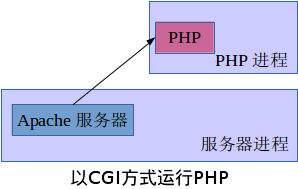
\includegraphics[scale=0.65]{php_cgi.png}
\end{figure}

为了弥补CGI的先天缺陷,以Apache模块方式运行PHP后,动态链接库php5apache2.dll或php4apache2.dll在Aapche服务启动的同时,将会被载入到与Apache服务相同的内存单元中,而且在PHP脚本解析期间不会增加额外的进程。

Apache模块可以在节省资源的同时提高系统运行效率,而且PHP的某些系统特性(例如数据库的持久连接等)只有在以Apache模块形式运行PHP时才会生效。



\begin{figure}[htbp]
\centering
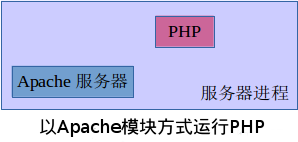
\includegraphics[scale=0.65]{php_apache_module.png}
\end{figure}

\subsection{Request Message}

客户端发起的请求信息(Request Message)包括请求行、(请求)头、空行和其他消息体。

\begin{compactitem}
\item 请求行,例如 GET /images/logo.gif HTTP/1.1 表示从/images 目录下请求 logo.gif文件。
\item (请求)头,例如 Accept-Language: en
\item 空行
\item 其他消息体
\end{compactitem}

请求行和标题必须以 <CR><LF> 作为结尾,空行内必须只有 <CR><LF> 而无其他空格。在 HTTP/1.1 协议中,所有的请求头(除 Host 外)都是可选的。例如,下面是一个HTTP 客户端与服务器之间会话的例子。



\begin{lstlisting}[language=bash]
GET / HTTP/1.1
Host:www.google.com
\end{lstlisting}

在客户端发起的请求的末尾有一个空行(以回车(CR)加换行(LF)的形式表示),其中请求信息的第一行指定方法、资源路径、协议版本,第二行是使用 HTTP/1.1 中必需的 header 来指定主机。

另外,在 HTTP 服务器返回的应答中的文件头之后也使用一个空行来隔开 header 和HTML 代码。




\begin{lstlisting}[language=bash]
HTTP/1.1 200 OK
Content-Length: 3059
Server: GWS/2.0
Date: Sat, 11 Jan 2003 02:44:04 GMT
Content-Type: text/html
Cache-control: private
Set-Cookie: PREF=ID=73d4aef52e57bae9:TM=1042253044:LM=1042253044:S=SMCc_HRPCQiqy
X9j; expires=Sun, 17-Jan-2038 19:14:07 GMT; path=/; domain=.google.com
Connection: keep-alive
<!-- HTML -->
\end{lstlisting}

HTTP/1.1 优化支持持续活跃连接,客户端可以连续多次发送请求、接收应答,而且批量多请求时,同一 TCP 连接在活跃(Keep-Live)间期内可以进行复用来避免重复 TCP初始握手活动,并减少网络负荷和响应周期。

此外,HTTP/1.1 支持应答到达前继续发送请求(通常是两个),称为“流线化”(stream)。

\subsection{Request Method}

HTTP/1.1 协议中共定义了八种方法(也叫“动作”)来以不同方式操作指定的资源。

OPTIONS 方法可使服务器传回该资源所支持的所有 HTTP 请求方法。用’*’ 来代替资源名称向 Web 服务器发送 OPTIONS 请求,则将返回响应的功能和方法,从而可以测试服务器功能是否正常运作。

HEAD 与 GET 方法一样,都是向服务器发出指定资源的请求。不过,服务器将不传回资源的正文部份,只是传回响应客户端请求的文件头,因此使用 HEAD 方法可以在不必传输全部内容的情况下,就可以获取其中“关于该资源的信息”(元信息或称元数据)。

GET 方法向指定的资源发出“显示”请求,因此 GET 方法应该只用在读取数据,而不应当被用于产生“副作用”的操作中。

另外,使用 GET 方法可以在请求 URL 中包含明文变量,一般情况下使用? 和 \&来隔开不同的变量。例如,在请求 URL(http://test.com/index.html?id=003\&title=test)中的变量和值分别为:

\begin{compactitem}
\item id=003
\item title=test
\end{compactitem}

POST 方法向指定资源提交数据并请求服务器进行处理(例如提交表单或者上传文件)。数据被包含在请求本文中,POST 请求可能会创建新的资源或修改现有资源,或二者皆有。

PUT 方法向指定资源位置上传其最新内容。

DELETE 方法请求服务器删除 Request-URI 所标识的资源。

TRACE 方法回显服务器收到的请求,主要用于测试或诊断。

CONNECT 方法由 HTTP/1.1 协议预留给能够将连接改为管道方式的代理服务器。通常用于 SSL 加密服务器的链接(经由非加密的 HTTP 代理服务器)。


请求方法的名称是区分大小写的,这样当某个请求所针对的资源不支持对应的请求方法的时候,服务器应当返回状态码 405(Method Not Allowed),当服务器不认识或者不支持对应的请求方法的时候,应当返回状态码 501(Not Implemented)。

HTTP 服务器至少应该实现 GET 和 HEAD 方法,其他方法都是可选的,而且特定的HTTP 服务器还能够扩展自定义的方法。例如,由 RFC5789 指定的 PATCH 方法用于将局部修改应用到资源。

HTTPS URI 方案和 HTTP 1.1 请求头都可以创建安全超文本协议连接,不过浏览器对后者的几乎没有任何支持,因此 HTTPS URI 方案仍是创建安全超文本协议连接的主要手段。

对于 GET 和 HEAD 方法而言,除了进行获取资源信息外,这些请求不应当再有其他意义。也就是说,这些方法应当被认为是“安全的”。客户端可能会使用其他“非安全”方法(例如 POST,PUT 及 DELETE)以特殊的方式(通常是按钮而不是超链接)来告知客户可能的后果(例如一个按钮控制的资金交易),或请求的操作可能是不安全的(例如某个文件将被上传或删除)。

在不考虑诸如错误或者过期等问题的情况下,若干次请求的副作用与单次请求相同或者根本没有副作用,那么这些请求方法就能够被视作“幂等”的,因此 GET,HEAD,PUT 和 DELETE 等方法都有这样的幂等属性。

假如某个由若干个请求做成的请求序列产生的结果在重复执行这个请求序列或者其中任何一个或多个请求后仍没有发生变化,则这个请求序列便是“幂等”的。但是,可能出现若干个请求做成的请求序列是“非幂等”的,即使这个请求序列中所有执行的请求方法都是幂等的。例如,这个请求序列的结果依赖于某个会在下次执行这个序列的过程中被修改的变量。

\subsection{Request Protocol}

Web 服务器支持的协议包括 HTTP、HTTPS、FTP、Telnet、news 和 gopher 等,并且协议可以指示浏览器使用特定的方法连接到 Web 服务器的特定端口。

使用不同的协议的情况下,浏览器获得的响应数据也是不同的。

通常情况下,Web 服务器根目录下包含特殊的文件(例如 index.html 等),因此 Web服务器在收到客户端请求时会主动以根目录下的文件来输出。

\subsection{UseCanonicalName}

UseCanonicalName字段可以指定Apache如何构造系统的URL、主机名和端口号。

\begin{compactitem}
\item Off说明使用ServerName的值;
\item On说明使用由客户端发送过来的服务器名和端口号。
\end{compactitem}




\subsection{Error Response}

如果网站根目录下找不到首页(index 文件),Web 服务器可能的错误显示方式包括:

\begin{compactitem}
\item 如果在 Options 中设置了 Indexes,那么相应目录下的所有文件都会被列出来,提供类似 FTP 的链接页面。
\item 如果没有指定 Index 则可能显示错误信息通知。
\end{compactitem}

例如,在 httpd.conf 中对错误回应有如下的设置:


\begin{lstlisting}[language=bash]
#
# Customizable error responses come in three flavors:
# 1) plain text 2) local redirects 3) external redirects
#
# Some examples:
#ErrorDocument 500 "The server made a boo boo."
#ErrorDocument 404 /missing.html
#ErrorDocument 404 "/cgi-bin/missing_handler.pl"
#ErrorDocument 402 http://www.example.com/subscription_info.html
#
\end{lstlisting}


在 Web 服务器的所有配置文件中只能有一个 ErrorDocument 设置,如果设置了多个相同的 ErrorDocument 值,则以较晚出现的设置为最终设置。

\begin{compactitem}
\item 100 ~ 199,基本信息
\item 200 ~ 299,客户端请求成功
\item 300 ~ 399,客户端请求需要其他额外的操作(例如重定向等)
\item 400 ~ 499,客户端请求无法完成(例如无法找到文件)
\item 500 ~ 599,Web服务器端错误
\end{compactitem}

\subsection{Access Permission}

Web 服务器的配置文件可以指定限制浏览来源的操作,还可以针对来源 IP 或网段进行限制\footnote{在实际生产环境中设置网段和 IP 的访问权限时,最好使用 iptables 来实现。}。


Apache httpd Server默认情况下的安全设置是拒绝一切访问,例如下面的指令禁止在任一目录下改变认证和访问控制。

\begin{lstlisting}[language=bash]
<Directory />
	Deny from all
	Allow Override None
</Directory>
\end{lstlisting}



默认的访问权限与allow和deny字段的处理顺序有关,而且allow和deny可以指定多个变量,其中:


\begin{compactitem}
\item allow字段用于设置可以访问服务器的客户端;
\item deny字段用于限制访问服务器的客户端。
\end{compactitem}


当deny和allow一起使用时,可以使用Order命令设置deny和allow的结合顺序。

\begin{compactitem}
\item \texttt{Order deny, allow}

以 deny 优先处理,没有写入规则的设置默认为 allow,常用于“拒绝所有,开放特定的条件”。

默认情况下允许所有客户端访问,且deny字段在allow字段之前被匹配。如果既匹配allow字段又匹配allow字段,则allow字段最终生效,也就是说allow覆盖deny。


\begin{lstlisting}[language=bash]
# 仅允许10.0.0.0/8网段的访问
Order deny, allow
Deny from all
Allow from 10.0.0.0/8
\end{lstlisting}

\item \texttt{Order allow, deny}

以 allow 优先处理,没有写入规则的设置默认为 deny,常用于“开放所有,拒绝特定的条件”。


默认情况下拒绝所有客户端访问,且allow字段在deny字段之前被匹配。如果既匹配allow字段又匹配deny字段,则deny字段最终生效,也就是说deny覆盖allow。


\begin{lstlisting}[language=bash]
# 限制www.test.com的访问
Order allow, deny
Allow from all
Deny from www.test.com
\end{lstlisting}

\item 如果 allow 和 deny 的规则中有重复的,则以默认的情况(Order 的规范)为主。
\end{compactitem}

下面的示例中拒绝 10.0.0.5,并对其他所有的主机开放访问,因此需要开放所有并拒绝特定的条件。



\begin{lstlisting}[language=bash]
# vim /etc/httpd/conf/httpd.conf
<Directory "/var/www/html">
	Options FollowSymLinks
	AllowOverride None
	Order allow,deny
	deny from 10.0.0.5
</Directory>
\end{lstlisting}

如果需要对内部受保护的目录(例如/var/www/html/db/进行设置仅有 192.168.1.0/200网段可以访问,可以进行如下的设置:




\begin{lstlisting}[language=bash]
# vim /etc/httpd/conf/httpd.conf
<Directory "/var/www/html/db">
	Options FollowSymLinks
	AllowOverride None
	Order deny, allow
	deny from all
	allow from 192.169.10/200
</Directory>
\end{lstlisting}

除了 Order 设置之外,还可以使用 Limit 来限制客户端能够进行操作的设置。例如,如果设置用户在指定的目录下仅能进行 GET、POST、OPTIONS 等操作,可以使用 Limit和 LimitExcept 如下的设置:


\begin{lstlisting}[language=bash]
# vim /etc/httpd/conf/httpd.conf
<Directory "/var/www/html">
	AllowOverride None
	Options FollowSymLinks
	<Limit GET POST OPTIONS>
		Order allow, deny
		Allow from all
	</Limit>
	<LimitExcept GET POST OPTIONS>
		Order deny, allow
		Deny from all
	</LimitExcept>
</Directory>
\end{lstlisting}

\subsection{User Management}

用户可以为httpd建立专用的用户和组来运行httpd子进程,否则以root用户运行httpd服务容易被攻击者通过漏洞利用或溢出攻击来获得系统的root权限,因此降低运行httpd用户的权限可以使攻击者无法以root身份远程联机或破坏。

在httpd.conf中可以通过User和Group字段分别设置对请求提供服务的httpd子进程运行时的用户和组。

\begin{lstlisting}[language=bash]
#
# If you wish httpd to run as a different user or group, you must run
# httpd as root initially and it will switch.  
#
# User/Group: The name (or #number) of the user/group to run httpd as.
# It is usually good practice to create a dedicated user and group for
# running httpd, as with most system services.
#
User apache
Group apache
# cat /etc/passwd | grep apache
apache:x:48:48:Apache:/usr/share/httpd:/sbin/nologin
\end{lstlisting}




\begin{lstlisting}[language=bash]

\end{lstlisting}




\begin{lstlisting}[language=bash]

\end{lstlisting}




\begin{lstlisting}[language=bash]

\end{lstlisting}




\begin{lstlisting}[language=bash]

\end{lstlisting}




\begin{lstlisting}[language=bash]

\end{lstlisting}




\begin{lstlisting}[language=bash]

\end{lstlisting}




\section{Server Logging}

为系统服务建立日志文件是必不可少的工作,否则网络中针对系统的开放端口的恶意连接尝试等攻击就无法记录,也就无法通过分析日志文件来监控运行状态,也无法分析出错误原因和找出安全隐患,因此在Apache httpd服务中至少要建立访问日志和错误日志文件来记录相关信息。

\begin{compactitem}
\item /var/log/httpd/access\_log 记录客户端正常的请求信息,可以用来分析热门网页等。
\item /var/log/httpd/error\_log 记录服务启动和运行过程中发生的错误、客户端请求错误以及主机设置错误等信息,可以用来检测404错误、文件权限设置错误和密码文件名输入错误等。
\end{compactitem}

\subsection{Error Log}


用户可以通过tail命令来动态检测httpd错误日志来排除故障。



\begin{lstlisting}[language=bash]
# tail -f /var/log/httpd/error_log
[Sun May 03 14:58:07.929011 2015] [mpm_prefork:notice] [pid 1783] AH00163: Apache/2.4.10 (Fedora) OpenSSL/1.0.1k-fips PHP/5.6.8 configured -- resuming normal operations
\end{lstlisting}

\begin{compactitem}
\item 错误发生的时间
\item 错误的级别(或严重性)
\item 错误的进程ID
\item 错误信息
\end{compactitem}


日志文件是纯文本信息而且增长很快,因此需要进行压缩和轮换,Apache 默认提供了/etc/logrotate.d/httpd 来处理日志。其中,开启 compress 可以进行日志压缩。




\begin{lstlisting}[language=bash]
# cat /etc/logrotate.d/httpd
/var/log/httpd/*log {
	missingok
	notifempty
	sharedscripts
	delaycompress
	postrotate
	/bin/systemctl reload httpd.service > /dev/null 2>/dev/null || true
	endscript
	# compress
}
\end{lstlisting}


\subsection{Access Log}


访问日志可以记录服务器处理的所有请求,这样可以检测访问服务器的客户端和被访问的文件。

访问日志的文件名和位置取决于CustomLog字段的设置,默认值如下:


\begin{lstlisting}[language=bash]
# cat /etc/httpd/conf/httpd.conf | grep CustomLog
<IfModule log_config_module>
    #
    # The following directives define some format nicknames for use with
    # a CustomLog directive (see below).
    #
    LogFormat "%h %l %u %t \"%r\" %>s %b \"%{Referer}i\" \"%{User-Agent}i\"" combined
    LogFormat "%h %l %u %t \"%r\" %>s %b" common

    <IfModule logio_module>
      # You need to enable mod_logio.c to use %I and %O
      LogFormat "%h %l %u %t \"%r\" %>s %b \"%{Referer}i\" \"%{User-Agent}i\" %I %O" combinedio
    </IfModule>

    #
    # The location and format of the access logfile (Common Logfile Format).
    # If you do not define any access logfiles within a <VirtualHost>
    # container, they will be logged here.  Contrariwise, if you *do*
    # define per-<VirtualHost> access logfiles, transactions will be
    # logged therein and *not* in this file.
    #
    #CustomLog "logs/access_log" common

    #
    # If you prefer a logfile with access, agent, and referer information
    # (Combined Logfile Format) you can use the following directive.
    #
    CustomLog "logs/access_log" combined
</IfModule>
\end{lstlisting}


combined和common都表示日志采用的格式,其中:

\begin{compactitem}
\item common表示通用日志格式,可以被日志分析识别;
\item combined表示组合类型日志,比通用日志格式增加了“引用页”和“浏览器识别”字段。
\end{compactitem}

访问日志的格式中使用类似printf()函数的格式字符串,使用LogFormat字段可以指定日志的格式和类型。

\begin{compactitem}
\item \%h表示发送请求到服务器的客户端IP地址。
\item \%l表示由客户端identd进程判断的RFC1413身份,不过除非在严格控制的内部网络中,否则\%l通常很不可靠,可以使用\texttt{-\%l}表示信息无效。

实际上,只有在将IndentityCheck指令设置为On时,httpd才会试图得到身份信息。

\item \%u表示HTTP认证系统得到的访问网页的客户标识(userid),例如环境变量REMOTE\_USER会被设置为userid并提供给CGI脚本。

\begin{compactitem}[$\circ$]
\item 如果状态码是401,表示客户未通过认证,那么userid无意义;
\item 如果网页没有设置密码保护,那么可以设置为\texttt{-\%u}。
\end{compactitem}

\item \%t表示服务器完成请求处理时的时间。

\item \texttt{\textbackslash "\%r\textbackslash"}表示客户端发出的包含相关信息的请求行,例如\texttt{GET / HTTP/1.1}。

\item \%>s表示服务器返回给客户端的状态码,可以用来指示请求的结果。

\begin{compactitem}[$\circ$]
\item 100 ~ 199,基本信息
\item 200 ~ 299,客户端请求成功
\item 300 ~ 399,客户端请求需要其他额外的操作(例如重定向等)
\item 400 ~ 499,客户端请求无法完成(例如无法找到文件)
\item 500 ~ 599,Web服务器端错误
\end{compactitem}

\item \%b表示返回给客户端的不包括响应头的字节数,\texttt{-\%b}表示没有信息返回,\texttt{\%B}表示希望记录为“0”的返回信息。

\item \texttt{\textbackslash "\{Referer\}i\textbackslash "}表示提交请求的网页。

\item \texttt{\textbackslash "\%\{User-Agent\}i\textbackslash "}表示客户端提供的浏览器识别信息。

\end{compactitem}

\section{Directory}





通常情况下,在访问某个网站时真正访问的仅仅是Web服务器中某个目录下的某个网页文件,不同的目录和文件组成了最终的网站。

在httpd.conf中基于目录块可以使用<Directory>对目录进行配置,而且<Directory>段中的命令的作用域是指定的目录及其所有子目录,不过使用.htaccess可以实现相同的效果。


\begin{lstlisting}[language=bash]
<Directory 目录>
控制语句
</Directory>
\end{lstlisting}

在设置网站整体的权限之外,可以使用由成对出现的<Directory></Directory>表示的Directory容器修改目录的权限。例如,下面的设置可以拒绝192.168.1.100的客户端访问某个目录内的文件。


\begin{lstlisting}[language=bash]
<Directory /doc>
	Order allow, deny
	Allow from all
	Deny from 192.168.1.100
</Directory>
\end{lstlisting}




\subsection{Root Directory}

下面是根目录默认设置:

\begin{lstlisting}[language=bash]
<Directory />
    AllowOverride none
    Require all denied
</Directory>
\end{lstlisting}

\begin{table}[htbp]
\centering
\caption{Options常用设置}
\begin{tabular}{|l|l|}
\hline
Options & 备注\\
\hline
FollowSymLinks & 允许在目录中使用符号链接\\
\hline
Indexes & 允许目录浏览,可以列出目录结构和子目录和文件\\
\hline
MultiViews & 允许内容协商的多重视图,例如提供多语言支持等\\
\hline
ExecCGI&允许执行CGI脚本\\
\hline
Includes & 允许服务器端包含(SSI)功能,和IIS/PWS的shtml功能相同\\
\hline
IncludesNoExec&允许服务器端包含(SSI)功能,但是不能执行CGI脚本\\
\hline
ALL&包含除MultiViews之外的所有特性。如果没有Options字段,默认为ALL\\
\hline
\end{tabular}
\end{table}

AllowOverride用于指定.htaccesss文件文件中的指令类型,从而限制.htaccess对相应类型命令的控制权。

\begin{compactitem}
\item None表示禁止使用.htaccess;
\item Options允许使用指定目录控制功能的命令;
\item Indexes允许使用目录索引类命令;
\item AuthConfig允许使用权限识别命令;
\item FileInfo允许使用文档控制类命令;
\item Limit允许使用主机访问控制类命令(Allow、Deny和Order)。
\end{compactitem}

默认情况下,Apache服务器允许使用.htaccess(即访问控制文件)对任意目录进行单独设置来覆盖主配置文件中的设置,而且修改.htaccess后可以即时生效,无需重启Apache服务器。

在启用CGI方式处理网络请求时,应该只允许特定的目录(例如cgi-bin)执行CGI功能,以防受到恶意攻击。

IncludesNoExec禁用“\#exec”和“\#exec CGI”,可以从ScriptAlias目录使用“\#include”虚拟CGI脚本。





\subsection{Document Directory}

下面是文档目录的默认设置:

\begin{lstlisting}[language=bash]
#
# Relax access to content within /var/www.
#
<Directory "/var/www">
    AllowOverride None
    # Allow open access:
    Require all granted
</Directory>

# Further relax access to the default document root:
<Directory "/var/www/html">
    #
    # Possible values for the Options directive are "None", "All",
    # or any combination of:
    #   Indexes Includes FollowSymLinks SymLinksifOwnerMatch ExecCGI MultiViews
    #
    # Note that "MultiViews" must be named *explicitly* --- "Options All"
    # doesn't give it to you.
    #
    # The Options directive is both complicated and important.  Please see
    # http://httpd.apache.org/docs/2.4/mod/core.html#options
    # for more information.
    #
    Options Indexes FollowSymLinks

    #
    # AllowOverride controls what directives may be placed in .htaccess files.
    # It can be "All", "None", or any combination of the keywords:
    #   Options FileInfo AuthConfig Limit
    #
    AllowOverride None

    #
    # Controls who can get stuff from this server.
    #
    Require all granted
</Directory>
\end{lstlisting}

\subsection{Directory Alias}

一般情况下,httpd 服务器默认的文档根目录为/var/www/html,如果需要发布到其他目录需要使用虚拟目录(alias)功能。


虚拟目录就是给一个实际目录起一个别名,这样就可以把不在文档目录中的目录纳入httpd服务管理。



\begin{lstlisting}[language=bash]
# phpMyAdmin - Web based MySQL browser written in php
# 
# Allows only localhost by default
#
# But allowing phpMyAdmin to anyone other than localhost should be considered
# dangerous unless properly secured by SSL

Alias /phpMyAdmin /usr/share/phpMyAdmin
Alias /phpmyadmin /usr/share/phpMyAdmin
\end{lstlisting}

\begin{compactitem}
\item 虚拟目录的名称和路径都不受实际目录名称和路径的限制,客户端不区分虚拟目录和实际目录。

\item 虚拟目录可以用于视频点播网站等需要大容量存储空间的硬盘扩容。

\item 虚拟目录不受目录移动和重命名等的限制,不会影响用户的访问。

\item 虚拟目录可以设置和实际目录相同的权限,并且攻击者无法猜测虚拟目录的实际路径。

\end{compactitem}

\begin{lstlisting}[language=bash]

\end{lstlisting}



\begin{lstlisting}[language=bash]

\end{lstlisting}



\begin{lstlisting}[language=bash]

\end{lstlisting}



\begin{lstlisting}[language=bash]

\end{lstlisting}



\begin{lstlisting}[language=bash]

\end{lstlisting}




\subsection{File Permission}

如果仅对某个文件设置权限,可以使用由成对出现的<Files></Files>表示的Files容器修改权限。


\begin{lstlisting}[language=bash]
<Files ~ "/var/www/html/robot.txt">
	Order allow, deny
	Allow from all
</Files>
\end{lstlisting}



\begin{lstlisting}[language=bash]

\end{lstlisting}

\section{Virtualhost}



虚拟主机(Virtual Host)让多个主机名称(host name)运行在在单一服务器(或是服务器组)上,从而实现多个域名和主机名绑定,而且可以单独支持每个单一的主机名称。

通过将服务器的某项或者全部服务内容逻辑划分为多个服务单位,对外可以表现为多个服务器,从而充分利用服务器硬件资源。如果划分是系统级别的,则称为虚拟服务器。例如,如果使用 dig 等检查 IP,可能发现不同的网址可能指向同一个 IP。

单一主机(或服务器组)支撑的所有的虚拟主机中,彼此之间可以共用相同的配置设置。另外,相同主机内的虚拟主机可以共用彼此的程序集(Process Pool),从而可以缩短对客户端的响应时间。

虚 拟 主 机 的 实 现 方 式 主 要 有 三 种: 网 址 名 称 对 应 (Name-based)、IP 地 址 对 应(IP-based)以及 Port 端口号对应(Port-based)。

\begin{compactitem}
\item 网址名称对应(Name-based)

网址名称对应(Name-based)通过辨识客户端所提供的网址来决定其所对应的服务,可以有效的减少 IP 地址的占用,缺点是必须仰赖 DNS 名称对应服务的支持。

若 DNS 服务中断,则对应此名称的服务也会无法取用。

\item IP 地址对应(IP-based)

IP 地址对应(IP-based)是指在同一部服务器上,借由同一份配置设置、不同的 IP来管理多个服务。

\item Port 端口号对应(Port-based)

近似于 IP 地址对应,不过是在同一个 IP 之下利用不同的 Port 端口号来区别不同的服务,藉以快速创建多个虚拟主机。例如:

\begin{lstlisting}[language=bash]
192.168.0.1:80
192.168.0.1:8080
192.168.0.1:8888
\end{lstlisting}

\end{compactitem}



如果每个网站拥有不同的 IP 地址,则虚拟主机可以是” 基于 IP” 的;如果只有一个IP 地址,也可以是” 基于主机名” 的,其实对最终用户是透明的。例如,Apache 是率先支持基于 IP 的虚拟主机的服务器之一,1.1 及其更新版本同时支持基于 IP 和基于主机名的虚拟主机。

如果要调试虚拟主机配置,可以使用 httpd 的-S 命令行开关来输出虚拟主机的配置。






\begin{lstlisting}[language=bash]
// a synonym for -t -D DUMP_VHOSTS -D DUMP_RUN_CFG
# /usr/sbin/httpd -S
VirtualHost configuration:
ServerRoot: "/etc/httpd"
Main DocumentRoot: "/var/www/html"
Main ErrorLog: "/etc/httpd/logs/error_log"
Mutex authdigest-client: using_defaults
Mutex lua-ivm-shm: using_defaults
Mutex proxy: using_defaults
Mutex authn-socache: using_defaults
Mutex default: dir="/run/httpd/" mechanism=default
Mutex mpm-accept: using_defaults
Mutex authdigest-opaque: using_defaults
Mutex proxy-balancer-shm: using_defaults
Mutex rewrite-map: using_defaults
PidFile: "/run/httpd/httpd.pid"
Define: DUMP_VHOSTS
Define: DUMP_RUN_CFG
User: name="apache" id=48
Group: name="apache" id=48
\end{lstlisting}


一般情况下,虚拟主机的配置文件 vhosts.conf 保存为/etc/httpd/conf.d/vhosts.conf,而且虚拟主机的设置中至少要有 ServerName 和 DocumentRoot。

如果没有针对 SELinux 设置 httpd 可以读取的文件系统,则虚拟主机无法提供浏览功能。


\subsection{IP}


下面的示例说明使用httpd实现基于IP的虚拟主机,这样需要为Web服务器的网卡绑定多个IP地址。


\begin{lstlisting}[language=bash]
# ifconfig eth0:0 192.168.1.11 netmask 255.255.255.0
# ifconfig eth0:1 192.168.1.12 netmask 255.255.255.0

# cat > /etc/httpd/conf/httpd.conf
...

<VirtualHost 192.168.1.10:80>
	DocumentRoot /var/www/html/www.example.com
	ServerName www.example.com
</VirtualHost>

<VirtualHost 192.168.1.11:80>
	DocumentRoot /var/www/html/bbs.example.com
	ServerName bbs.example.com
</VirtualHost>

<VirtualHost 192.168.1.12:80>
	DocumentRoot /var/www/html/test.example.com
	ServerName test.example.com
</VirtualHost>

# mkdir -p /var/www/html/www.example.com
# mkdir -p /var/www/html/bbs.example.com
# mkdir -p /var/www/html/test.example.com

# echo "Welcome to www.example.com" > /var/www/html/www.example.com/index.html
# echo "Welcome to bbs.example.com" > /var/www/html/bbs.example.com/index.html
# echo "Welcome to test.example.com" > /var/www/html/test.example.com/index.html

# chmod -R 755 /var/www/html/bbs.example.com
# chmod -R 755 /var/www/html/test.example.com
\end{lstlisting}




\begin{lstlisting}[language=bash]

\end{lstlisting}





\begin{lstlisting}[language=bash]

\end{lstlisting}





\begin{lstlisting}[language=bash]

\end{lstlisting}





\begin{lstlisting}[language=bash]

\end{lstlisting}



\subsection{Domain}


随着基于IP地址的虚拟主机的增加,采用IP地址的方式会导致IP地址的极大浪费,因此通常情况下都是基于域名来实现虚拟主机。


在主配置文件中添加NameVirtualHost字段,这样就可以为多个虚拟主机统一配置端口,从而就可以开启基于域名的虚拟主机功能。例如,在下面的示例中可以为虚拟主机建立相应的站点目录,设置网页文件,并且所有的域名(这里是www.example.com、bbs.example.com、test.example.com)都可以指向服务器的IP地址,从而完成虚拟主机的配置。


\begin{lstlisting}[language=bash]
# cat > /etc/httpd/conf/httpd.conf
...
NameVirtualHost *:80
<VirtualHost *:80>
	ServerName www.example.com
	DocumentRoot /var/www/html/www.example.com/
</VirtualHost>

<VirtualHost *:80>
	ServerName bbs.example.com
	DocumentRoot /var/www/html/bbs.example.com/
</VirtualHost>

<VirtualHost *:80>
	ServerName test.example.com
	DocumentRoot /var/www/html/test.example.com/
</VirtualHost>
\end{lstlisting}




\begin{lstlisting}[language=bash]

\end{lstlisting}




\begin{lstlisting}[language=bash]

\end{lstlisting}


\section{Module}

\subsection{Extension}

httpd 的主要配置文件位于/etc/httpd/conf/httpd.conf,其他的配置文件则位于/etc/httpd/conf.d/*.conf。


\begin{lstlisting}[language=bash]
$ ll /etc/httpd/conf.d/
-rw-r--r--. 1 root root 2893 Jul 23 18:29 autoindex.conf
-rw-r--r--. 1 root root 295 Jul 23 18:24 manual.conf
-rw-r--r--. 1 root root 747 Nov 21 20:09 php.conf
-rw-r--r--. 1 root root 366 Jul 23 18:31 README
-rw-r--r--. 1 root root 298 Sep 12 18:59 squid.conf
-rw-r--r--. 1 root root 1252 Jul 23 18:24 userdir.conf
-rw-r--r--. 1 root root 516 Jul 23 18:24 welcome.conf
\end{lstlisting}


httpd 本身只支持静态网页文件,如果需要处理动态网页则需要配合相应的模块,这些模块一般位于/usr/lib/httpd/modules(或/usr/lib64/httpd/modules)。


\begin{lstlisting}[language=bash]
$ ll /usr/lib64/httpd/modules
-rwxr-xr-x. 1 root root 4347080 Nov 21 20:10 libphp5.so
-rwxr-xr-x. 1 root root 4561080 Nov 21 20:10 libphp5-zts.so
-rwxr-xr-x. 1 root root 11208 Jul 23 18:31 mod_access_compat.so
-rwxr-xr-x. 1 root root 11168 Jul 23 18:31 mod_actions.so
-rwxr-xr-x. 1 root root 15368 Jul 23 18:31 mod_alias.so
-rwxr-xr-x. 1 root root 11144 Jul 23 18:31 mod_allowmethods.so
-rwxr-xr-x. 1 root root 11088 Jul 23 18:31 mod_asis.so
-rwxr-xr-x. 1 root root 15360 Jul 23 18:31 mod_auth_basic.so
-rwxr-xr-x. 1 root root 36056 Jul 23 18:31 mod_auth_digest.so
-rwxr-xr-x. 1 root root 11152 Jul 23 18:31 mod_authn_anon.so
-rwxr-xr-x. 1 root root 15368 Jul 23 18:31 mod_authn_core.so
-rwxr-xr-x. 1 root root 15272 Jul 23 18:31 mod_authn_dbd.so
-rwxr-xr-x. 1 root root 11192 Jul 23 18:31 mod_authn_dbm.so
-rwxr-xr-x. 1 root root 11168 Jul 23 18:31 mod_authn_file.so
-rwxr-xr-x. 1 root root 19544 Jul 23 18:31 mod_authn_socache.so
-rwxr-xr-x. 1 root root 23728 Jul 23 18:31 mod_authz_core.so
-rwxr-xr-x. 1 root root 15320 Jul 23 18:31 mod_authz_dbd.so
-rwxr-xr-x. 1 root root 15304 Jul 23 18:31 mod_authz_dbm.so
-rwxr-xr-x. 1 root root 15296 Jul 23 18:31 mod_authz_groupfile.so
-rwxr-xr-x. 1 root root 11200 Jul 23 18:31 mod_authz_host.so
-rwxr-xr-x. 1 root root 11136 Jul 23 18:31 mod_authz_owner.so
-rwxr-xr-x. 1 root root 11160 Jul 23 18:31 mod_authz_user.so
-rwxr-xr-x. 1 root root 40072 Jul 23 18:31 mod_autoindex.so
-rwxr-xr-x. 1 root root 11152 Jul 23 18:31 mod_buffer.so
-rwxr-xr-x. 1 root root 36096 Jul 23 18:31 mod_cache_disk.so
-rwxr-xr-x. 1 root root 77320 Jul 23 18:31 mod_cache.so
-rwxr-xr-x. 1 root root 36064 Jul 23 18:31 mod_cache_socache.so
-rwxr-xr-x. 1 root root 36088 Jul 23 18:31 mod_cgid.so
-rwxr-xr-x. 1 root root 27712 Jul 23 18:31 mod_cgi.so
-rwxr-xr-x. 1 root root 23600 Jul 23 18:31 mod_charset_lite.so
-rwxr-xr-x. 1 root root 11096 Jul 23 18:31 mod_data.so
-rwxr-xr-x. 1 root root 56984 Jul 23 18:31 mod_dav_fs.so
-rwxr-xr-x. 1 root root 19632 Jul 23 18:31 mod_dav_lock.so
-rwxr-xr-x. 1 root root 101992 Jul 23 18:31 mod_dav.so
-rwxr-xr-x. 1 root root 23568 Jul 23 18:31 mod_dbd.so
-rwxr-xr-x. 1 root root 35944 Jul 23 18:31 mod_deflate.so
-rwxr-xr-x. 1 root root 11176 Jul 23 18:31 mod_dialup.so
-rwxr-xr-x. 1 root root 15288 Jul 23 18:31 mod_dir.so
-rwxr-xr-x. 1 root root 11192 Jul 23 18:31 mod_dumpio.so
-rwxr-xr-x. 1 root root 11160 Jul 23 18:31 mod_echo.so
-rwxr-xr-x. 1 root root 11176 Jul 23 18:31 mod_env.so
-rwxr-xr-x. 1 root root 15320 Jul 23 18:31 mod_expires.so
-rwxr-xr-x. 1 root root 23552 Jul 23 18:31 mod_ext_filter.so
-rwxr-xr-x. 1 root root 15408 Jul 23 18:31 mod_file_cache.so
-rwxr-xr-x. 1 root root 19424 Jul 23 18:31 mod_filter.so
-rwxr-xr-x. 1 root root 23752 Jul 23 18:31 mod_headers.so
-rwxr-xr-x. 1 root root 11192 Jul 23 18:31 mod_heartbeat.so
-rwxr-xr-x. 1 root root 23592 Jul 23 18:31 mod_heartmonitor.so
-rwxr-xr-x. 1 root root 52520 Jul 23 18:31 mod_include.so
-rwxr-xr-x. 1 root root 28120 Jul 23 18:31 mod_info.so
-rwxr-xr-x. 1 root root 11136 Jul 23 18:31 mod_lbmethod_bybusyness.so
-rwxr-xr-x. 1 root root 11136 Jul 23 18:31 mod_lbmethod_byrequests.so
-rwxr-xr-x. 1 root root 11128 Jul 23 18:31 mod_lbmethod_bytraffic.so
-rwxr-xr-x. 1 root root 15320 Jul 23 18:31 mod_lbmethod_heartbeat.so
-rwxr-xr-x. 1 root root 28192 Jul 23 18:31 mod_log_config.so
-rwxr-xr-x. 1 root root 15392 Jul 23 18:31 mod_log_debug.so
-rwxr-xr-x. 1 root root 11216 Jul 23 18:31 mod_log_forensic.so
-rwxr-xr-x. 1 root root 11232 Jul 23 18:31 mod_logio.so
-rwxr-xr-x. 1 root root 133424 Jul 23 18:31 mod_lua.so
-rwxr-xr-x. 1 root root 19440 Jul 23 18:31 mod_macro.so
-rwxr-xr-x. 1 root root 27736 Jul 23 18:31 mod_mime_magic.so
-rwxr-xr-x. 1 root root 23616 Jul 23 18:31 mod_mime.so
-rwxr-xr-x. 1 root root 60960 Jul 23 18:31 mod_mpm_event.so
-rwxr-xr-x. 1 root root 31880 Jul 23 18:31 mod_mpm_prefork.so
-rwxr-xr-x. 1 root root 48432 Jul 23 18:31 mod_mpm_worker.so
-rwxr-xr-x. 1 root root 36000 Jul 23 18:31 mod_negotiation.so
-rwxr-xr-x. 1 root root 52136 Jul 23 18:31 mod_proxy_ajp.so
-rwxr-xr-x. 1 root root 48176 Jul 23 18:31 mod_proxy_balancer.so
-rwxr-xr-x. 1 root root 19400 Jul 23 18:31 mod_proxy_connect.so
-rwxr-xr-x. 1 root root 15280 Jul 23 18:31 mod_proxy_express.so
-rwxr-xr-x. 1 root root 19376 Jul 23 18:31 mod_proxy_fcgi.so
-rwxr-xr-x. 1 root root 11152 Jul 23 18:31 mod_proxy_fdpass.so
-rwxr-xr-x. 1 root root 44184 Jul 23 18:31 mod_proxy_ftp.so
-rwxr-xr-x. 1 root root 39944 Jul 23 18:31 mod_proxy_http.so
-rwxr-xr-x. 1 root root 19464 Jul 23 18:31 mod_proxy_scgi.so
-rwxr-xr-x. 1 root root 118608 Jul 23 18:31 mod_proxy.so
-rwxr-xr-x. 1 root root 19352 Jul 23 18:31 mod_proxy_wstunnel.so
-rwxr-xr-x. 1 root root 11128 Jul 23 18:31 mod_ratelimit.so
-rwxr-xr-x. 1 root root 11160 Jul 23 18:31 mod_reflector.so
-rwxr-xr-x. 1 root root 15304 Jul 23 18:31 mod_remoteip.so
-rwxr-xr-x. 1 root root 15320 Jul 23 18:31 mod_reqtimeout.so
-rwxr-xr-x. 1 root root 15344 Jul 23 18:31 mod_request.so
-rwxr-xr-x. 1 root root 69032 Jul 23 18:31 mod_rewrite.so
-rwxr-xr-x. 1 root root 40312 Jul 23 18:31 mod_sed.so
-rwxr-xr-x. 1 root root 15328 Jul 23 18:31 mod_setenvif.so
-rwxr-xr-x. 1 root root 11240 Jul 23 18:31 mod_slotmem_plain.so
-rwxr-xr-x. 1 root root 19488 Jul 23 18:31 mod_slotmem_shm.so
-rwxr-xr-x. 1 root root 15328 Jul 23 18:31 mod_socache_dbm.so
-rwxr-xr-x. 1 root root 11192 Jul 23 18:31 mod_socache_memcache.so
-rwxr-xr-x. 1 root root 23568 Jul 23 18:31 mod_socache_shmcb.so
-rwxr-xr-x. 1 root root 15272 Jul 23 18:31 mod_speling.so
-rwxr-xr-x. 1 root root 23448 Jul 23 18:31 mod_status.so
-rwxr-xr-x. 1 root root 15272 Jul 23 18:31 mod_substitute.so
-rwxr-xr-x. 1 root root 11168 Jul 23 18:31 mod_suexec.so
-rwxr-xr-x. 1 root root 11112 Jul 23 18:31 mod_systemd.so
-rwxr-xr-x. 1 root root 11144 Jul 23 18:31 mod_unique_id.so
-rwxr-xr-x. 1 root root 15312 Jul 23 18:31 mod_unixd.so
-rwxr-xr-x. 1 root root 11168 Jul 23 18:31 mod_userdir.so
-rwxr-xr-x. 1 root root 15320 Jul 23 18:31 mod_usertrack.so
-rwxr-xr-x. 1 root root 11104 Jul 23 18:31 mod_version.so
-rwxr-xr-x. 1 root root 15280 Jul 23 18:31 mod_vhost_alias.so
-rwxr-xr-x. 1 root root 19480 Jul 23 18:31 mod_watchdog.so
\end{lstlisting}

用户可通过简单的 API 扩充,将 Perl/Python/PHP 等解释器编译到 HTTP 服务器中。例如,httpd 使用的 PHP 模块就是/usr/lib64/httpd/modules/libphp5.so,相应的 PHP 设置文件则位于/etc/httpd/conf.d/php.conf,并且在其中设置了由 PHP 产生的 session和 soap 的存储目录等信息。


\begin{lstlisting}[language=bash]
$ vim /etc/httpd/conf.d/php.conf
#
# Cause the PHP interpreter to handle files with a .php extension.
#
<FilesMatch \.php$>
	SetHandler application/x-httpd-php
</FilesMatch>
#
# Allow php to handle Multiviews
#
AddType text/html .php
#
# Add index.php to the list of files that will be served as directory indexes.
#
DirectoryIndex index.php
#
# Uncomment the following lines to allow PHP to pretty-print .phps files as PHP source code:
#
#<FilesMatch \.phps$>
#
SetHandler application/x-httpd-php-source
#</FilesMatch>
#
# Apache specific PHP configuration options those can be override in each configured vhost
#
php_value session.save_handler "files"
php_value session.save_path "/var/lib/php/session"
php_value soap.wsdl_cache_dir "/var/lib/php/wsdlcache"
\end{lstlisting}

不过,PHP 本身的主要配置文件为/etc/php.ini,其中包含了 PHP 的全部设置选项。

对于 PHP 的额外扩展配置则保存在/etc/php.d 和/etc/php-zts.d 中。


\begin{lstlisting}[language=bash]
$ ll /etc/php.d
-rw-r--r--. 1 root root 47 Nov 21 20:09 bz2.ini
-rw-r--r--. 1 root root 57 Nov 21 20:09 calendar.ini
-rw-r--r--. 1 root root 51 Nov 21 20:09 ctype.ini
-rw-r--r--. 1 root root 49 Nov 21 20:09 curl.ini
-rw-r--r--. 1 root root 47 Nov 21 20:09 dom.ini
-rw-r--r--. 1 root root 49 Nov 21 20:09 exif.ini
-rw-r--r--. 1 root root 57 Nov 21 20:09 fileinfo.ini
-rw-r--r--. 1 root root 47 Nov 21 20:09 ftp.ini
-rw-r--r--. 1 root root 55 Nov 21 20:09 gettext.ini
-rw-r--r--. 1 root root 51 Nov 21 20:09 iconv.ini
-rw-r--r--. 1 root root 51 Aug 1 14:50 json.ini
-rw-r--r--. 1 root root 55 Nov 21 20:09 mysqlnd.ini
-rw-r--r--. 1 root root 69 Nov 21 20:09 mysqlnd_mysqli.ini
-rw-r--r--. 1 root root 67 Nov 21 20:09 mysqlnd_mysql.ini
-rw-r--r--. 1 root root 47 Nov 21 20:09 pdo.ini
-rw-r--r--. 1 root root 63 Nov 21 20:09 pdo_mysqlnd.ini
-rw-r--r--. 1 root root 61 Nov 21 20:09 pdo_sqlite.ini
-rw-r--r--. 1 root root 49 Nov 21 20:09 phar.ini
-rw-r--r--. 1 root root 51 Nov 21 20:09 posix.ini
-rw-r--r--. 1 root root 51 Nov 21 20:09 shmop.ini
-rw-r--r--. 1 root root 59 Nov 21 20:09 simplexml.ini
-rw-r--r--. 1 root root 55 Nov 21 20:09 sockets.ini
-rw-r--r--. 1 root root 55 Nov 21 20:09 sqlite3.ini
-rw-r--r--. 1 root root 55 Nov 21 20:09 sysvmsg.ini
-rw-r--r--. 1 root root 55 Nov 21 20:09 sysvsem.ini
-rw-r--r--. 1 root root 55 Nov 21 20:09 sysvshm.ini
-rw-r--r--. 1 root root 59 Nov 21 20:09 tokenizer.ini
-rw-r--r--. 1 root root 101 Nov 17 20:47 xdebug.ini
-rw-r--r--. 1 root root 47 Nov 21 20:09 xml.ini
-rw-r--r--. 1 root root 59 Nov 21 20:09 xmlreader.ini
-rw-r--r--. 1 root root 49 Nov 21 20:09 xml_wddx.ini
-rw-r--r--. 1 root root 59 Nov 21 20:09 xmlwriter.ini
-rw-r--r--. 1 root root 47 Nov 21 20:09 xsl.ini
\end{lstlisting}

一般情况下,httpd 服务器默认的文档根目录为/var/www/html,其中的设置包括:

\begin{compactitem}
\item 错误信息位于/var/www/error
\item CGI 位于/var/www/cgi-bin
\item 图标位于/var/www/icons
\item 日志文件位于/var/log/httpd
\end{compactitem}

httpd 的可执行文件为/usr/sbin/httpd,而且其主要的环境检测和执行文件是/usr/sbin/apachectl,用于在启动 httpd 服务器时检测系统设置。

httpd 本身提供了基本的密码保护方式,这样就可以在用户登录某些网页时进行帐号/密码验证,其中密码使用/usr/bin/htpasswd 来产生。

如果使用 MySQL 数据库,则其配置文件位于/etc/my.conf,默认情况下数据库位于/var/lib/mysql。其中,与 PHP 配合使用的 MySQL 接口文件位于/usr/lib64/mysql。

为了产生由 MySQL 数据库驱动的 PHP 应用程序,需要在相应的配置中中对 PHP 支持的 MySQL 接口等进行设置。

\begin{compactitem}
\item /etc/php.d/mysqlnd.ini
\item /etc/php.d/mysqlnd\_mysqli.ini
\item /etc/php.d/mysqlnd\_mysql.ini
\item /etc/php.d/pdo\_mysqlnd.ini
\end{compactitem}

PHP 是动态语言,其程序中的值需要在运行时才能确定,因此如果需要安装 PHP 加速器等组件时需要/usr/bin/phpize 来辅助 PHP 扩展的编译。

一般情况下,编译安装 PHP 扩展时需要的头文件等都位于/usr/include/php 中。


\subsection{mod\_pagespeed}


PageSpeed (mod\_pagespeed) 是 Google开放的网页加速模块,支持Apache和Nginx服务器。 

64位系统:

\begin{lstlisting}[language=bash]
# wget https://dl-ssl.google.com/dl/linux/direct/mod-pagespeed-stable_current_x86_64.rpm
# rpm -ivh mod-pagespeed-stable_current_x86_64.rpm
\end{lstlisting}

32位系统:


\begin{lstlisting}[language=bash]
# wget https://dl-ssl.google.com/dl/linux/direct/mod-pagespeed-stable_current_i386.rpm
# rpm -ivh mod-pagespeed-stable_current_i386.rpm
\end{lstlisting}


如果把Pagespeed模块的仓库文件存到/etc/yum.repos.d/,这样就可以使用YUM来安装mode\_pagespeed。

\begin{lstlisting}[language=bash]
$ sudo yum install mod-pagespeed
\end{lstlisting}

用户可以通过/etc/httpd/conf.d/目录下的pagespeed.conf和pagespeed\_libraries.conf文件来设置mod\_pagespeed,并且通过重启Apache服务器来使配置生效。


\subsection{mod\_security}

mod\_security是Apache的安全模块,可以预防多种针对网页的攻击,例如远程代码执行、SQL注入和路径扫描等。




\begin{lstlisting}[language=bash]

\end{lstlisting}

用户可以直接下载并安装mod\_security模块:

CentOS/RHEL:


\begin{lstlisting}[language=bash]
$ sudo yum install mod_security
$ sudo systemctl restart httpd
\end{lstlisting}



Debian/Ubuntu

\begin{lstlisting}[language=bash]
$ sudo apt-get install libapache-mod-security
$ sudo a2enmod mod-security
$ sudo /etc/init.d/apache2 force-reload
\end{lstlisting}


也可以下载mod\_security的源代码并进行编译安装。


\begin{lstlisting}[language=bash]
$ sudo yum install gcc make httpd-devel libxml2 pcre-devel libxml2-devel curl-devel git
$ wget https://www.modsecurity.org/tarball/2.9.0/modsecurity-2.9.0.tar.gz
$ tar xzf modsecurity-apache_2.9.0.tar.gz
$ cd modsecurity-apache_2.9.0
$ ./configure
$ make && sudo make install
$ sudo cp modsecurity.conf-recommended /etc/httpd/conf.d/modsecurity.conf
$ sudo cp unicode.mapping /etc/httpd/conf.d/
\end{lstlisting}


在/etc/httpd/httpd.conf中加入mod\_security模块的配置信息来通过重启Apache载入mod\_security。


\begin{lstlisting}[language=bash]
LoadModule security2_module modules/mod_security2.so
<IfModule security2_module>
    Include conf.d/modsecurity.conf
</IfModule>
 
Include modsecurity-crs/modsecurity_crs_10_config.conf
Include modsecurity-crs/base_rules/*.conf
\end{lstlisting}






\begin{lstlisting}[language=bash]

\end{lstlisting}




\begin{lstlisting}[language=bash]

\end{lstlisting}





\begin{lstlisting}[language=bash]

\end{lstlisting}




\begin{lstlisting}[language=bash]

\end{lstlisting}





\section{Security}



使用 HTTP 协议来传输数据时都是以明文传送的,HTTPS 协议使用 SSL 加密机制来传输数据。



如果客户端和服务器同时支持 SSL(Secure Socket Layer)协议,那么服务器将产生公钥并向 CA(Certificate Authorities)注册,客户端浏览器可以主动向 CA 确认服务器端的公钥是否是合法的,如果合法则建立与服务器的连接,否则将发出警告信息来告知用户。

\subsection{Encryption}

为了保证机密信息被安全传输,并且有效识别双方的身份,数据加密和数字签名技术被引入到Web客户端和服务器中来对数据进行加密和签名。

\begin{compactitem}
\item 数据加密技术可以防止合法接收者之外的人获取信息系统中的机密信息。

\item 数字签名技术可以使用数字证书来对信息进行签名以实现信息的不可否认性。
\end{compactitem}

用户使用数学方法对原始信息进行加密来实现数据的再组织,使得重组后在网络上公开传输的内容变成对于非法接收者来说无效的信息,只有掌握正确的密钥的合法的接收者才能通过解密来得到原始数据。

\begin{compactitem}
\item 对称加密技术(例如DES)的发送方使用的加密密钥和接收方使用的解密密钥是相同的。

\item 非对称加密技术(例如RSA)要求密钥成对出现并彼此关联,其中用于加密的公钥可以对外界公开,但是用于解密的私钥必须由接收者自己保管。
\end{compactitem}

\subsection{Signature}

在信息传输过程中,单纯采用加密来保证数据的保密性还是存在缺陷的,无法证明信息的发送方身份。

为了使信息(例如合同和钱款往来)无法否认,可以使用数字签名(Digital Signature)技术来保证信息是由签名者自己签名发送的,而且接收方可以验证信息自签发后是否进行过任何修改。

数字签名的过程就是发送者根据待发送的信息和用自身私钥加密的数字摘要组合成数字签名,私钥仅为发送者本人所有,因此可以产生别人无法生成的文件,也就实现了数字签名。



\begin{compactitem}
\item 签名者不能否认或难以否认数字签名;
\item 接收方可以通过检查真实签发的数字证书文件来验证数据完整性。
\end{compactitem}

数字证书(Digital Certificate)是一个经证书授权中心数字签名的包含公开密钥拥有着信息以及公开密钥的文件,最简单的证书包含一个公开密钥、名称以及证书授权中心的数字签名,因此数字证书是标志网络用户身份信息的一系列数据,可以用来在网络通信中识别通信各方的身份。例如,现实中的每一个公司都要拥有工商执照来表明各自的身份或某种资格。

以数字证书为核心的加密技术可以对网络上传输的信息进行加密和解密、数字签名和签名验证,确保网上传递信息的机密性、完整性,交易实体身份的真实性,以及签名信息的不可否认性,从而保障网络应用的安全性。

数字证书签发机构(Certification Authority)管理数字证书的申请者发放、管理和取消,因此和现实中的工商业管理机构——工商行政管理局的职能类似,它们都可以检查证书持有者身份的合法性,并签发证书(用数学方法在证书上签名)来防止证书被伪造或篡改。

SSL(Secure Sockets Layer)是一种国际标准的加密和身份认证通信协议,可以用于Web浏览器和服务器之间的身份认证和加密数据传输,这样SSL通过数字证书和加密技术来实现在Web浏览器和服务器之间的通信无法被窃听,从而为通信双方建立起安全的、可信任的信息通道。

SSL最初由Netscape开发并内置于浏览器中来对数据进行压缩和加密操作,并返回通过网络传送回的数据,HTTPS(HTTP Secure)开始时就是使用SSL作为HTTP应用层的子层。

TLS(Transport Layer Security)及其前身 SSL(Secure Sockets Layer)是一种为互联网通信提供安全及数据完整性保障安全协议。

openssl命令可以为CA创建一个RSA私有密钥,也可以查看密钥的内容。



\begin{lstlisting}[language=bash]
# openssl genrsa -des3 -out ca.key 1024
Generating RSA private key, 1024 bit long modulus
.............++++++
..............................++++++
e is 65537 (0x10001)
Enter pass phrase for ca.key:
Verifying - Enter pass phrase for ca.key:
# chmod 400 ca.key
# ls -l ca.key
-r--------. 1 root root 963 May  4 23:15 ca.key
# openssl rsa -noout -text -in ca.key 
Enter pass phrase for ca.key:
Private-Key: (1024 bit)
modulus:
    00:c2:0b:93:4a:83:61:8b:e9:c8:e5:4a:9a:aa:c4:
    22:92:ac:de:84:6d:39:12:93:94:c5:02:b1:a1:2a:
    89:e6:07:41:6c:e8:66:fe:9c:11:81:9f:1f:ef:06:
    c5:3a:e8:28:dc:ba:0b:a6:45:92:cd:4e:5b:81:d9:
    e8:21:9c:9c:e4:01:5a:b3:44:0a:1b:9a:aa:62:a8:
    64:e3:24:47:43:33:bc:a6:8f:50:ad:b0:01:4b:71:
    8e:16:3a:f7:91:49:17:eb:ac:35:17:34:ed:35:19:
    6e:1e:f7:0a:f0:87:a0:e9:a5:3f:bc:12:8f:b1:a8:
    5e:5a:36:5e:df:20:88:ad:4d
publicExponent: 65537 (0x10001)
privateExponent:
    63:40:ec:7c:26:ab:94:97:66:6c:f2:36:1e:b6:e8:
    40:42:30:27:68:7e:d2:e3:ae:2a:ff:6f:c0:52:33:
    ea:f7:37:1d:ef:da:0e:cd:e1:9e:7d:b8:25:d9:3e:
    b5:1c:df:19:d8:07:f1:6a:90:e6:76:f8:13:79:54:
    65:2c:e8:8a:4a:0b:3e:d1:48:77:78:e5:a0:54:6f:
    c1:bb:e5:33:27:95:13:5e:ff:8e:23:ad:da:c1:4b:
    1b:78:63:80:0c:48:04:8a:47:c0:7e:b3:71:53:63:
    b9:0a:c1:08:3f:61:04:0d:5f:1f:34:43:ad:ff:f2:
    77:44:34:d1:19:89:8f:b9
prime1:
    00:fb:2e:9f:be:a1:30:2f:5a:ce:4d:a9:4d:db:eb:
    a3:d3:30:8a:08:f0:88:f5:00:28:10:c6:37:43:f2:
    c1:28:c0:a0:37:4a:f3:aa:95:b2:cf:95:13:c8:3f:
    84:2e:ea:89:45:b0:6f:73:f0:fe:8d:79:b4:da:a5:
    ee:8d:7d:83:eb
prime2:
    00:c5:c4:64:8e:fd:e8:47:16:c0:a5:b1:d6:59:c3:
    3a:f6:7c:6b:0f:99:f1:f7:90:6a:83:73:e8:0a:8f:
    c0:cf:02:42:b7:cb:95:f7:65:3d:5a:42:46:70:c6:
    9a:ba:aa:d5:80:d1:0c:2b:7f:14:d3:fd:61:3b:ad:
    89:23:a2:1d:a7
exponent1:
    00:f2:32:c5:d3:d1:a7:1d:b2:48:85:38:00:1c:53:
    bd:d7:10:d1:b8:c6:fe:b8:87:1b:1a:f9:96:26:8d:
    b7:d5:2c:d0:10:20:d4:8d:a2:e5:15:26:21:3a:10:
    8c:cb:94:59:22:fa:7a:ad:68:2e:7b:8a:64:6a:04:
    5f:de:cc:ad:5b
exponent2:
    00:a9:4a:ee:1d:ed:c2:79:a0:43:77:53:9d:bf:27:
    3d:81:24:8e:6d:43:85:fb:3b:57:c2:81:64:c0:2d:
    c0:8a:34:50:32:8f:87:27:c9:35:54:df:68:f7:3f:
    3b:d2:d1:4c:84:c1:ee:de:09:22:26:3a:3f:92:db:
    81:8a:cc:4a:ff
coefficient:
    49:7e:bb:7f:3a:a1:47:0a:37:28:59:82:ab:c8:f4:
    5a:55:4e:91:6c:a9:b3:60:f3:92:25:9e:a9:2e:ad:
    03:9c:1c:a7:b7:a4:fd:58:14:c5:b6:de:00:d9:d3:
    73:75:3c:c2:8f:2c:2d:11:22:14:6d:4b:bc:de:f8:
    e8:01:a4:c7
\end{lstlisting}

用户可以使用CA的RSA密钥创建一个自签名的CA证书(X.509结构)。



\begin{lstlisting}[language=bash]
# openssl req -new -x509 -days 3650 -key ca.key -out ca.crt
Enter pass phrase for ca.key:
You are about to be asked to enter information that will be incorporated
into your certificate request.
What you are about to enter is what is called a Distinguished Name or a DN.
There are quite a few fields but you can leave some blank
For some fields there will be a default value,
If you enter '.', the field will be left blank.
-----
Country Name (2 letter code) [XX]:cn  
State or Province Name (full name) []:Shanghai
Locality Name (eg, city) [Default City]:Shanghai
Organization Name (eg, company) [Default Company Ltd]:test
Organizational Unit Name (eg, section) []:test
Common Name (eg, your name or your server's hostname) []:test
Email Address []:test@example.com
# chmod 400 ca.crt
# ls -l ca.crt
-r--------. 1 root root 1038 May  4 23:21 ca.crt
# file ca.crt
ca.crt: PEM certificate
\end{lstlisting}


在创建服务器证书时,首先创建一个RSA私有密钥,然后用私有密钥生成证书签署请求CSR,最后使用sign.sh对证书进行签名。


\begin{lstlisting}[language=bash]
# openssl genrsa -des3 -out server.key 1024
# chmod 400 server.key
# openssl req -new -key server.key -out server.csr
# sign.sh server.csr
# chmod 400 server.crt
# rm server.csr
# mv server.key /etc/httpd/
# mv server.crt /etc/httpd/
# cat /etc/httpd/conf/httpd.conf
SSLCertificationFILE /etc/httpd/server.crt
SSLCertificationKeyFILE /etc/httpd/server.key
\end{lstlisting}


最后可以生成客户端的个人证书并导入安装到浏览器中。




\begin{lstlisting}[language=bash]
# openssl pkcs12 -export -in server.crt -inkey server.key -out public.p12 -name "public"
\end{lstlisting}





\begin{lstlisting}[language=bash]

\end{lstlisting}





\begin{lstlisting}[language=bash]

\end{lstlisting}





\begin{lstlisting}[language=bash]

\end{lstlisting}





\begin{lstlisting}[language=bash]

\end{lstlisting}






\begin{lstlisting}[language=bash]

\end{lstlisting}






\begin{lstlisting}[language=bash]

\end{lstlisting}




\subsection{Authentication}

在保护服务器数据的措施中,Order和Limit主要针对IP网段或者主机名进行管理,另外还可以提供基于密码的用户认证方式来实现限制浏览,而且客户端可以不受Order规则的allow和deny的限制。

概括地说,用户认证(user authentication)就是验证用户身份的真实性,可以检查用户帐号是否保存在数据库中,用户帐号对应的密码是否正确等,因此用户授权就是检验有效用户是否被许可访问特定的资源。

Apace httpd Server的安全模块实际上兼顾用户认证和用户授权,这样就实现了安全角度上的选择性访问控制。

为了创建受保护的认证网页,需要进行如下的处理:

\begin{compactitem}
\item 建立受保护的目录,其中包含需要认证才能浏览的数据(例如网页等)。
\item 选择 LADP、MySQL以及默认的认证模式。
\item 建立登录时所需的帐号和密码。
\end{compactitem}

网页的认证设置可以写入httpd.conf配置文件,或者可以通过httpd.conf的AllowOverride参数并配合.htaccess文件来实现网页认证设置。

在httpd.conf主配置文件中,以AllowOverride指定某个目录下的.htaccess文件并设置相关的参数(例如AuthConfig、Options等)时,考虑到系统数据的安全,建议只提供 AuthConfig。接下来在指定的目录下可以创建.htaccess文件,并通过该文件来修改httpd.conf主配置文件中的设置。


.htaccess文件中的设置立即生效,不需要重启服务器,在httpd.conf主配置文件中可以对其进行设置来阻止客户端对.ht开头的文件的访问,从而保护.htaccess文件本身。

\begin{lstlisting}[language=bash]
AccessFileName .htaccess
<Files ".ht*">
	Require all denied
</Files>
\end{lstlisting}

对于需要保护的目录,需要在 httpd.conf 中进行如下设置:


\begin{lstlisting}[language=bash]
<Directory "/var/www/html/data''>
	AllowOverride AuthConfig
	Order allow, deny
	Allow from all
</Directory>
\end{lstlisting}

为了使Apache httpd Server能够利用用户文件中的帐号/口令信息,需要设置保护域(Realm),可以在需要保护的目录下建立.htaccess文件或者在httpd.conf中的<Directory>进行如下的设置:


\begin{lstlisting}[language=bash]
# mkdir -p /var/www/security
# cd /var/www/security
# cat > .htaccess
AuthName "Please input your id and password''
AuthType Basic
AuthUserFile /var/www/security/passwd
require user test
\end{lstlisting}

\begin{compactitem}
\item AuthName:密码保护对话框的提示信息,指出了保护域的名字(Realm Name)。
\item AuthType:认证类型,默认为 Basic。
\item AuthUserFile:保护目录所使用的帐号密码的设置文件。
\item require:可以进行密码验证的所有用户,并且以空格分隔。
\end{compactitem}

用户可以设置\texttt{require valid-user}来让密码文件内中的所有用户都可以进行密码验证和登录,这样当访客输入了一个有效的帐号/口令时,同一个域内的其他资源都可以利用同样的帐号/口令进行访问,同样也可以使两个不同的区域共用同样的帐号/口令。

用户帐号和口令列表需要保存在文件(mod\_auth模块)或数据库(mod\_auth\_dbm模块)中。

默认情况下,httpd 服务器能够读取的帐号/密码文件都是由 htpasswd 创建的,密码文件名需要与 AuthUserFile 相同,而且不能保存在浏览器可以访问的目录中。



\begin{lstlisting}[language=bash]
# htpasswd -c /var/www/security/passwd test
New password:
Re-type new password:
Adding password for user test
# ls -l /var/www/security/passwd
-rw-r--r--. 1 root root 47 Dec 28 16:46 passwd
# file passwd 
passwd: ASCII text
# cat passwd
test:$apr1$4ZiAUY0W$ZuEHZ0H3xzUSO7wIl.0Q91
\end{lstlisting}

如果需要将访问权限授予一组访客,可以将访客的名字都列到require字段后面,或者使用组(group)文件来保存多个用户名。

Apache httpd Server支持的组的操作和标准UNIX的组的概念类似,任一个用户可以属于一个组或多个组,这样就可以在配置文件中利用require字段对组赋予某些权限。

\begin{lstlisting}[language=bash]
# mkdir -p /var/www/security
# cd /var/www/security
# cat > .htaccess
AuthName "Please input your id and password''
AuthType Basic
AuthUserFile /var/www/security/passwd
require group staff
require group staff admin
require user test
\end{lstlisting}

当需要建立大量用户帐号时,Apache httpd Server用户文件数据库的效率大幅降低,因此可以考虑使用数据库格式的帐号文件(例如DBM数据库格式的文件),或者根据需要利用db格式(mod\_auth\_db)的数据文件,也可以直接利用数据库。

\begin{compactitem}
\item DBM数据库格式文件
\item db数据库格式文件(mod\_auth\_db)
\item mSQL数据库格式文件(mod\_auth\_msql)
\item DBI数据库格式文件(mod\_auth\_dbi)
\end{compactitem}




\subsection{HTTP Server}

为了防止在启动 HTTP Server 时发生找不到完整主机名称(FQDN)的错误信息,需要在测试主机上的/etc/hosts 中进行如下的设置:




\begin{lstlisting}[language=bash]
$ vim /etc/hosts
127.0.0.1 localhost.localdomain localhost
## start httpd
# service httpd start
## stop httpd
# service httpd stop
## restart httpd
# service httpd restart
## reload httpd
# service httpd reload
## autoload httpd
# chkconfig --level 3 httpd on
# chkconfig --level 3 httpd off
\end{lstlisting}



\begin{compactitem}
\item ServerRoot字段设置httpd的配置文件、错误文件和日志文件等,而且ServerRoot代表整个目录树的根节点。
\item ServerName字段可以定义服务器名称和端口号来表明其身份,可以设置为域名或IP地址以实现反向解析等。
\item Timeout字段设置接受和发送数据时的超时设置(单位为秒)。
\item MaxClients字段可以设置客户端连接数限制(默认为256)。
\item User字段设置实际服务于请求的子进程运行时的用户。
\item Group字段设置实际服务于请求的子进程运行时的用户组。
\item ServerAdmin字段设置管理员Email地址来接收Web服务器错误等信息。
\item DocumentRoot字段设置网站内容的存放目录。
\item DirectoryIndex字段定义网站首页(或主页),而且可以使用空格隔开多个首页名称(例如\texttt{index.html}或\texttt{index.php}),这样就可以根据文件名的先后顺序来显示网站首页。
\item ErrorLog字段设置错误日志文件名和路径。
\end{compactitem}

对于Web服务器来说,在某一时刻允许同时进行访问的客户端数量就是客户端连接数限制,可以通过限制客户端连接数来防止服务器过载。


如果使用传统的方式来启动 HTTP Server,可以执行:


\begin{lstlisting}[language=bash]
# /etc/init.d/httpd start
\end{lstlisting}


httpd 本身提供了 apachectl 来启动 HTTP Server,可以执行:

\begin{lstlisting}[language=bash]
# /usr/sbin/apachectl start
\end{lstlisting}

为了检查 HTTP Server 的运行状况,可以使用 netstat 命令并结合 error\_log 进行检查。


\begin{lstlisting}[language=bash]
# netstat -nltp
# vim /var/log/httpd/error_log
\end{lstlisting}

对于多用户主机,可以通过 httpd 服务器为每个用户创建自己的个人网站,不过在默认情况下,httpd的配置文件userdir.conf中是禁用用户个人网站的。


\begin{lstlisting}[language=bash]
# vim /etc/httpd/conf.d/userdir.conf
#
# UserDir: The name of the directory that is appended onto a user's home
# directory if a ~user request is received.
#
# The path to the end user account 'public_html' directory must be
# accessible to the webserver userid. This usually means that ~userid
# must have permissions of 711, ~userid/public_html must have permissions
# of 755, and documents contained therein must be world-readable.
# Otherwise, the client will only receive a "403 Forbidden" message.
#
<IfModule mod_userdir.c>
	#
	# UserDir is disabled by default since it can confirm the presence
	# of a username on the system (depending on home directory
	# permissions).
	#
	#UserDir disabled
	#
	# To enable requests to /~user/ to serve the user's public_html
	# directory, remove the "UserDir disabled" line above, and uncomment
	# the following line instead:
	#
	UserDir public_html
</IfModule>
#
# Control access to UserDir directories. The following is an example
# for a site where these directories are restricted to read-only.
#
<Directory "/home/*/public_html">
	AllowOverride FileInfo AuthConfig Limit Indexes
	Options MultiViews Indexes SymLinksIfOwnerMatch IncludesNoExec
	Require method GET POST OPTIONS
</Directory>
\end{lstlisting}



一 般 情 况 下, 用 户 的 个 人 网 站 位 于 用 户 家 目 录 下 的 public\_html 中, 通 过 在userdir.conf 中启用 UserDir 以及指定个人网站根目录可以开启用户的个人网站。

CentOS/Fedora 等操作系统中默认用户目录的权限是\texttt{drwx------},因此 Web 服务器软件是无法访问的,因此至少应该让默认目录与 public\_html 目录的权限为\texttt{drwxr-xr-x},否则将会出现如下的错误:


\begin{lstlisting}[language=bash]
You don't have permission to access /~test on this server
\end{lstlisting}


如果希望将用户的个人网站设置为 \texttt{http://domain/~test} 的格式,则可以执行如下的操作:

\begin{lstlisting}[language=bash]
# cd /var/www/html
# ln -s /home/test/public_html test
\end{lstlisting}


默认情况下,httpd 服务器的首页设置中包含 FollowSymLinks 参数,因此可以直接使用连接文件。


\begin{lstlisting}[language=bash]
DocumentRoot "/var/www/html"
#
# Relax access to content within /var/www.
#
<Directory "/var/www">
	AllowOverride None
	# Allow open access:
	Require all granted
</Directory>
# Further relax access to the default document root:
<Directory "/var/www/html">
	#
	# Possible values for the Options directive are "None", "All",
	# or any combination of:
	#
	Indexes Includes FollowSymLinks SymLinksifOwnerMatch ExecCGI MultiViews
	#
	# Note that "MultiViews" must be named *explicitly* --- "Options All"
	# doesn't give it to you.
	#
	# The Options directive is both complicated and important. Please see
	# http://httpd.apache.org/docs/2.4/mod/core.html#options
	# for more information.
	#
	Options Indexes FollowSymLinks
	#
	# AllowOverride controls what directives may be placed in .htaccess files.
	# It can be "All", "None", or any combination of the keywords:
	#
	Options FileInfo AuthConfig Limit
	#
	AllowOverride None
	#
	# Controls who can get stuff from this server.
	#
	Require all granted
</Directory>
#
# DirectoryIndex: sets the file that Apache will serve if a directory
# is requested.
#
<IfModule dir_module>
	DirectoryIndex index.html
</IfModule>
\end{lstlisting}

或者,可以使用 httpd 提供的别名功能(alias)来实现网站路径的重现指向。

\begin{lstlisting}[language=bash]
# vim /etc/httpd/conf/httpd.conf
Alias /test/ "/home/test/public_html/"
<Directory "/home/test/public_html">
	Options FollowSymLinks
	AllowOverride None
	Order allow, deny
	Allow from all
</Directory>
\end{lstlisting}


不同的地域采用的网页编码是不同的,因此经常出现服务器端的编码格式和客户端浏览器不同的情况,可以在httpd.conf中使用AddDefaultCharset来设置服务器的默认编码格式。

\begin{lstlisting}[language=bash]
# cat httpd.conf | grep AddDefaultCharset
# Specify a default charset for all content served; this enables
AddDefaultCharset UTF-8
\end{lstlisting}

在多语言网站中可以不设置AddDefaultCHarset字段,让浏览器自动检测当前网页的编码格式并自动进行调整。




\subsection{Database Server}

在规划 Web 应用架构时,网站目录(例如/var/www/html)中不应该保存重要数据(例如数据库)或隐私数据(例如会话数据等)。

\begin{compactitem}
\item MySQL 数据库文件默认保存在/var/lib/mysql/中;
\item PHP 应用中的会话数据默认保存在/var/lib/php/session/中。
\end{compactitem}

在启动 MySQL 服务器之前,并没有建立任何的数据库,只有启动 MySQL 服务器之后才会针对数据库进行初始化。

如果以传统方式启动 MySQL 数据库,可以执行:


\begin{lstlisting}[language=bash]
# /etc/init.d/mysqld start
# systemctl start mysqld.service
\end{lstlisting}


默认情况下,MySQL 服务器的 root 用户密码为空,可以直接登录数据库服务器。

\begin{lstlisting}[language=bash]
# mysql -u root
\end{lstlisting}

为了维护 MySQL 数据库服务器的安全,可以使用 mysqladmin 来设置密码。


\begin{lstlisting}[language=bash]
# mysqladmin -u root password 'p@ssw0rd'
\end{lstlisting}


如果需要赋予某个用户相应数据库的使用权,可以进行如下的操作:

\begin{lstlisting}[language=bash]
$ mysql -u test -p
Enter password:
Welcome to the MySQL monitor.
Your MySQL connection id is 43
Server version: 5.5.38 MySQL Community Server (GPL)
Copyright (c) 2000, 2014, Oracle and/or its affiliates. All rights reserved.
Oracle is a registered trademark of Oracle Corporation and/or its
affiliates. Other names may be trademarks of their respective
owners.
Type 'help;' or '\h' for help. Type '\c' to clear the current input statement.
mysql> create database test;
Query OK, 1 row affected (0.01 sec)
mysql> grant all privileges on test.* to test@localhost identified by 'p@ssw0rd';
Query OK, 0 rows affected (0.01 sec)
\end{lstlisting}


在忘记 MySQL 密码时,可以在关闭 MySQL 服务器后将/var/lib/mysql 目录删除来清空所有密码,然后在重新启动 MySQL 服务器时可以重建数据库,不过数据库中数据无法恢复。

\subsection{PHP Module}

PHP可以通过LoadModule命令来安装或卸载动态共享模块,而且可以在程序运行期间,将模块加载到一个共同的可执行程序的地址空间。

PHP模块包括模块名、模块文件路径,而且模块之间可以具有一定的依存关系,需要按顺序加载。

Web 服务器使用的 PHP 模块的设置文件位于/etc/httpd/conf.d/php.conf,其内容如下:


\begin{lstlisting}[language=bash]
$ /etc/httpd/conf.d/php.conf
#
# Cause the PHP interpreter to handle files with a .php extension.
#
<FilesMatch \.php$>
SetHandler application/x-httpd-php
</FilesMatch>
#
# Allow php to handle Multiviews
#
AddType text/html .php

#
# Add index.php to the list of files that will be served as directory
# indexes.
#
DirectoryIndex index.php
#
# Uncomment the following lines to allow PHP to pretty-print .phps files as PHP source code:
#
#<FilesMatch \.phps$>
#
SetHandler application/x-httpd-php-source
#</FilesMatch>
#
# Apache specific PHP configuration options those can be override in each configured vhost
#
php_value session.save_handler "files"
php_value session.save_path "/var/lib/php/session"
php_value soap.wsdl_cache_dir "/var/lib/php/wsdlcache"
\end{lstlisting}

\section{Statistics}


\subsection{Benchmark}


Apache 提供了 ab 程序来对网站进行性能测试,ab 可以主动向主机重复请求多个数据来测试主机的效率。



\begin{lstlisting}[language=bash]
ab
[ -A auth-username:password ]
[ -b windowsize ]
[ -B local-address ]
[ -c concurrency ]
[ -C cookie-name=value ]
[ -d ]
[ -e csv-file ]
[ -f protocol ]
[ -g gnuplot-file ]
[ -h ]
[ -H custom-header ]
[ -i ]
[ -k ]
[ -l ]
[ -m HTTP-method ]
[ -n requests ]
[ -p POST-file ]
[ -P proxy-auth-username:password ]
[ -q ]
[ -r ]
[ -s timeout ]
[ -S ]
[ -t timelimit ]
[ -T content-type
]
[ -u PUT-file ]
[ -v verbosity]
[ -V ]
[ -w ]
[ -x <table>-attributes ]
[ -X proxy[:port] ]
[ -y <tr>-attributes ]
[ -z <td>-attributes ]
[ -Z ciphersuite ]
[http[s]://]hostname[:port]/path
\end{lstlisting}


例如,通过模拟有 100 个同时联机的 IP 并且建立每个联机建立 100 个请求通道来测试主机的性能。


\begin{lstlisting}[language=bash]
# ab -dSk -c100 -n100 http://test.com/
This is ApacheBench, Version 2.3 <$Revision: 1604373 $>
Copyright 1996 Adam Twiss, Zeus Technology Ltd, http://www.zeustech.net/
Licensed to The Apache Software Foundation, http://www.apache.org/
Benchmarking test.com (be patient).....done
Server Software: Apache/2.4.6
Server Hostname: test.com
Server Port: 80
Document Path: /
Document Length: 0 bytes
Concurrency Level: 100
Time taken for tests: 2.452 seconds
Complete requests: 100
Failed requests: 0
Non-2xx responses: 100
Keep-Alive requests: 0
Total transferred: 30000 bytes
HTML transferred: 0 bytes
Requests per second: 40.78 [#/sec] (mean)
Time per request: 2451.940 [ms] (mean)
Time per request: 24.519 [ms] (mean, across all concurrent requests)
Transfer rate: 11.95 [Kbytes/sec] received
Connection Times (ms)
min avg max
Connect: 172 188 233
Processing: 159 1108 2228
Waiting: 159 1107 2228
Total: 334 1296 2445
\end{lstlisting}


\subsection{Status}



为了使用 httpd 服务器提供的查询主机状态的功能,需要加载 mod\_status 模块。

默认情况下,mod\_status 模块是关闭的,可以在配置文件中进行如下的修改来启用。




\begin{lstlisting}[language=bash]
# vim /etc/httpd/conf.modules.d/00-base.conf
LoadModule status_module modules/mod_status.so
ExtendedStatus On
<Location /status>
	SetHandler server-status
	Order deny,allow
	Deny from all
	Allow from 127.0.0.1
</Location>
\end{lstlisting}


在http://your\_server\_name/status输出的服务器状态信息中包括:


\begin{compactitem}
\item Server Version
\item Server MPM
\item Server Built
\item Current Time
\item Restart Time
\item Parent Server Config. Generation
\item Parent Server MPM Generation
\item Server uptime
\item Server load
\item Total access
\item CPU Usage
\end{compactitem}

另外,在服务器状态里中还包括每个程序的客户端与服务器端的联机状态。

\subsection{Webalizer}


默认情况下, webalizer 每天会分析一次网站的日志,并把分析结果保存到/var/www/usage/目录中。不过,也可以建立其他的目录来保存 webalizer 的输出数据。







\begin{lstlisting}[language=bash]
# vim /etc/webalizer.conf
LogFile /var/log/httpd/access_log
OutputDir /var/www/status
Incremental yes
# vim /etc/httpd/conf.d/webalizer.conf
# This configuration file maps the webalizer log analysis
# results (generated daily) into the URL space. By default
# these results are only accessible from the local host.
#
Alias /usage /var/www/usage
<Location /usage>
	# Alternative e.g. "Require ip 192.168.10"
	Require local
</Location>
# webalizer
\end{lstlisting}




\subsection{AWStats}


awstats 是使用 Perl 语言开发的,因此需要确定 mod\_perl 和 CGI 的执行权限。


awstats 可以使用系统的 cron 进行分析,而且还可以使用浏览器直接以 CGI 的方式来实时更新日志文件,不过一般都是以 crontab 的方式来进行日志分析。

例如,如果将分析日志的操作设定在每天 3 点执行,可以进行如下的设置:


\begin{lstlisting}[language=bash]
# vim /usr/local/awstats/wwwroot/cgi-bin/awstats.sh
cd /usr/local/awstat/wwwroot/cgi-bin
perl awstats.pl -config=test -update -output > index.html
# chmod 755 /usr/loca/awstats/wwwroot/cgi-bin/awstats.sh
# vim /etc/crontab
0 3 * * * root /usr/local/awstats/wwwroot/cgi-bin/awstats.sh
\end{lstlisting}



为了保护网站数据,需要把 awstats 的输出结果保存到受保护的目录中,并施加密码保护。




\begin{lstlisting}[language=bash]
# cd /usr/local/awstats/wwwroot
# vim .htaccess
AuthName "Please input user/password to browse"
AuthType Basic
AuthUserFile /var/www/apache.passwd
require valid-user
\end{lstlisting}


awstats 的设置文件示例文件(awstats.model.conf)位于/etc/awstats/目录,在实际应用中的文件名格式为awstats.hostname.conf。







\begin{lstlisting}[language=bash]
# cat /etc/awstats/awstats.test.conf
LogFile="/var/log/httpd/access_log"
LogType=W
SiteDomain="test"
HostAliases="REGEX[^.*test$]"
#HostAliases="localhost 127.0.0.1 REGEX[^.*test$] thqiong"
DirCgi="/awstats"
DirIcons="/awstatsicons''
Lang="auto"
\end{lstlisting}


默认情况下,awstats 的数据保存在/usr/local/awstats/中,可以使用如下的命令进行设置:



\begin{lstlisting}[language=bash]
# perl awstats_configure.pl
----- AWStats awstats_configure 1.0 (build 1.9) (c) Laurent Destailleur -----
This tool will help you to configure AWStats to analyze statistics for
one web server. You can try to use it to let it do all that is possible
in AWStats setup, however following the step by step manual setup
documentation (docs/index.html) is often a better idea. Above all if:
- You are not an administrator user,
- You want to analyze downloaded log files without web server,
- You want to analyze mail or ftp log files instead of web log files,
- You need to analyze load balanced servers log files,
- You want to 'understand' all possible ways to use AWStats...
Read the AWStats documentation (docs/index.html).
-----> Running OS detected: Linux, BSD or Unix
Warning: AWStats standard directory on Linux OS is '/usr/local/awstats'.
If you want to use standard directory, you should first move all content
of AWStats distribution from current directory:
/usr/share/awstats
to standard directory:
/usr/local/awstats
And then, run configure.pl from this location.
Do you want to continue setup from this NON standard directory [yN] ?N
# cp -ar /usr/share/awstats/ /usr/local/
# cd /usr/local/awstats/tools
# perl awstats_configure.pl
----- AWStats awstats_configure 1.0 (build 1.9) (c) Laurent Destailleur -----
This tool will help you to configure AWStats to analyze statistics for
one web server. You can try to use it to let it do all that is possible
in AWStats setup, however following the step by step manual setup
documentation (docs/index.html) is often a better idea. Above all if:
- You are not an administrator user,
- You want to analyze downloaded log files without web server,
- You want to analyze mail or ftp log files instead of web log files,
- You need to analyze load balanced servers log files,
- You want to 'understand' all possible ways to use AWStats...
Read the AWStats documentation (docs/index.html).
-----> Running OS detected: Linux, BSD or Unix
-----> Check for web server install
Enter full config file path of your Web server.
Example: /etc/httpd/httpd.conf
Example: /usr/local/apache2/conf/httpd.conf
Example: c:\Program files\apache group\apache\conf\httpd.conf
Config file path ('none' to skip web server setup):
> /etc/httpd/httpd.conf
- This file does not exists.
Config file path ('none' to skip web server setup):
> /etc/httpd/conf/httpd.conf
-----> Check and complete web server config file '/etc/httpd/conf/httpd.conf'
Add 'Alias /awstatsclasses "/usr/local/awstats/wwwroot/classes/"'
Add 'Alias /awstatscss "/usr/local/awstats/wwwroot/css/"'
Add 'Alias /awstatsicons "/usr/local/awstats/wwwroot/icon/"'
Add 'ScriptAlias /awstats/ "/usr/local/awstats/wwwroot/cgi-bin/"'
Add '<Directory>' directive
AWStats directives added to Apache config file.
-----> Update model config file '/etc/awstats/awstats.model.conf'
File awstats.model.conf updated.
-----> Need to create a new config file ?
Do you want me to build a new AWStats config/profile
file (required if first install) [y/N] ? y
-----> Define config file name to create
What is the name of your web site or profile analysis ?
Example: www.mysite.com
Example: demo
Your web site, virtual server or profile name:test
-----> Create config file '/etc/awstats/awstats.test.conf'
Config file /etc/awstats/awstats.test.conf created.
-----> Restart Web server with '/sbin/service httpd restart'
Redirecting to /bin/systemctl restart
httpd.service
-----> Add update process inside a scheduler
Sorry, configure.pl does not support automatic add to cron yet.
You can do it manually by adding the following command to your cron:
/usr/local/awstats/wwwroot/cgi-bin/awstats.pl -update -config=test
Or if you have several config files and prefer having only one command:
/usr/local/awstats/tools/awstats_updateall.pl now
Press ENTER to continue...
A SIMPLE config file has been created: /etc/awstats/awstats.test.conf
You should have a look inside to check and change manually main parameters.
You can then manually update your statistics for 'test' with command:
> perl awstats.pl -update -config=test
You can also read your statistics for 'test' with URL:
> http://localhost/awstats/awstats.pl?config=test
Press ENTER to finish...
\end{lstlisting}



\section{MySQL}

在Oracle收购Sun后更改了MySQL的授权协议,用户可以自己编译MySQL的社区版源代码来继续免费使用MySQL,也可以直接下载Oracle官方的YUM Repository。


在CentOS/RHEL 7下安装MySQL的步骤如下:

\begin{lstlisting}[language=bash]
$ sudo rpm -Uvh http://dev.mysql.com/get/mysql-community-release-el7-5.noarch.rpm
$ sudo yum install community-mysql-server community-mysql
$ sudo systemctl enable mysqld.service
$ sudo systemctl start mysqld.service
\end{lstlisting}




\begin{lstlisting}[language=bash]
$ sudo yum install mariadb-server mariadb
$ sudo systemctl enable mariadb.service
$ sudo systemctl start mariadb.service
\end{lstlisting}


默认情况下,MySQL和MariaDB的root用户密码为空,用户可以执行下面的命令来设置MariaDB的root密码。

\begin{lstlisting}[language=bash]
$ sudo /usr/bin/mysql_secure_installation
\end{lstlisting}


\begin{lstlisting}[language=bash]
$ mysql -u root
> se mysql;
> update user set password=PASSWORD("new_password") where User='root';
> flush privileges;
> quit
\end{lstlisting}




\begin{lstlisting}[language=bash]

\end{lstlisting}

\section{PHP}

如果编译安装PHP,可以执行下面的命令:

\begin{lstlisting}[language=bash]
$ cd ~/src
$ wget wget http://hk2.php.net/distributions/php-5.6.11.tar.gz
$ tar zxvf php-5.6.11.tar.gz
$ cd php-5.6.11
$ ./configure
checking for grep that handles long lines and -e... /usr/bin/grep
checking for egrep... /usr/bin/grep -E
checking for a sed that does not truncate output... /usr/bin/sed
checking build system type... x86_64-unknown-linux-gnu
checking host system type... x86_64-unknown-linux-gnu
checking target system type... x86_64-unknown-linux-gnu
checking for cc... cc
...
Generating files
configure: creating ./config.status
creating main/internal_functions.c
creating main/internal_functions_cli.c
+--------------------------------------------------------------------+
| License:                                                           |
| This software is subject to the PHP License, available in this     |
| distribution in the file LICENSE.  By continuing this installation |
| process, you are bound by the terms of this license agreement.     |
| If you do not agree with the terms of this license, you must abort |
| the installation process at this point.                            |
+--------------------------------------------------------------------+

Thank you for using PHP.

config.status: creating php5.spec
config.status: creating main/build-defs.h
config.status: creating scripts/phpize
config.status: creating scripts/man1/phpize.1
config.status: creating scripts/php-config
config.status: creating scripts/man1/php-config.1
config.status: creating sapi/cli/php.1
config.status: creating sapi/cgi/php-cgi.1
config.status: creating ext/phar/phar.1
config.status: creating ext/phar/phar.phar.1
config.status: creating main/php_config.h
config.status: executing default commands
$ make 
$ sudo make install
Installing shared extensions:     /usr/local/lib/php/extensions/no-debug-non-zts-20131226/
Installing PHP CLI binary:        /usr/local/bin/
Installing PHP CLI man page:      /usr/local/php/man/man1/
Installing PHP CGI binary:        /usr/local/bin/
Installing PHP CGI man page:      /usr/local/php/man/man1/
Installing build environment:     /usr/local/lib/php/build/
Installing header files:          /usr/local/include/php/
Installing helper programs:       /usr/local/bin/
  program: phpize
  program: php-config
Installing man pages:             /usr/local/php/man/man1/
  page: phpize.1
  page: php-config.1
Installing PEAR environment:      /usr/local/lib/php/
[PEAR] Archive_Tar    - installed: 1.3.12
[PEAR] Console_Getopt - installed: 1.3.1
[PEAR] Structures_Graph- installed: 1.0.4
[PEAR] XML_Util       - installed: 1.2.3
[PEAR] PEAR           - installed: 1.9.5
Warning! a PEAR user config file already exists from a previous PEAR installation at '/root/.pearrc'. You may probably want to remove it.
Wrote PEAR system config file at: /usr/local/etc/pear.conf
You may want to add: /usr/local/lib/php to your php.ini include_path
/home/guoyu/src/php-5.6.11/build/shtool install -c ext/phar/phar.phar /usr/local/bin
ln -s -f phar.phar /usr/local/bin/phar
Installing PDO headers:          /usr/local/include/php/ext/pdo/
\end{lstlisting}




如果使用软件包安装PHP,则需要安装相应的软件包。

\begin{lstlisting}[language=bash]
$ sudo yum install php php-mysql php-gd php-ldap php-odbc php-pear php-xml php-xmlrpc php-mbstring php-snmp php-soap curl curl-devel
\end{lstlisting}



在PHP安装结束后需要重启Apache服务器程序才能使用PHP。






\begin{lstlisting}[language=bash]
$ sudo systemctl restart httpd.service
\end{lstlisting}

为了让Apache可以处理PHP页面,需要在httpd.conf中加入下面的配置:


\begin{lstlisting}[language=bash]
#
# Dynamic Shared Object (DSO) Support
#
# To be able to use the functionality of a module which was built as a DSO you
# have to place corresponding `LoadModule' lines at this location so the
# directives contained in it are actually available _before_ they are used.
# Statically compiled modules (those listed by `httpd -l') do not need
# to be loaded here.
#
# Example:
# LoadModule foo_module modules/mod_foo.so
#
LoadModule php5_module        modules/libphp5.so

<FilesMatch \.php$>
SetHandler application/x-httpd-php
</FilesMatch>

<IfModule mime_module>
    #
    # TypesConfig points to the file containing the list of mappings from
    # filename extension to MIME-type.
    #
    TypesConfig conf/mime.types

    #
    # AddType allows you to add to or override the MIME configuration
    # file specified in TypesConfig for specific file types.
    #
    #AddType application/x-gzip .tgz

    AddType application/x-httpd-php .php
    #
    # AddEncoding allows you to have certain browsers uncompress
    # information on the fly. Note: Not all browsers support this.
    #
    #AddEncoding x-compress .Z
    #AddEncoding x-gzip .gz .tgz
    #
    # If the AddEncoding directives above are commented-out, then you
    # probably should define those extensions to indicate media types:
    #
    AddType application/x-compress .Z
    AddType application/x-gzip .gz .tgz

    #
    # AddHandler allows you to map certain file extensions to "handlers":
    # actions unrelated to filetype. These can be either built into the server
    # or added with the Action directive (see below)
    #
    # To use CGI scripts outside of ScriptAliased directories:
    # (You will also need to add "ExecCGI" to the "Options" directive.)
    #
    #AddHandler cgi-script .cgi

    # For type maps (negotiated resources):
    #AddHandler type-map var

    #
    # Filters allow you to process content before it is sent to the client.
    #
    # To parse .shtml files for server-side includes (SSI):
    # (You will also need to add "Includes" to the "Options" directive.)
    #
    #AddType text/html .shtml
    #AddOutputFilter INCLUDES .shtml
</IfModule>
\end{lstlisting}


\subsection{PHP-FastCGI}


\subsection{PHP-FPM}


PHP-FPM可以理解为PHP的FastCGI进程管理器,可以平滑变更php.ini配置而无需重启php-cgi。


首先,打开并找到/etc/php.ini中的cgi.fix\_pathinfo=1,然后修改为0:


\begin{lstlisting}[language=bash]
; cgi.fix_pathinfo provides *real* PATH_INFO/PATH_TRANSLATED support for CGI.  PHP's
; previous behaviour was to set PATH_TRANSLATED to SCRIPT_FILENAME, and to not grok
; what PATH_INFO is.  For more information on PATH_INFO, see the cgi specs.  Setting
; this to 1 will cause PHP CGI to fix its paths to conform to the spec.  A setting
; of zero causes PHP to behave as before.  Default is 1.  You should fix your scripts
; to use SCRIPT_FILENAME rather than PATH_TRANSLATED.
; http://php.net/cgi.fix-pathinfo
cgi.fix_pathinfo=0
\end{lstlisting}


其次,在/etc/php-fpm.d/www.conf中找到listen并修改为:



\begin{lstlisting}[language=bash]
listen=/var/run/php-fpm/php-fpm.sock
\end{lstlisting}


最后,启动PHP-FPM



\begin{lstlisting}[language=bash]
$ sudo systemctl start php-fpm.service
$ sudo systemctl enable php-fpm.service
\end{lstlisting}



如果在使用Nginx+PHP来调试程序时,需要将display\_errors打开来显示PHP错误信息,否则Nginx只会报出状态为500的空白错误页。

\begin{lstlisting}[language=bash]
# test -SHn 65535
# /usr/local/sbin/php-fpm
\end{lstlisting}

如果服务器内存小于3G,可以在php-fpm.conf配置只开启64个进程,然后就可以通过reload来重新加载配置文件。

\subsection{PHP-Config}

php-config 是一个简单的命令行脚本用于获取所安装的 PHP 配置的信息。

在编译扩展时,如果安装有多个 PHP 版本,可以在配置时用 --with-php-config 选项来指定使用哪一个版本编译,该选项指定了相对应的 php-config 脚本的路径。

php-config 脚本在命令行所能使用的选项可以通过 -h 选项来显示:


\begin{lstlisting}[language=bash]
Usage: /usr/local/bin/php-config [OPTION]
Options:
  --prefix            [/usr/local]
  --includes          [-I/usr/local/include/php -I/usr/local/include/php/main -I/usr/local/include/php/TSRM -I/usr/local/include/php/Zend -I/usr/local/include/php/ext -I/usr/local/include/php/ext/date/lib]
  --ldflags           []
  --libs              [-lcrypt   -lresolv -lcrypt -lrt -lcurl -lbz2 -lz -lrt -lm -ldl -lnsl  -lxml2 -lz -lm -ldl -lssl -lcrypto -lcurl -lxml2 -lz -lm -ldl -lxml2 -lz -lm -ldl -lcrypt -lxml2 -lz -lm -ldl -lxml2 -lz -lm -ldl -lxml2 -lz -lm -ldl -lssl -lcrypto -lcrypt ]
  --extension-dir     [/usr/local/lib/php/extensions/debug-non-zts-20131226]
  --include-dir       [/usr/local/include/php]
  --man-dir           [/usr/local/php/man]
  --php-binary        [/usr/local/bin/php]
  --php-sapis         [ cli fpm phpdbg cgi]
  --configure-options [--enable-fpm --with-fpm-user=www-data --with-fpm-group=www-data --enable-phpdbg --enable-phpdbg-debug --enable-debug --with-openssl --with-zlib --with-bz2 --with-curl --enable-mbstring --enable-pdo --with-pdo-mysql --with-pear]
  --version           [5.6.12]
  --vernum            [50612]
\end{lstlisting}


\begin{table}[htbp]
\centering
\caption{命令行选项}
\begin{tabular}{|l|l|}
\hline
选项					&说明\\
\hline
\texttt{--prefix}			&PHP 所安装的路径前缀,例如 /usr/local\\
\hline
\texttt{--includes}		&列出用 -I 选项包含的所有文件\\
\hline
\texttt{--ldflags}			&PHP 编译时所使用的 LD 标志\\
\hline
\texttt{--libs}			&PHP 编译时所附加的库\\
\hline
\texttt{--extension-dir}	&扩展库的默认路径\\
\hline
\texttt{--include-dir}		&头文件的默认路径前缀\\
\hline
\texttt{--php-binary}		&PHP CLI 或者 CGI 可执行文件的完整路径\\
\hline
\texttt{--php-sapis}		&列出所有可用的 SAPI 模块\\
\hline
\texttt{--configure-options}	&重现当前 PHP 在编译时的配置选项\\
\hline
\texttt{--version}			&PHP 版本号\\
\hline
\texttt{--vernum}		&PHP 版本号,以整数表示\\
\hline
\end{tabular}
\end{table}




\chapter{LNMP}



\section{Linux}


\begin{lstlisting}[language=bash]

\end{lstlisting}




\begin{lstlisting}[language=bash]

\end{lstlisting}





检查并安装组件


\begin{lstlisting}[language=bash]
$ sudo yum -y install gcc automake autoconf libtool make gcc-c++ glibc
\end{lstlisting}

安装库


\begin{lstlisting}[language=bash]
$ sudo yum -y install libxslt-devel \
libjpeg libjpeg-devel libpng libpng-devel freetype freetype-devel libxml2 libxml2-devel \
zlib zlib-devel glibc glibc-devel glib2 glib2-devel bzip2 bzip2-devel \
ncurses ncurses-devel curl curl-devel e2fsprogs e2fsprogs-devel \
krb5-devel libidn libidn-devel openssl openssl-devel
\end{lstlisting}

安装libmcrypt


\begin{lstlisting}[language=bash]
$ cd /usr/local/src
$ wget ftp://mcrypt.hellug.gr/pub/crypto/mcrypt/libmcrypt/libmcrypt-2.5.7.tar.gz
$ tar zxvf libmcrypt-2.5.7.tar.gz
$ libmcrypt-2.5.7.tar.gz
$ ./configure --prefix=/usr/local/libmcrypt
$ make && sudo make install
$ vi /etc/ld.so.conf.d/local.conf
添加"/usr/local/libmcrypt/lib"
$ ldconfig -v
\end{lstlisting}





\section{Nginx}



在进行基础的Web应用程序开发时,除了配置PHP等程序库之外,还需要Web服务器、数据库服务器以及相应的扩展模块等。

随着Web应用程序规模的扩展,需要进一步引入缓存、代理和安全等子系统。





\subsection{Installation}


\begin{lstlisting}[language=bash]
$ sudo yum install nginx
$ sudo systemctl enable nginx.service
$ sudo systemctl start nginx.service
\end{lstlisting}

\subsection{Pre-build}


如果从源码编译安装 Web 服务器软件,除了必要的编译器、自动配置和构建工具之外,还需要解决模块依赖性。


\begin{lstlisting}[language=bash]
# yum install gcc gcc-c++ autoconf automake
# yum install zlib zlib-devel openssl openssl-devel pcre pcre-devel
\end{lstlisting}


Nginx 软件的一些模块需要其他第三方库的支持,例如:


\begin{compactitem}
\item gzip 模块需要 zlib 库;
\item rewrite 模块需要 pcre 库;
\item ssl 功能需要 openssl 库。
\end{compactitem}



\subsection{Configure}

Nginx的稳定版配置脚本如下:

\begin{lstlisting}[language=bash]
$ ./configure --prefix=/etc/nginx \
--sbin-path=/usr/sbin/nginx \
--conf-path=/etc/nginx/nginx.conf \
--error-log-path=/var/log/nginx/error.log \
--http-log-path=/var/log/nginx/access.log \
--pid-path=/var/run/nginx.pid \
--lock-path=/var/run/nginx.lock \
--http-client-body-temp-path=/var/cache/nginx/client_temp \
--http-proxy-temp-path=/var/cache/nginx/proxy_temp \
--http-fastcgi-temp-path=/var/cache/nginx/fastcgi_temp \
--http-uwsgi-temp-path=/var/cache/nginx/uwsgi_temp \
--http-scgi-temp-path=/var/cache/nginx/scgi_temp \
--user=nginx \
--group=nginx \
--with-http_ssl_module \
--with-http_realip_module \
--with-http_addition_module \
--with-http_sub_module \
--with-http_dav_module \
--with-http_flv_module \
--with-http_mp4_module \
--with-http_gunzip_module \
--with-http_gzip_static_module \
--with-http_random_index_module \
--with-http_secure_link_module \
--with-http_stub_status_module \
--with-http_auth_request_module \
--with-mail \
--with-mail_ssl_module \
--with-file-aio \
--with-http_spdy_module \
--with-ipv6
\end{lstlisting}

如果需要安装mainline版,则需要添加下面的配置项,并且使用\texttt{--with-http\_v2\_module}来替换\texttt{--with-http\_spdy\_module}。

\begin{lstlisting}[language=bash]
--with-threads
--with-stream
--with-stream_ssl_module
--with-http_v2_module
\end{lstlisting}


\subsection{Installation}


\begin{lstlisting}[language=bash]
$ sudo yum install nginx
$ sudo systemctl enable nginx.service
$ sudo systemctl start nginx.service
\end{lstlisting}




Nginx 的 Windows 版本只需解压到不含空格的路径中,并在命令中执行 start nginx 即可启动 Nginx 服务器软件。


\begin{lstlisting}[language=bash]
cd c:\nginx
start nginx
\end{lstlisting}


在 Windows 环境中,如果需要对启动的 Nginx 进程进行控制,可以执行:

\begin{lstlisting}[language=bash]
nginx -s [stop | quit | reopen | reload]
\end{lstlisting}


在 Linux 系统中编译安装 Nginx 时,可以执行如下命令:

\begin{lstlisting}[language=bash]
$ tar zxvf nginx-x.x.x.tar.gz
$ cd nginx-x.x.x
$ ./configure
$ make
# make install
\end{lstlisting}



Nginx 默认安装在/usr/local/nginx 目录中,可以通过\texttt{./configure --help}查看可选择的编译选项。


\begin{lstlisting}[language=bash]

\end{lstlisting}


\begin{compactitem}
\item \texttt{--help}
输出 configure 配置信息。
\item \texttt{--prefix=PATH}
Nginx 安装路径默认为/usr/local/nginx.
\item \texttt{--sbin-path=PATH}
Nginx 可执行文件的默认安装路径为\texttt{<prefix>/sbin/nginx},只能安装时指定。
\item \texttt{--conf-path=PATH}
nginx.conf 的默认路径为 <prefix>/conf/nginx.conf,可以使用-c 选项手动指定。
\item \texttt{--error-log-path=PATH}
如果 nginx.conf 中没有指定 error\_log,则默认的错误日志路径为 <prefix>/logs/error.log。
\item \texttt{--pid-path=PATH}
如果 nginx.conf 中没有指定 pid,则默认的 nginx.pid 的路径为 <prefix>/logs/nginx.pid。
\item \texttt{--lock-path=PATH}
设置 nginx.lock 文件的路径。
\item \texttt{--user=USER}
如果 nginx.conf 中没 有指 定 user,则默认的 nginx worker 进程的非特权用户为nobody。
\item \texttt{--group=GROUP}
如果 nginx.conf 中没有指定 user,则默认的 nginx worker 进程的非特权用户组为nobody。
\item \texttt{--builddir=DIR}
指定 Nginx 的编译目录。
\item \texttt{--with-rtsig\_module}
启用 rtsig(实时信号)模块。
\item \texttt{--with-select\_module}
启用 SELECT 模块。如果 configure 没有指定更合适的模式(例如 kqueue、epoll、rtsig 或/dev/poll\footnote{/dev/poll 类似于 SELECT 模式,底层实现与 SELECT 基本相同,都是采用轮询方式。},则将 SELECT 模式设置为默认安装模式。
\item \texttt{--without-select\_module}
禁用 SELECT 模块。
\item \texttt{--with-poll\_module}
启用 POLL 模块。
\item \texttt{--without-poll\_module}
禁用 POLL 模块。
\item \texttt{--with-file-aio}

enable file AIO support
\item \texttt{--with-ipv6}
enable IPv6 support
\item \texttt{--with-http\_ssl\_module}
启用 HTTP SSL 模块来使 Nginx 可以支持 HTTPS 请求,要求预先安装 OpenSSL或libssl(Debian)。
\item \texttt{--with-http\_spdy\_module}
启用 ngx\_http\_spdy\_module
\item \texttt{--with-http\_realip\_module}
启用 ngx\_http\_realip\_module
\item \texttt{--with-http\_addition\_module}
启用 ngx\_http\_addition\_module
\item \texttt{--with-http\_xslt\_module}
启用 ngx\_http\_xslt\_module
\item \texttt{--with-http\_image\_filter\_module}
启用 ngx\_http\_image\_filter\_module
\item \texttt{--with-http\_geoip\_module}
启用 ngx\_http\_geoip\_module
\item \texttt{--with-http\_sub\_module}
启用 ngx\_http\_sub\_module
\item \texttt{--with-http\_dav\_module}
启用 ngx\_http\_dav\_module
\item \texttt{--with-http\_flv\_module}
启用 ngx\_http\_flv\_module
\item \texttt{--with-http\_mp4\_module}
启用 ngx\_http\_mp4\_module
\item \texttt{--with-http\_gunzip\_module}
启用 ngx\_http\_gunzip\_module
\item \texttt{--with-http\_gzip\_static\_module}
启用 ngx\_http\_gzip\_static\_module,需要 zlib 支持。
\item \texttt{--with-http\_auth\_request\_module}
启用 ngx\_http\_auth\_request\_module
\item \texttt{--with-http\_random\_index\_module}
启用 ngx\_http\_random\_index\_module
\item \texttt{--with-http\_secure\_link\_module}
启用 ngx\_http\_secure\_link\_module
\item \texttt{--with-http\_degradation\_module}
启用 ngx\_http\_degradation\_module
\item \texttt{--with-http\_stub\_status\_module}
启用 ngx\_http\_stub\_status\_module
\item \texttt{--without-http\_charset\_module}
禁用 ngx\_http\_charset\_module
\item \texttt{--without-http\_gzip\_module}
禁用 ngx\_http\_gzip\_module
\item \texttt{--without-http\_ssi\_module}
禁用 ngx\_http\_ssi\_module
\item \texttt{--without-http\_userid\_module}
禁用 ngx\_http\_userid\_module
\item \texttt{--without-http\_access\_module}
禁用 ngx\_http\_access\_module
\item \texttt{--without-http\_auth\_basic\_module}
禁用 ngx\_http\_auth\_basic\_module
\item \texttt{--without-http\_autoindex\_module}
禁用 ngx\_http\_autoindex\_module
\item \texttt{--without-http\_geo\_module}
禁用 ngx\_http\_geo\_module
\item \texttt{--without-http\_map\_module}
禁用 ngx\_http\_map\_module
\item \texttt{--without-http\_split\_clients\_module}
禁用 ngx\_http\_split\_clients\_module
\item \texttt{--without-http\_referer\_module}
禁用 ngx\_http\_referer\_module
\item \texttt{--without-http\_rewrite\_module}
禁用 ngx\_http\_rewrite\_module
\item \texttt{--without-http\_proxy\_module}
禁用 ngx\_http\_proxy\_module
\item \texttt{--without-http\_fastcgi\_module}
禁用 ngx\_http\_fastcgi\_module
\item \texttt{--without-http\_uwsgi\_module}
禁用 ngx\_http\_uwsgi\_module
\item \texttt{--without-http\_scgi\_module}
禁用 ngx\_http\_scgi\_module
\item \texttt{--without-http\_memcached\_module}
禁用 ngx\_http\_memcached\_module
\item \texttt{--without-http\_limit\_conn\_module}
禁用 ngx\_http\_limit\_conn\_module
\item \texttt{--without-http\_limit\_req\_module}
禁用 ngx\_http\_limit\_req\_module
\item \texttt{--without-http\_empty\_gif\_module}
禁用 ngx\_http\_empty\_gif\_module
\item \texttt{--without-http\_browser\_module}
禁用 ngx\_http\_browser\_module
\item \texttt{--without-http\_upstream\_ip\_hash\_module}
禁用 ngx\_http\_upstream\_ip\_hash\_module
\item \texttt{--without-http\_upstream\_least\_conn\_module}
禁用 ngx\_http\_upstream\_least\_conn\_module
\item \texttt{--without-http\_upstream\_keepalive\_module}
禁用 ngx\_http\_upstream\_keepalive\_module
\item \texttt{--with-http\_perl\_module}
启用 ngx\_http\_perl\_module
\item \texttt{--with-perl\_modules\_path=PATH}
指定 Perl 模块路径。
\item \texttt{--with-perl=PATH}
指定 Perl 可执行文件路径。
\item \texttt{--http-log-path=PATH}
如果 nginx.conf 中没有指定 access\_log,则默认的 HTTP 访问日志的路径为 <prefix>/logs/access.log。
\item \texttt{--http-client-body-temp-path=PATH}
指定保存 HTTP 客户端请求体缓存文件的路径。
\item \texttt{--http-proxy-temp-path=PATH}
指定保存 HTTP 反向代理缓存文件的路径。
\item \texttt{--http-fastcgi-temp-path=PATH}
指定保存 HTTP FastCGI 缓存文件的路径。
\item \texttt{--http-uwsgi-temp-path=PATH}
指定保存 HTTP uwsgi 缓存文件的路径。
\item \texttt{--http-scgi-temp-path=PATH}
指定保存HTTP scgi临时文件的路径。
\item \texttt{--without-http}
禁用 HTTP 服务器。
\item \texttt{--without-http-cache}
禁用 HTTP 缓存。
\item \texttt{--with-mail}
启用 POP3/IMAP4/SMTP 代理模块。
\item \texttt{--with-mail\_ssl\_module}
启用 ngx\_mail\_ssl\_module
\item \texttt{--without-mail\_pop3\_module}
禁用 ngx\_mail\_pop3\_module
\item \texttt{--without-mail\_imap\_module}
禁用 ngx\_mail\_imap\_module
\item \texttt{--without-mail\_smtp\_module}
禁用 ngx\_mail\_smtp\_module
\item \texttt{--with-google\_perftools\_module}
启用 ngx\_google\_perftools\_module
\item \texttt{--with-cpp\_test\_module}
启用 ngx\_cpp\_test\_module
\item \texttt{--add-module=PATH}
启用外部扩展模块,并添加在指定路径中能够找到的第三方模块。
\item \texttt{--with-cc=PATH}
设置 C 语言编译器的路径。
\item \texttt{--with-cpp=PATH}
设置 C 语言预处理器的路径。
\item \texttt{--with-cc-opt=OPTIONS}
设置额外的 C 语言编译器选项。
\item \texttt{--with-ld-opt=OPTIONS}
设置额外的链接器选项。
\item \texttt{--with-cpu-opt=CPU}
为指定的 CPU 进行编译优化,有效值包括 pentium, pentiumpro, pentium3, pentium4,athlon, opteron, sparc32, sparc64 和 ppc64。
\item \texttt{--without-pcre}
禁用 PCRE 库,同时也会禁用 HTTP rewrite 模块。在“location”配置指令中的正则表达式也需要 PCRE 库。
\item \texttt{--with-pcre}
启用 PCRE 库。
\item \texttt{--with-pcre=DIR}
指定 PCRE 库的源代码的路径。
\item \texttt{--with-pcre-opt=OPTIONS}
指定额外的 PCRE 库的选项。
\item \texttt{--with-pcre-jit}
为 PCRE 库启用 JIT 编译支持。
\item \texttt{--with-md5=DIR}
设置 MD5 库的源代码的路径。
\item \texttt{--with-md5-opt=OPTIONS}
设置 MD5 库的额外编译选项。
\item \texttt{--with-md5-asm}
使用 MD5 汇编源码。
\item \texttt{--with-sha1=DIR}
设置 SHA1 库的源代码路径。
\item \texttt{--with-sha1-opt=OPTIONS}
设置 SHA1 库的额外编译选项。
\item \texttt{--with-sha1-asm}
使用 SHA1 汇编源码。
\item \texttt{--with-zlib=DIR}
设置 zlib 库的源代码路径。
\item \texttt{--with-zlib-opt=OPTIONS}
设置 zlib 库的额外编译选项。
\item \texttt{--with-zlib-asm=CPU}
针对指定 CPU 进行汇编优化,有效值包括 pentium, pentiumpro。
\item \texttt{--with-libatomic}
启用 libatomic\_ops 库。
\item \texttt{--with-libatomic=DIR}
设置 libatomic\_ops 库的源代码路径。
\item \texttt{--with-openssl=DIR}
设置 OpenSSL 库的源代码路径。
\item \texttt{--with-openssl-opt=OPTIONS}
设置 OpenSSL 库的额外编译选项。
\item \texttt{--with-debug}
启动调试日志。
\end{compactitem}



下面是一个自定义编译选项的示例。

\begin{lstlisting}[language=bash]
./configure
--prefix=/usr \
--sbin-path=/usr/sbin/nginx \
--conf-path=/etc/nginx/nginx.conf \
--error-log-path=/var/log/nginx/error.log \
--pid-path=/var/run/nginx/nginx.pid \
--lock-path=/var/lock/nginx.lock \
--user=nginx \
--group=nginx \
--with-http_ssl_module \
--with-http_flv_module \
--with-http_gzip_static_module \
--http-log-path=/var/log/nginx/access.log \
--http-client-body-temp-path=/var/tmp/nginx/client/ \
--http-proxy-temp-path=/var/tmp/nginx/proxy/ \
--http-fastcgi-temp-path=/var/tmp/nginx/fcgi/
\end{lstlisting}

一般情况下,在 HTTP 服务器中可以将相关的函数编译为模块,从而在客户端请求需要调用 PHP 程序时通过指定的 PHP 模块来实现相应的操作。





\begin{lstlisting}[language=bash]

\end{lstlisting}




\begin{lstlisting}[language=bash]

\end{lstlisting}




\begin{lstlisting}[language=bash]

\end{lstlisting}











\subsection{Management}



Linux下的Nginx服务的主要操作包括启动、停止和平滑重启。

如果是手动启动Nginx,可以执行:

\begin{lstlisting}[language=bash]
# /usr/sbin/nginx -c /etc/nginx/nginx.conf
\end{lstlisting}

如果不使用\texttt{-c}指定配置文件,那么Nginx默认会加载其安装目录下的conf子目录中的nginx.conf文件,即/usr/sbin/nginx/conf/nginx.conf。

Nginx的停止操作可以通过多种方式实现,例如通过发送系统信号给Nginx的master进程来实现停止Nginx的目的。

首先,使用ps命令查找Nginx的master进程ID:

\begin{lstlisting}[language=bash]
# ps -ef | grep nginx 
\end{lstlisting}

或


\begin{lstlisting}[language=bash]
# ps -ef | grep "nginx: master process" | grep -v "grep" | awk -F ' ' '{print $2}'
\end{lstlisting}



\begin{compactitem}
\item 如果在nginx.conf中指定了pid文件存放的路径,那么pid文件中存放的就是Nginx当前的master进程ID。

\item 如果没有在nginx.conf中指定pid文件存放的路径,那么pid文件默认存放的就是Nginx安装目录下的logs子目录中。
\end{compactitem}

用户可以直接使用kill命令加信号类型的方式来实现Nginx的进程管理,不必手动查找Nginx的master进程ID。

\begin{lstlisting}[language=bash]
# kill - 信号类型 `/var/run/nginx.pid`
\end{lstlisting}










\begin{lstlisting}[language=bash]

\end{lstlisting}

















安装PHP


\begin{lstlisting}[language=bash]
$ wget http://cn2.php.net/get/php-5.6.11.tar.gz/from/this/mirror
$ tar zxvf php-5.6.11.tar.gz
$ cd php-5.6.11
$ ./configure --prefix=/usr/local/php --enable-fpm --with-mcrypt=/usr/local/libmcrypt \
--enable-mbstring --disable-pdo --with-curl --disable-debug --disable-rpath \
--enable-inline-optimization --with-bz2 --with-zlib --enable-sockets \
--enable-sysvsem --enable-sysvhm --enable-pcntl --enable-mbregex \
--with-mhash --enable-zip --with-pcre-regex --with-mysql --with-mysqli \
--with-gd --with-jpeg-dir --with-openssl
$ make && sudo make install
\end{lstlisting}

配置php-fpm


\begin{lstlisting}[language=bash]
$ cd /usr/local/php/etc
$ cp php-fpm-default.conf php-fpm.conf
\end{lstlisting}

修改php-fpm.conf


\begin{lstlisting}[language=bash]
$ vi php-fpm.conf
; Unix user/group of processes
; Note: The user is mandatory. If the group is not set, the default user's group
;       will be used.
user = @php_fpm_user@
group = @php_fpm_group@
\end{lstlisting}

修改为:


\begin{lstlisting}[language=bash]
user = test
group = test
\end{lstlisting}

创建用户test和用户组test


\begin{lstlisting}[language=bash]
$ sudo group add test
$ sudo user add -g test test
\end{lstlisting}

创建php.ini

\begin{lstlisting}[language=bash]
$ cp /usr/local/src/php-5.6.11/php.ini-production /usr/local/php/lib/php.ini
\end{lstlisting}

设置php-fpm.pid

\begin{lstlisting}[language=bash]
$ vi php-fpm.conf
[global]
; Pid file
; Note: the default prefix is @EXPANDED_LOCALSTATEDIR@
; Default Value: none
;pid = run/php-fpm.pid
\end{lstlisting}

修改为:

\begin{lstlisting}[language=bash]
[global]
; Pid file
; Note: the default prefix is @EXPANDED_LOCALSTATEDIR@
; Default Value: none
pid = run/php-fpm.pid
\end{lstlisting}

重启php-fpm


\begin{lstlisting}[language=bash]
$ sudo kill -USR2 `cat var/run/php-fpm.pid`
\end{lstlisting}

下载Nginx源代码并进行编译安装


\begin{lstlisting}[language=bash]
$ cd /usr/local/src
\end{lstlisting}


下载并解压pcre-8.36.tar.gz

\begin{lstlisting}[language=bash]
$ wget ftp://ftp.csx.cam.ac.uk/pub/software/programming/pcre/pcre-8.36.tar.gz
$ tar zxvf pcre-8.36.tar.gz
\end{lstlisting}


下载并解压zlib-1.2.8.tar.gz


\begin{lstlisting}[language=bash]
$ wget http://zlib.net/zlib-1.2.8.tar.gz
$ tar zxvf zlib-1.2.8.tar.gz
\end{lstlisting}

下载并解压openssl-1.0.1g.tar.gz


\begin{lstlisting}[language=bash]
$ wget http://www.openssl.org/source/openssl-1.0.1g.tar.gz
$ tar zxvf openssl-1.0.1g.tar.gz
\end{lstlisting}

下载并解压nginx-1.4.7.tar.gz


\begin{lstlisting}[language=bash]
$ wget http://nginx.org/download/nginx-1.4.7.tar.gz
$ tar zxvf nginx-1.4.7.tar.gz
\end{lstlisting}


编译安装Nginx


\begin{lstlisting}[language=bash]
$ vi /usr/bin/pod2man ;# 注释第69行
$ cd /usr/local/src/nginx-1.4.7
$ ./configure --prefix=/usr/local/nginx \
--with-http_ssl_module \
--with-pcre=/usr/local/src/pcre-8.36 \
--with-zlib=/usr/local/src/zlib-1.2.8 \
--with-openssl=/usr/local/src/openssl-1.0.1g
\end{lstlisting}

启动Nginx

\begin{lstlisting}[language=bash]
$ cd /usr/local/nginx
$ ./sbin/nginx
\end{lstlisting}

使用浏览器访问http://localhost,接着继续配置nginx.conf来让Nginx通过PHP的FastCGI处理请求。

首先,在Nginx的安装目录下修改nginx.conf文件	:


\begin{lstlisting}[language=bash]
$ cd /usr/local/nginx
$ vim conf/nginx.conf
\end{lstlisting}

其次,找到下面的内容:


\begin{lstlisting}[language=bash]
# pass the PHP scripts to FastCGI server listening on 127.0.0.1:9000
#
#location ~ \.php$ {
#    root           html;
#    fastcgi_pass   127.0.0.1:9000;
#    fastcgi_index  index.php;
#    fastcgi_param  SCRIPT_FILENAME  /scripts$fastcgi_script_name;
#    include        fastcgi_params;
#}
\end{lstlisting}


取消其中的注释,并更改为:

\begin{lstlisting}[language=bash]
# pass the PHP scripts to FastCGI server listening on 127.0.0.1:9000

location ~ \.php$ {
    root           html;
    fastcgi_pass   127.0.0.1:9000;
    fastcgi_index  index.php;
    fastcgi_param  SCRIPT_FILENAME  /scripts$fastcgi_script_name;
    include        fastcgi_params;
}
\end{lstlisting}

最后,将/scripts\$fastcgi\_script\_name 修改为 \$document\_root\$fastcgi\_script\_name

\begin{lstlisting}[language=bash]
# pass the PHP scripts to FastCGI server listening on 127.0.0.1:9000

location ~ \.php$ {
    root           html;
    fastcgi_pass   127.0.0.1:9000;
    fastcgi_index  index.php;
    fastcgi_param  SCRIPT_FILENAME  $document_root$fastcgi_script_name;
    include        fastcgi_params;
}
\end{lstlisting}

创建测试PHP文件,并启动php-fpm,然后重启Nginx。


\begin{lstlisting}[language=bash]
$ cd /usr/local/nginx/html
$ cat > index.php
<?php
echo phpinfo();
?>

\end{lstlisting}

在浏览器中访问http://127.0.0.1/index.php来测试PHP-FPM。
=======

\begin{compactitem}
\item 从容停止Nginx

\begin{lstlisting}[language=bash]
# kill -QUIT nginx_master_process_id
\end{lstlisting}

或

\begin{lstlisting}[language=bash]
# kill -QUIT `/var/run/nginx.pid`
\end{lstlisting}

\item 快速停止Nginx

\begin{lstlisting}[language=bash]
# kill -TERM nginx_master_process_id
\end{lstlisting}

或

\begin{lstlisting}[language=bash]
# kill -TERM `/var/run/nginx.pid`
\end{lstlisting}

或

\begin{lstlisting}[language=bash]
# kill -INT nginx_master_process_id
\end{lstlisting}

或

\begin{lstlisting}[language=bash]
# kill -INT `/var/run/nginx.pid`
\end{lstlisting}

\item 强制停止所有Nginx进程

\begin{lstlisting}[language=bash]
# pkill -9 nginx
\end{lstlisting}
\end{compactitem}


如果需要重新指定Nginx的配置文件并重启Nginx,也可以通过给Nginx的master进程发送系统信号的方式来实现。

不过,需要注意的是在每次重启Nginx之前都需要确认配置文件的语法是否正确,否则Nginx会拒绝加载配置文件,并输出emerg错误。



\begin{lstlisting}[language=bash]
# /usr/sbin/nginx -t -c /etc/nginx/nginx.conf
\end{lstlisting}

用户可以执行下面的命令来平滑重启Nginx,并且使新的Nginx配置文件生效:

\begin{lstlisting}[language=bash]
# kill -HUP nginx_master_process_id
\end{lstlisting}

或

\begin{lstlisting}[language=bash]
# kill -HUP `/var/run/nginx.pid`
\end{lstlisting}

从原理上来说,Nginx在接收到HUP信号后,首先会尝试解析配置文件(如果指定了配置文件,否则就使用默认的),如果解析成功就应用新的配置文件(例如重新打开日志文件或监听的套接字)。

接下来,Nginx运行新的worker进程并从容关闭旧的worker进程。这里的从容关闭就是通知worker进程关闭监听套接字,但是继续为当前连接的客户提供服务,并且在所有客户端的请求完成后,完全关闭旧的worker进程。

如果新的配置文件解析失败,那么Nginx继续使用原来的配置文件进行工作。








实际上,Nginx支持的系统信号包括:

\begin{compactenum}
\item TERM,INT快速关闭;
\item QUIT,从容关闭;
\item HUP,平滑重启,重新加载配置文件;
\item USR1,重新打开日志文件(在切割日志时用途较大);
\item USR2,平滑升级可执行程序;
\item WINCH,从容关闭工作进程。
\end{compactenum}


如果需要对运行中的Nginx执行升级、添加/删除服务器模块等操作,可以使用上述命令来在不中断服务的情况下应用新版本,或者将Nginx可执行程序替换为重编译的版本。

\begin{compactenum}
\item 如果需要使用新编译的可执行程序替换旧版,可以首先指定相同的编译路径。

\item 执行平滑升级可执行程序指令:

\begin{lstlisting}[language=bash]
# kill -USR2 旧版本的Nginx主进程号
\end{lstlisting}

\item 旧版本的Nginx的master进程重命名其PID文件为.oldbin,并且开始执行新版本的Nginx可执行程序,同时依次启动新的master进程和新的worker进程。

\end{compactenum}

在完全替换为新版本的Nginx的master进程和worker进程之前,新、旧版本的Nginx实例会同时运行,并且共同处理输入的请求。

要逐步停止旧版本的Nginx实例,用户必须发送WINCH信号给旧的master进程,这样旧的worker进程才会开始从容关闭。

\begin{lstlisting}[language=bash]
# kill -WINCH 旧版本的Nginx主进程号
\end{lstlisting}

在接下来的一段时间内,旧的worker进程在处理完所有已连接的请求后会自动退出,新的传入的请求将会被新的worker进程来处理。


如果观察到新、旧版本的Nginx的master进程和worker进程运行分离后,就可以决定是使用新版本,还是恢复到旧版本。

\begin{compactitem}
\item \texttt{kill -HUP 旧的master进程号}

Nginx在不重新加载配置文件的情况下开始启动旧的master进程的worker进程。


\item \texttt{kill -QUIT 新的master进程号}

从容关闭新的master进程的worker进程


\item \texttt{kill -TERM 新的master进程号}

强制新的master进程退出。
\end{compactitem}

如果由于某些原因导致master进程无法退出,那么可以直接使用\texttt{kill~新的master进程号或旧的master进程号}的方式来向其发送kill信号。


如果新的master进程退出,那么旧的master进程会移除自己的.oldbin后缀并恢复为.pid文件,这样就恢复到了升级之前。

如果尝试升级成功,并且希望开始使用新版本,那么可以发送QUIT信号给旧的master进程,这样旧的master进程就会从容关闭,从而完成升级。

用户可以在/etc/rc.local中加入下面的指令来配置开机启动Nginx和PHP-FPM:


\begin{lstlisting}[language=bash]
$ cat >> /etc/rc.local
ulimit -SHn 65535
/usr/local/sbin/php-fpm start
/usr/local/sbin/nginx -t -c /etc/nginx/nginx.conf
\end{lstlisting}


另外,还可以在/etc/sysctl.conf中加入下面的指令来优化内核参数,并且执行\texttt{sysctl -P}来使配置立刻生效。


\begin{lstlisting}[language=bash]
$ cat >> /etc/sysctl.conf
net.ipv4.tcp_max_syn_backlog=65535
net.core.netdev_max_backlog=32768
net.core.somaxconn=32768

net.core.wmem_default=8388608
net.core.rmem_default=8388608
net.core.rmem_max=16777216
net.core.wmem_max=16777216

net.ipv4.tcp_timestamps=0
net.ipv4.tcp_synack_retries=2
net.ipv4.tcp_syn_retries=2

net.ipv4.tcp_tw_recycle=1
#net.ipv4.tcp_tw_len=1
net.ipv4.tcp_tw_reuse=1

net.ipv4.tcp_mem=94500000 915000000 927000000
net.ipv4.tcp_max_orphans=3276800

#net.ipv4.tcp_fin_timeout=30
#net.ipv4.tcp_keepalive_time=120
net.ipv4.ip_local_port_range=1024 65535
$ sysctl -p
\end{lstlisting}



\subsection{Initscript}

除了在/etc/rc.local文件中添加开机启动指令之外,还可以将启动脚本放置到/etc/init.d/目录下,并且使用chkconfig来配置是否开机启动。

\begin{lstlisting}[language=bash]
#!/bin/sh
#
# nginx - this script starts and stops the nginx daemon
#
# chkconfig: - 85 15
# description: NGINX is an HTTP(S) server, HTTP(S) reverse proxy and IMAP/POP3 proxy server
# processname: nginx
# config: /etc/nginx/nginx.conf
# config: /etc/sysconfig/nginix
# pidfile: /var/run/nginx.pid

# Source function library.
. /etc/rc.d/init.d/functions

# Source networking configuration
. /etc/sysconfig/network

# Check that networking is up
[ "$NETWORKING" = "no"  ] && exit 0

nginx="/usr/sbin/nginx"
prog=$(basename $nginx)

NGINX_CONF_FILE="/etc/nginx/nginx.conf"

[ -f /etc/sysconfig/nginx ] && . /etc/sysconfig/nginx

lockfile="/var/run/nginx.lock"

make_dirs() {
	# make required directories
	user=`$nginx -V 2>&1 | grep "configure arguments: " | sed 's/[^*]*--user=\([^ ]*\).*/\1/g' -`

	if [ -z "`grep $user /etc/passwd`" ]; then
       	useradd -M -s /bin/nologin $user
       fi
       
       options=`$nginx -V 2>&1 | grep "configure arguments: "`
       for opt in $options; do
       if [ `echo $opt | grep '.*-temp-path'` ]; then
           value=`echo $opt | cut -d "=" -f 2`
           if [ ! -d "$value" ]; then
               # echo "creating" $value
               mkdir -p $value && chown -R $user $value
           fi
       fi
   done
}

start() {
    [ -x $nginx ] || exit 5
    [ -f $NGINX_CONF_FILE ] || exit 6
    make_dirs
    echo -n $"Starting $prog: "
    daemon $nginx -c $NGINX_CONF_FILE
    retval=$?
    echo
    [ $retval -eq 0 ] && touch $lockfile
    return $retval
}

stop() {
    echo -n $"Stopping $prog: "
    killproc $prog -QUIT
    retval=$?
    echo
    [ $retval -eq 0 ] && rm -f $lockfile
    return $retval
}

restart() {
    configtest || return $?
    stop
    sleep 1
    start
}

reload() {
    configtest || return $?
    echo -n $"Reloading $prog: "
    killproc $nginx -HUP
    RETVAL=$?
    echo
}

force_reload() {
    restart
}

configtest() {
  $nginx -t -c $NGINX_CONF_FILE
}

rh_status() {
    status $prog
}

rh_status_q() {
    rh_status >/dev/null 2>&1
}

case "$1" in
    start)
        rh_status_q && exit 0
        $1
        ;;
    stop)
        rh_status_q || exit 0
        $1
        ;;
    restart|configtest)
        $1
        ;;
    reload)
        rh_status_q || exit 7
        $1
        ;;
    force-reload)
        force_reload
        ;;
    status)
        rh_status
        ;;
    condrestart|try-restart)
        rh_status_q || exit 0
            ;;
    *)
        echo $"Usage: $0 {start|stop|status|restart|condrestart|try-restart|reload|force-reload|configtest}"
        exit 2
esac
\end{lstlisting}



\begin{lstlisting}[language=bash]

\end{lstlisting}




\subsection{systemd}


默认情况下,nginx的systemd service文件需要放置在/lib/systemd/nginx.service。



\begin{lstlisting}[language=bash]
[Unix]
Description=The NGINX HTTP and reverse proxy server
After=syslog.target network.target remote-fs.target nss-lookup.target

[Service]
Type=forking
PIDFile=/var/run/nginx.pid
ExecStartPre=/usr/sbin/nginx -t
ExecStart=/usr/sbin/nginx
ExecReload=/bin/kill -s HUP $MAINPID
ExecStop=/bin/kill -s QUIT $MAINPID
PrivateTmp=true

[Install]
WantedBy=multi-user.targets
\end{lstlisting}















\begin{lstlisting}[language=bash]

\end{lstlisting}




\begin{lstlisting}[language=bash]

\end{lstlisting}




\begin{lstlisting}[language=bash]

\end{lstlisting}




\begin{lstlisting}[language=bash]

\end{lstlisting}




\section{MySQL}




下载MySQL源代码,开始编译准备。



\begin{lstlisting}[language=bash]
$ cd /usr/local/src
$ wget http://mirrors.sohu.com/mysql/MySQL-Cluster-7.4/mysql-cluster-gpl-7.4.7.tar.gz
\end{lstlisting}

安装cmake

\begin{lstlisting}[language=bash]
$ sudo yum -y install cmake
\end{lstlisting}

添加用户mysql和用户组mysql:


\begin{lstlisting}[language=bash]
$ sudo group add mysql
$ sudo useradd -r -g mysql mysql
\end{lstlisting}

解压所mysql-cluster-7.4.7.tar.gz,准备开始编译


\begin{lstlisting}[language=bash]
$ tar zxvf mysql-cluster-gpl-7.4.7.tar.gz
\end{lstlisting}

配置cmake命令:


\begin{lstlisting}[language=bash]
$ cmake \
-DCMAKE_INSTALL_PREFIX=/usr/local/mysql \
-DDEFAULT_CHARSET=utf8 \
-DDEFAULT_COLLATION=utf8_general_ci \
-DMYSQL_TCP_PORT=3306 \
-DMYSQL_UNIX_ADDR=/usr/local/mysql/run/mysql.sock \
-DWITH_INNOBASE_STORAGE_ENGINE=1 \
-DWITH_SSL=yes
\end{lstlisting}

编译和安装MySQL


\begin{lstlisting}[language=bash]
$ make && sudo make install
\end{lstlisting}

初始化数据,首先切换到MySQL的安装目录:


\begin{lstlisting}[language=bash]
$ cd /usr/local/mysql/
\end{lstlisting}


接下来修改安装目录下的所有文件所属的用户和用户组:

\begin{lstlisting}[language=bash]
$ sudo chown -R mysql .
$ sudo chgrp -R mysql .
\end{lstlisting}

初始化数据库:


\begin{lstlisting}[language=bash]
$ ./scripts/mysql_install_db --user=mysql --basedir=/usr/local/mysql
\end{lstlisting}

将目录的所有文件的所属用户修改为root,然后把data目录的所属的用户修改为mysql,这样数据库才能对该目录进行操作。


\begin{lstlisting}[language=bash]
$ sudo chown -R root .
$ sudo chown -R mysql data
$ sudo chown -R mysql data/mysql
$ sudo chown -R mysql.mysql /usr/local/mysql/data
\end{lstlisting}

将MySQL的配置文件拷贝到配置文件目录/etc下面,并覆盖源文件:


\begin{lstlisting}[language=bash]
$ cp support-files/my-medium.cnf /etc/my.cnf
\end{lstlisting}

对MySQL进行设置,并将MySQL的安装目录下的run/目录的所属的用户修改mysql。


\begin{lstlisting}[language=bash]
$ cd /usr/local/mysql
$ sudo chown -R mysql ./run
\end{lstlisting}

接下来执行MySQL的守护进程:


\begin{lstlisting}[language=bash]
$ cd /usr/local/mysql
$ ./bin/mysqld_safe --user=mysql &
\end{lstlisting}

下面给MySQL数据库的root账户设置密码:

\begin{lstlisting}[language=bash]
$ ./bin/mysqladmin -u root password 'P@ssw0rd'
\end{lstlisting}

使用root账户进入MySQL管理系统:

\begin{lstlisting}[language=bash]
$ ./bin/mysql -u root -p
\end{lstlisting}

在MySQL中创建test账户并为其设置密码:

\begin{lstlisting}[language=bash]
> CREATE USER 'test'@localhost IDENTIFIED BY '123456';
\end{lstlisting}

在MySQL中创建数据库test\_db,然后让test账户拥有对test\_db数据库的完全操作权限:


\begin{lstlisting}[language=bash]
> CREATE DATABASE test_db;
> GRANT ALL ON test_db.* TO 'test'@localhost;
\end{lstlisting}

实际上,为了保护MySQL的root用户,需要创建一个具有root权限的普通用户(这里是admin)。


\begin{lstlisting}[language=bash]
> GRANT ALL PRIVILEGES ON *.* TO 'admin'@'localhost' IDENTIFIED BY 'p@$$word';
> GRANT ALL PRIVILEGES ON *.* TO 'admin'@'127.0.0.1' IDENTIFIED BY 'p@$$word';
\end{lstlisting}





退出MySQL,并使用test账户再次登录MySQL

\begin{lstlisting}[language=bash]
exit;
$ ./bin/mysql -u test -p
> USER test_db;
> CREATE TABLE `test_table`(
`id` INT(10) PRIMARY KEY NOT NULL AUTO_INCREMENT,
`content` VARCHAR(256)
);

> SHOW TABLES;

> INSERT INTO `test_table` (`id`, `content`) VALUES(1,'Hello world!');
Query OK, 1 row affected
\end{lstlisting}

编写一个PHP文件来通过浏览器访问上一步中插入的数据并显示到网页上:


\begin{lstlisting}[language=bash]
$ cd /usr/local/nginx/html/
$ vi lnmp.php
<?php
$mysqli = new mysqli('localhost:3306','test','123456','test_db');
// 检查连接是否出错
if($mysqli -> connect_errno()){
	die("Connect Error: " . $mysqli -> connect_error();
}

// 执行读取数据的语句
$sql = 'SELECT `id`,`content` FROM `test_table` WHERE `id`=1;';
$result = $mysqli -> query($sql);
$row = $mysqli -> fetch_array($result, MYSQLI_ASSOC);

// 输出结果
echo $row['content'];
// 关闭连接
$mysqli -> close();
?>

$ sudo chmod 755 lnmp.php
\end{lstlisting}

在浏览器中访问http://127.0.0.1/lnmp.php




MySQL的配置文件的加载顺序依次为:

\begin{compactitem}
\item \texttt{etc/my.cnf}
\item \texttt{/etc/mysql/my.cnf}
\item \texttt{/usr/local/mysql/my.cnf}
\item \texttt{~/my.cnf}
\end{compactitem}

用户可以针对my.cnf进行下面的设置:


\begin{lstlisting}[language=bash]
[client]
default-character-set = utf8
port = 3306
socket = /tmp/mysql.sock

[mysql]
prompt="(\u:test.com:)[\d]> "
no-auto-rehash

[mysqld]
#default-character-set = utf8
user=mysql
port=3306
socket=/tmp/mysql.sock
basedir=/usr/local/mysql
datadir=/var/lib/mysql
open_files_limit=10240
back_log=600
max_connections=3000
max_connect_errors=6000
table_cache=614
external-locking=FALSE
max_allowed_packet=32M
sort_buffer_size=2M
join_buffer_size=2M
thread_concurrency=8
query_cache_size=32M
query_cache_limit=2M
query_cache_min_res_unit=2k
default-storage-engine=MyISAM
default_table_type=MyISAM
thread_stack=192K
transaction_isolation=READ-COMMITTED
tmp_table_size=246M
max_heap_table_size=246M
long_query_time=1
log_long_format
log-bin=/usr/local/mysql/binlog
binlog_cache_size=4M
binlog_format=MIXED
max_binlog_cache_size=8M
max_binlog_size=512M
expire_logs_days=7
key_buffer_size=256M
read_buffer_size=1M
read_rnd_buffer_size=16M
bulk_insert_buffer_size=64M
myisam_sort_buffer_size=128M
myisam_max_sort_file_size=10G
myisam_max_extra_sort_file_size=10G
myisam_repair_threads=1
myisam_recover

skip-name-resolve
master-connect-retry=10
slave-skip-errors=1032,1062,126,1114,1146,1048,1396

server-id=1

innodb_additional_mem_pool_size=16M
innodb_buffer_pool_size=2048M
innodb_data_file_path=ibdata1:1024M:autoextend
innodb_file_io_threads=4
innodb_thread_concurrency=8
innodb_flush_log_at_trx_commit=2
innodb_log_buffer_size=16M
innodb_log_file_size=128M
innodb_log_files_in_group=3
innodb_max_dirty_pages_pct=90
innodb_lock_wait_timeout=120
innodb_file_per_table=0

[mysqldump]
quick
max_allowed_packet=32M
\end{lstlisting}






\begin{lstlisting}[language=bash]

\end{lstlisting}


Nginx的server块基本等同于Apache的virtual hosts,因此可以通过server块设置来开放/etc/nginx/conf.d/default.conf。

默认情况下,Nginx只能处理静态网页,因此需要设置Nginx对PHP等动态网页的支持。


\begin{lstlisting}[language=bash]
server {
    listen       80;
    server_name  server-ip;
 
    root   /usr/share/nginx/html;
    index index.php index.html index.htm;
 
    location / {
        try_files $uri $uri/ =404;
    }
    error_page 404 /404.html;
    error_page 500 502 503 504 /50x.html;
    location = /50x.html {
        root /usr/share/nginx/html;
    }
 
    location ~ \.php$ {
        try_files $uri =404;
        fastcgi_pass unix:/var/run/php-fpm/php-fpm.sock;
        fastcgi_index index.php;
        fastcgi_param SCRIPT_FILENAME $document_root$fastcgi_script_name;
        include fastcgi_params;
    }
}
\end{lstlisting}

在设置Nginx的虚拟主机以及对PHP的支持后,同样需要重启Nginx服务器来使修改生效。

\begin{lstlisting}[language=bash]
$ sudo systemctl restart nginx.service
\end{lstlisting}



\section{PHP}


在编译安装PHP-FPM之前,需要配置编译环境。

\begin{lstlisting}[language=bash]
# yum install -y gcc gcc-c++ autoconf libjpeg libjpeg-devel libpng libpng-devel freetype freetype-devel libxml2 libxml2-devel zlib zlib-devel glibc glibc-devel glib2 glib2-devel bzip2 bzip2-devel ncurses ncurses-devel curl curl-devel e2fsprogs e2fsprogs-devel krb5 krb5-devel libidn libidn-devel openssl openssl-devel openldap openldap-devel nss_ldap openldap-clients openldap-servers
\end{lstlisting}

在编译PHP之前需要安装PHP需要的支持库,例如libiconv、libmcrypt、mcrypt和mhash。


\begin{lstlisting}[language=bash]
$ tar zxvf libiconv.tar.gz
$ cd libiconv
$ ./configure --prefix=/usr/local
$ make
$ make install
$ cd ../

$ tar zxvf libmcrypt.tar.gz
$ cd libmcrypt
$ ./configure
$ make
$ make install
$ /sbin/ldconfig
$ cd libltdl/
$ ./configure --enable-ltdl-install
$ make
$ make install
$ cd ../../

$ tar zxvf mhash.tar.gz
$ cd mhash
$ ./configure
$ make 
$ make install
$ cd ../

$ tar zxvf mcrypt.tar.gz
$ cd mcrypt
$ /sbin/ldconfig
$ ./configure
$ make
$ make install
$ cd ../
\end{lstlisting}



安装PHP


\begin{lstlisting}[language=bash]
$ wget http://cn2.php.net/get/php-5.6.11.tar.gz/from/this/mirror
$ tar zxvf php-5.6.11.tar.gz
$ cd php-5.6.11
$ ./configure --prefix=/usr/local/php --enable-fpm --with-mcrypt=/usr/local/libmcrypt \
--enable-mbstring --disable-pdo --with-curl --disable-debug --disable-rpath \
--enable-inline-optimization --with-bz2 --with-zlib --enable-sockets \
--enable-sysvsem --enable-sysvhm --enable-pcntl --enable-mbregex \
--with-mhash --enable-zip --with-pcre-regex --with-mysql --with-mysqli \
--with-gd --with-jpeg-dir --with-openssl
$ make && sudo make install
\end{lstlisting}

安装eaccelerator

\begin{lstlisting}[language=bash]
$ phpize
$ ./configure 
$ make
$ make install
\end{lstlisting}

eAccelerator可以作为Zend扩展安装,也可以作为PHP扩展安装。

\begin{compactitem}
\item 作为Zend扩展安装

\begin{lstlisting}[language=bash]
zend_extension="/usr/lib/php4/eaccelerator.so"
eaccelerator.shm_size="16"
eaccelerator.cache_dir="/tmp/eaccelerator"
eaccelerator.enable="1"
eaccelerator.optimizer="1"
eaccelerator.check_mtime="1"
eaccelerator.debug="0"
eaccelerator.filter=""
eaccelerator.shm_ttl="0"
eaccelerator.shm_prune_period="0"
eaccelerator.shm_only="0"
\end{lstlisting}

\item 作为PHP扩展安装

\begin{lstlisting}[language=bash]
extension="eaccelerator.so"
eaccelerator.shm_size="16"
eaccelerator.cache_dir="/tmp/eaccelerator"
eaccelerator.enable="1"
eaccelerator.optimizer="1"
eaccelerator.check_mtime="1"
eaccelerator.debug="0"
eaccelerator.filter=""
eaccelerator.shm_ttl="0"
eaccelerator.shm_prune_period="0"
eaccelerator.shm_only="0"
\end{lstlisting}

\end{compactitem}



\section{FPM}

FPM(FastCGI 进程管理器)是一个可选的 PHP FastCGI 实现,并且附加了一些(主要是)对高负载网站很有用的特性,现在FPM已经可以在高负载网站中替换 PHP FastCGI的大部分附加功能。

\begin{compactitem}
\item 支持平滑停止/启动的高级进程管理功能;

\item 可以工作于不同的 uid/gid/chroot 环境下,并监听不同的端口和使用不同的 php.ini 配置文件(可取代 safe\_mode 的设置);

\item stdout 和 stderr 日志记录;

\item 在发生意外情况的时候能够重新启动并缓存被破坏的 opcode;

\item 文件上传优化支持;

\item "慢日志" - 记录脚本(不仅记录文件名,还记录 PHP backtrace 信息,可以使用 ptrace或者类似工具读取和分析远程进程的运行数据)运行所导致的异常缓慢;

\item fastcgi\_finish\_request()可以在请求完成和刷新数据后,继续在后台执行耗时的工作(录入视频转换、统计处理等);

\item 动态/静态子进程产生;

\item 基本 SAPI 运行状态信息(类似Apache的 mod\_status);

\item 基于 php.ini 的配置文件。

\end{compactitem}

编译 PHP 时需要 \texttt{--enable-fpm}配置选项来激活 FPM 支持,以下为 FPM 编译的具体配置参数(全部为可选参数):

\begin{compactitem}
\item \texttt{--with-fpm-user} - 设置 FPM 运行的用户身份(默认 - nobody)

\item \texttt{--with-fpm-group} - 设置 FPM 运行时的用户组(默认 - nobody)

\item \texttt{--with-fpm-systemd} - 启用 systemd 集成 (默认 - no)

\item \texttt{--with-fpm-acl} - 使用POSIX 访问控制列表 (默认 - no),从PHP 5.6.5版本起有效
\end{compactitem}



FPM SAPI从PHP 5.3.3 以后已经被绑定,可以按照下面的设定来配置php-fpm:


\begin{lstlisting}[language=bash]
$ cd /usr/local/php/etc
$ cp php-fpm-default.conf php-fpm.conf
\end{lstlisting}

FPM 配置文件为 php-fpm.conf,其语法类似 php.ini 。


\begin{lstlisting}[language=bash]
$ vi php-fpm.conf
; Unix user/group of processes
; Note: The user is mandatory. If the group is not set, the default user's group will be used.
user = @php_fpm_user@
group = @php_fpm_group@
\end{lstlisting}

修改为:


\begin{lstlisting}[language=bash]
user = test
group = test
\end{lstlisting}

创建用户test和用户组test


\begin{lstlisting}[language=bash]
$ sudo group add test
$ sudo user add -g test test
\end{lstlisting}

\subsection{Global}

php-fpm.conf 全局配置段


\begin{compactitem}
\item pid \texttt{string}

PID文件的位置。默认为空。

\item error\_log \texttt{string}

错误日志的位置。默认安装路径为\texttt{\#INSTALL\_PREFIX\#/log/php-fpm.log}。

\item log\_level \texttt{string}

错误级别(默认为notice)。可用级别为:alert(必须立即处理),error(错误情况),warning(警告情况),notice(一般重要信息),debug(调试信息)。

\item emergency\_restart\_threshold \texttt{int}
如果子进程在 emergency\_restart\_interval 设定的时间内收到该参数设定次数的 SIGSEGV 或者 SIGBUS退出信息号,则FPM会重新启动。0 表示“关闭该功能”。默认值:0(关闭)。

\item emergency\_restart\_interval \texttt{mixed}
emergency\_restart\_interval 用于设定平滑重启的间隔时间。这么做有助于解决加速器中共享内存的使用问题。可用单位:s(秒),m(分),h(小时)或者 d(天)。默认单位:s(秒)。默认值:0(关闭)。

\item process\_control\_timeout \texttt{mixed}
设置子进程接受主进程复用信号的超时时间。可用单位:s(秒),m(分),h(小时)或者 d(天)。默认单位:s(秒)。默认值:0(关闭)。

\item daemonize \texttt{boolean}
设置 FPM 在后台运行。设置“no”将 FPM 保持在前台运行用于调试。默认值:yes。

\end{compactitem}


\subsection{Runtime}


在FPM中,可以使用不同的设置来运行多个进程池。 这些设置可以针对每个进程池单独设置。

\begin{compactitem}
\item listen \texttt{string}

设置接受 FastCGI 请求的地址。可用格式为:\texttt{'ip:port'},\texttt{'port'},\texttt{'/path/to/unix/socket'}。每个进程池都需要设置。

\item listen.backlog \texttt{int}

设置 listen(2) 的半连接队列长度。“-1”表示无限制。默认值:-1。

\item listen.allowed\_clients \texttt{string}

设置允许连接到 FastCGI 的服务器 IPV4 地址。等同于 PHP FastCGI (5.2.2+) 中的 FCGI\_WEB\_SERVER\_ADDRS 环境变量。仅对 TCP 监听起作用。每个地址是用逗号分隔,如果没有设置或者为空,则允许任何服务器请求连接。默认值:any。

\item listen.owner \texttt{string}

如果使用,表示设置 Unix 套接字的权限。在Linux中,读写权限必须设置,以便用于 WEB 服务器连接。在很多 BSD 派生的系统中可以忽略权限允许自由连接。默认值:运行所使用的用户和组,权限为 0666。

\item listen.group \texttt{string}

参见 listen.owner。

\item listen.mode \texttt{string}

参见 listen.owner。

\item user \texttt{string}

FPM 进程运行的Unix用户。必须设置。

\item group \texttt{string}

FPM 进程运行的 Unix 用户组。如果没有设置,则默认用户的组被使用。

\item pm \texttt{string}

设置进程管理器如何管理子进程。可用值:static,ondemand,dynamic。必须设置。

\begin{compactenum}
\item static - 子进程的数量是固定的(pm.max\_children)。

\item ondemand - 进程在有需求时才产生(当请求时,与 dynamic 相反,pm.start\_servers 在服务启动时即启动。

\item dynamic - 子进程的数量在下面配置的基础上动态设置:pm.max\_children,pm.start\_servers,pm.min\_spare\_servers,pm.max\_spare\_servers。
\end{compactenum}


\item pm.max\_children \texttt{int}

pm 设置为 static 时表示创建的子进程的数量,pm 设置为 dynamic 时表示最大可创建的子进程的数量。必须设置。

该选项设置可以同时提供服务的请求数限制。类似 Apache 的 mpm\_prefork 中 MaxClients 的设置和 普通PHP FastCGI中的 PHP\_FCGI\_CHILDREN 环境变量。

\item pm.start\_servers \texttt{int}

设置启动时创建的子进程数目。仅在 pm 设置为 dynamic 时使用。默认值:min\_spare\_servers + (max\_spare\_servers - min\_spare\_servers) / 2。

\item pm.min\_spare\_servers \texttt{int}

设置空闲服务进程的最低数目。仅在 pm 设置为 dynamic 时使用。必须设置。

\item pm.max\_spare\_servers \texttt{int}

设置空闲服务进程的最大数目。仅在 pm 设置为 dynamic 时使用。必须设置。

\item pm.max\_requests \texttt{int}

设置每个子进程重生之前服务的请求数。对于可能存在内存泄漏的第三方模块来说是非常有用的。如果设置为 '0' 则一直接受请求,等同于 PHP\_FCGI\_MAX\_REQUESTS 环境变量。默认值:0。

\item pm.status\_path \texttt{string}

FPM 状态页面的网址。如果没有设置,则无法访问状态页面,默认值:无。

\item ping.path \texttt{string}

FPM 监控页面的 ping 网址。如果没有设置,则无法访问 ping 页面。该页面用于外部检测 FPM 是否存活并且可以响应请求。请注意必须以斜线开头(/)。

\item ping.response \texttt{string}

用于定义 ping 请求的返回响应。返回为 HTTP 200 的 text/plain 格式文本。默认值:pong。

\item request\_terminate\_timeout \texttt{mixed}

设置单个请求的超时中止时间。该选项可能会对 php.ini 设置中的 'max\_execution\_time' 因为某些特殊原因没有中止运行的脚本有用。设置为 '0' 表示 'Off'。可用单位:s(秒),m(分),h(小时)或者 d(天)。默认单位:s(秒)。默认值:0(关闭)。

\item request\_slowlog\_timeout \texttt{mixed}

当一个请求该设置的超时时间后,就会将对应的 PHP 调用堆栈信息完整写入到慢日志中。设置为 '0' 表示 'Off'。可用单位:s(秒),m(分),h(小时)或者 d(天)。默认单位:s(秒)。默认值:0(关闭)。

\item slowlog \texttt{string}

慢请求的记录日志。默认值:\#INSTALL\_PREFIX\#/log/php-fpm.log.slow。

\item rlimit\_files \texttt{int}

设置文件打开描述符的 rlimit 限制。默认值:系统定义值。

\item rlimit\_core \texttt{int}

设置核心 rlimit 最大限制值。可用值:'unlimited',0 或者正整数。默认值:系统定义值。

\item chroot \texttt{string}

启动时的 Chroot 目录。所定义的目录需要是绝对路径。如果没有设置,则 chroot 不被使用。

\item chdir \texttt{string}

设置启动目录,启动时会自动 Chdir 到该目录。所定义的目录需要是绝对路径。默认值:当前目录,或者根目录(chroot时)。

\item catch\_workers\_output \texttt{boolean}

重定向运行过程中的 stdout 和 stderr 到主要的错误日志文件中。如果没有设置,stdout 和 stderr 将会根据 FastCGI 的规则被重定向到 /dev/null。默认值:无。

\end{compactitem}

还可以在为一个运行池传递附加的环境变量,或者更新 PHP 的配置值。可以在 php-fpm.conf 中如下面的配置参数来做到:

Example \#1 给运行池传递环境变量和设置 PHP 的配置值

\begin{lstlisting}[language=bash]
env[HOSTNAME] = $HOSTNAME
       env[PATH] = /usr/local/bin:/usr/bin:/bin
       env[TMP] = /tmp
       env[TMPDIR] = /tmp
       env[TEMP] = /tmp

       php_admin_value[sendmail_path] = /usr/sbin/sendmail -t -i -f www@my.domain.com
       php_flag[display_errors] = off
       php_admin_value[error_log] = /var/log/fpm-php.www.log
       php_admin_flag[log_errors] = on
       php_admin_value[memory_limit] = 32M
\end{lstlisting}


PHP配置值通过 php\_value 或者 php\_flag 设置,并且会覆盖以前的值。

注意 disable\_functions 或者 disable\_classes 在 php.ini 之中定义的值不会被覆盖掉,但是会将新的设置附加在原有值的后面。

使用 php\_admin\_value 或者 php\_admin\_flag 定义的值,不能被 PHP 代码中的 ini\_set() 覆盖。

自 5.3.3 起,也可以通过 Web 服务器设置 PHP 的设定。例如:

Example \#2 在 nginx.conf 中设定 PHP

\begin{lstlisting}[language=bash]
set $php_value "pcre.backtrack_limit=424242";
set $php_value "$php_value \n pcre.recursion_limit=99999";
fastcgi_param  PHP_VALUE $php_value;

fastcgi_param  PHP_ADMIN_VALUE "open_basedir=/var/www/htdocs";
\end{lstlisting}


这些设定是以 FastCGI 标头传递给 php-fpm,php-fpm 不应绑定到外部网可以访问的地址上,否则任何人都能修改 PHP 的配置选项了。

\begin{lstlisting}[language=bash]

\end{lstlisting}



\begin{lstlisting}[language=bash]

\end{lstlisting}




\begin{lstlisting}[language=bash]

\end{lstlisting}




\begin{lstlisting}[language=bash]

\end{lstlisting}




\begin{lstlisting}[language=bash]

\end{lstlisting}




\section{MySQL}








\begin{lstlisting}[language=bash]

\end{lstlisting}






根据生产环境还是开发环境,应该创建不同的php.ini。

\begin{lstlisting}[language=bash]
$ cp /usr/local/src/php-5.6.12/php.ini-production /usr/local/php/lib/php.ini
\end{lstlisting}

设置php-fpm.pid

\begin{lstlisting}[language=bash]
$ vi php-fpm.conf
[global]
; Pid file
; Note: the default prefix is @EXPANDED_LOCALSTATEDIR@
; Default Value: none
;pid = run/php-fpm.pid
\end{lstlisting}

修改为:

\begin{lstlisting}[language=bash]
[global]
; Pid file
; Note: the default prefix is @EXPANDED_LOCALSTATEDIR@
; Default Value: none
pid = run/php-fpm.pid
\end{lstlisting}

重启php-fpm


\begin{lstlisting}[language=bash]
$ sudo kill -USR2 `cat var/run/php-fpm.pid`
\end{lstlisting}



下载并解压pcre-8.36.tar.gz

\begin{lstlisting}[language=bash]
$ cd /usr/local/src
$ wget ftp://ftp.csx.cam.ac.uk/pub/software/programming/pcre/pcre-8.36.tar.gz
$ tar zxvf pcre-8.36.tar.gz
\end{lstlisting}


下载并解压zlib-1.2.8.tar.gz


\begin{lstlisting}[language=bash]
$ wget http://zlib.net/zlib-1.2.8.tar.gz
$ tar zxvf zlib-1.2.8.tar.gz
\end{lstlisting}

下载并解压openssl-1.0.1g.tar.gz


\begin{lstlisting}[language=bash]
$ wget http://www.openssl.org/source/openssl-1.0.1g.tar.gz
$ tar zxvf openssl-1.0.1g.tar.gz
\end{lstlisting}

下载并解压nginx-1.4.7.tar.gz


\begin{lstlisting}[language=bash]
$ wget http://nginx.org/download/nginx-1.4.7.tar.gz
$ tar zxvf nginx-1.4.7.tar.gz
\end{lstlisting}


编译安装Nginx


\begin{lstlisting}[language=bash]
$ vi /usr/bin/pod2man ;# 注释第69行
$ cd /usr/local/src/nginx-1.4.7
$ ./configure --prefix=/usr/local/nginx \
--with-http_ssl_module \
--with-pcre=/usr/local/src/pcre-8.36 \
--with-zlib=/usr/local/src/zlib-1.2.8 \
--with-openssl=/usr/local/src/openssl-1.0.1g
\end{lstlisting}

启动Nginx

\begin{lstlisting}[language=bash]
$ cd /usr/local/nginx
$ ./sbin/nginx
\end{lstlisting}

使用浏览器访问http://localhost,接着继续配置nginx.conf来让Nginx通过PHP的FastCGI处理请求。

首先,在Nginx的安装目录下修改nginx.conf文件	:


\begin{lstlisting}[language=bash]
$ cd /usr/local/nginx
$ vim conf/nginx.conf
\end{lstlisting}

其次,找到下面的内容:


\begin{lstlisting}[language=bash]
# pass the PHP scripts to FastCGI server listening on 127.0.0.1:9000
#
#location ~ \.php$ {
#    root           html;
#    fastcgi_pass   127.0.0.1:9000;
#    fastcgi_index  index.php;
#    fastcgi_param  SCRIPT_FILENAME  /scripts$fastcgi_script_name;
#    include        fastcgi_params;
#}
\end{lstlisting}


取消其中的注释,并更改为:

\begin{lstlisting}[language=bash]
# pass the PHP scripts to FastCGI server listening on 127.0.0.1:9000

location ~ \.php$ {
    root           html;
    fastcgi_pass   127.0.0.1:9000;
    fastcgi_index  index.php;
    fastcgi_param  SCRIPT_FILENAME  /scripts$fastcgi_script_name;
    include        fastcgi_params;
}
\end{lstlisting}

最后,将/scripts\$fastcgi\_script\_name 修改为 \$document\_root\$fastcgi\_script\_name

\begin{lstlisting}[language=bash]
# pass the PHP scripts to FastCGI server listening on 127.0.0.1:9000

location ~ \.php$ {
    root           html;
    fastcgi_pass   127.0.0.1:9000;
    fastcgi_index  index.php;
    fastcgi_param  SCRIPT_FILENAME  $document_root$fastcgi_script_name;
    include        fastcgi_params;
}
\end{lstlisting}

创建测试PHP文件,并启动php-fpm,然后重启Nginx。


\begin{lstlisting}[language=bash]
$ cd /usr/local/nginx/html
$ cat > index.php
<?php
echo phpinfo();
?>

\end{lstlisting}

在浏览器中访问http://127.0.0.1/index.php来测试PHP-FPM。




\begin{lstlisting}[language=bash]

\end{lstlisting}



\section{PHP}

\subsection{eAccelerator}

在安装eAccelerator后需要在php.ini中添加下面的配置项:

\begin{lstlisting}[language=bash]
[eaccelerator]
zend_extension="/usr/local/lib/php/extensions/debug-non-zts-20131226"
eaccelerator.shm_size="64"
eaccelerator.cache_dir="/var/eaccelerator_cache"
eaccelerator.enable="1"
eaccelerator.optimizer="1"
eaccelerator.check_mtime="1"
eaccelerator.debug="0"
eaccelerator.filter=""
eaccelerator.shm_max="0"
eaccelerator.shm_ttl="3600"
eaccelerator.shm_prune_period="3600"
eaccelerator.shm_only="0"
eaccelerator.compress="1"
eaccelerator.compress_level="9"
\end{lstlisting}




\subsection{Chroot}




php-fpm中可以设立chroot,起到非常好的隔离效果,增强系统安全性。但是建立一个合理可用的php-fpm chroot环境则有些难度,比起能够利用debootstrap等工具进行的建立完整的chroot环境还要麻烦一点。




\begin{lstlisting}[language=bash]

\end{lstlisting}



\chapter{LTMP}



\section{Linux}



\begin{lstlisting}[language=bash]

\end{lstlisting}


\section{Tengine}


\begin{lstlisting}[language=bash]

\end{lstlisting}


\section{MySQL}


\begin{lstlisting}[language=bash]

\end{lstlisting}




\section{PHP}


\begin{lstlisting}[language=bash]

\end{lstlisting}



\begin{lstlisting}[language=bash]

\end{lstlisting}



\begin{lstlisting}[language=bash]

\end{lstlisting}




\begin{lstlisting}[language=bash]

\end{lstlisting}



\begin{lstlisting}[language=bash]

\end{lstlisting}






\chapter{MEAN}



MEAN堆栈使开发人员能够只使用一种语言(例如JavaScript)创建一个Web应用程序的各个方面,每个组件都有不同的目的,但是它们都共同提供了一个非常有吸引力的端到端解决方案。

MongoDB作用于数据库层,Node.js和Express作为应用服务器层,AngularJS则提供了一个前端数据绑定层。

虽然MEAN栈提供一个真正优秀核心栈,但它不是一个封闭的环境,用户可以使用一些额外的技术来帮助建立一个完整的应用程序。


\section{MongoDB}

如果以前使用过关系型数据库,或者在数据表中使用过的行和列的概念,就可以联想到一个典型的列定义了数据的名字和类型,每一行则是一个不同的记录,但是MongoDB不是这样的。

MongoDB是一个文档型数据库,虽然行的概念依旧保留但是这里已经没有列了。这里每一列都是一个文档,这个文档自己定义和持有数据,而且这种无结构的方式组织的文档可以有多样化的数据。

MongoDB存储的文档格式是BSON(即JSON的二进制格式),可以通过Mongoose公开为JSON。简而言之,JSON是JavaScript处理数据的方式。

下面的代码段表示的是一个非常简单的MongoDB文档例子。

\begin{lstlisting}[language=JavaScript]
{
    "firstName" : "Simon",    
    "lastName" : "Holmes", 
    _id : ObjectId("52279effc62ca8b0c1000007")    
}
\end{lstlisting}

不同于一个文档存储与列对应的数据,而是存储的键值对,这也使得一个文档可以同时描述和定义自己的数据。

每一个MongoDB都有一个\_id属性,这是MongoDB在创建一个文档时分配的唯一标识符。

MongoDB与其他文档型数据库不同的是其支持二级索引和丰富的查询支持,用户可以在非唯一的标示上建立索引,并且查询索引速度很快。用户也可以创建一些复杂的查询,只要不是连接所有地方的巨大的SQL命令,在大多数情况下是足够强大的。

MongoDB不是一个事务型数据库,不适合用在事务场合。

一个事务型数据库可以把一系列独立的操作作为一个‘事务’,如果其中任何一个操作出了问题,整个事务就失败,没有一个操作可以完成。MongoDB不是这样的,它把任何操作都单独进行,如果一个操作失败了,不影响其他操作。

事务可以方便用户一次升级多个集合或者文档。例如,如果为了实现一个购物车,用户需要确保交易完成并进行记录,并且订单需要确认以继续处理。

用户可能并不想考虑当顾客已经买单但是系统仍旧停留在结账状态的可能性,所以上述的操作必须紧密连接在一起作为一个‘事务’来处理,或者用户可以编码回滚事件或者在应用逻辑中处理此类问题,或者直接使用一个事务型数据库。

MongoDB的灵活性体现在其数据库存储的是文档,但是大多数应用需要对自己的数据的结构进行定义,所以要在应用中定义数据的结构。

Mongoose为Node.js提供了优雅的MongoDB对象模型,因此在Mongoose和MongoDB来说,数据建模就是定义什么数据可以放到文档中,以及什么数据必须放到文档中。



当存储用户信息的时候你可能想要能够存储姓、名以及电子邮件地址和电话号码的全部信息,但是你仅仅需要名和电邮,而且电邮必须是唯一的,这个信息被定义在一个纲要(范式)中,作为数据模型的根据。


在Node.js的和Express中完成的相当多的工作是由Mongoose完成的,因此用户往往使用Mongoose与MongoDB的接口,而不是直接访问MongoDB。

在数据建模中,Mongoose在MongoDB之上建立了一个完整的功能层以方便建立web应用,而且Mongoose简化了管理到数据库的连接以及读写数据。同时Mongoose可以让你在数据模型中添加数据检验,确保合法的数据才能被存入数据库。

MongoDB对于大多数web应用来说是一个很好的选择,它在纯文档的数据库的速度上和关系型数据库的威力上取得了平衡,数据使用JSON格式高效地存储使它在MEAN中成为理想的数据库。




\begin{lstlisting}[language=JavaScript]

\end{lstlisting}






\begin{lstlisting}[language=JavaScript]

\end{lstlisting}






\begin{lstlisting}[language=JavaScript]

\end{lstlisting}






\begin{lstlisting}[language=JavaScript]

\end{lstlisting}







\section{Express}

Node.js是一个平台而不是一个服务器,并且没有规定该如何设置和使用,虽然为创建应用提供了强大的支持,不过也增大了处理基本操作的复杂度。

Express等以Node.js为基础的Web应用框架拥有良好测试,而且可以以复用的方式来完成创建网站和Web应用的通用工作。

Express抽象了创建基础Web应用的困难的过程,并通过建立一个Web服务器来监听进入的请求并返回相关响应,同时在Express上层也定义了一个目录结构。

这些目录中有一个目录是用来以非阻塞的方式处理静态文件的,例如等待别人请求一个CSS文件,原来用户可以直接在Node.js中进行配置,不过现在Express已经提前做到了。

Express的特性还包括它提供了一个简单的接口来直接将进来的URL传入正确的代码段,不管这是个请求静态HTML页面服务,还是从数据库中读数据还是写入到数据库中。

Express提供的接口简洁而统一,这样Express通过将在原生Node.js中的这些复杂操作抽象包装,从而让用户可以快速编写代码并且容易维护。

对于多数对应用的请求,需要发送HTML到浏览器来进行响应,Express可以通过模板引擎来让这个过程更简单。

Express提供了对一系列模版引擎的支持,使得应用中可以重用的组件和数据创建HTML页面更简单和智能,而且Express可以把这些都编译在一起并组成返回给浏览器的HTML文件。

Node.js的单线程模型不能分辨一个请求的访问者和另一个请求的访问者,因此无法提供个性化的体验或者权限管理。不过,Express自己实现了会话支持,这样就可以在多个请求和页面上标记不同的访问者。

Express抽象了一系列复杂并且重复的任务,大部分都是用户不需要或者不想再去担心的,用户只需要思考如何实现一个Web应用。


\section{AngularJS}

用户可以使用Express和MongoDB快速地建立一个全功能的数据驱动的Web应用程序,AngularJS则是在前端直接与数据进行交互的框架。

传统的解决方案是让所有的数据处理和应用逻辑运行在服务器端,然后通过HTML输出到浏览器上,不过AngularJS使用户能够通过双向数据绑定将一些或全部的处理和逻辑输出到浏览器中,有时可能会让服务器只是从数据库传递数据。

相比而言,jQuery通常是添加到页面中以提供交互性,并且在HTML被发送到浏览器和DOM完全加载之后运行,但是AngularJS则是在更早的阶段并根据所提供的数据帮助合成要输出的HTML。

\begin{compactitem}
\item jQuery是一个库,用户可以使用自己想要的功能集合。
\item AngularJS是一个强制用户认同并按照它的方式来使用的框架。
\end{compactitem}

AngularJS除了根据所提供的数据拼帮助合成HTML之外实际上做的更多。例如,当数据发生变化时,AngularJS可以立即更新HTML,并且还可以在HTML变化时更新数据,这就是所谓的双向数据绑定。


如果使用传统的单向数据绑定的方法,那么Node.js从MongoDB获取数据,接着Express使用模板编译数据输出成HTML,然后将其传送到服务器,因此单向模型就是数据库驱动的网站的基础。

在单向数据绑定模型中,大部分的繁重工作都是在服务器上完成的,呈现HTML和运行任何JavaScript交互的工作则留给浏览器。

双向数据绑定是不同的。首先,模板和数据被独立地发送到浏览器,浏览器本身编译模板到视图,同时把数据导入一个模型。

这里,真正的区别在于视图是“活的”,视图是绑定到模型,因此如果模型改变了,视图也瞬间改变;在此之上,如果视图改变,则该模型也会改变,这就是双向绑定

AngularJS曾被认为是专门设计于单页应用功能,实际上单页应用程序在浏览器里面完成所有任务,从来不重载完整的页面。这意味着,应用程序的所有的逻辑、数据处理、用户流动和模板传递都可以在浏览器进行管理。

Gmail就是一个单页的应用,不同的视图都可以显示到页面上,包含有各种数据集的一个整体,但从未完全重新加载网页本身。

双向数据绑定的方法确实能减少需要在服务器上投入的资源,而且基本上就是使用众包的计算能力来处理整个交互过程,每个人的浏览器都用来完成艰苦的工作,服务器基本上只提供静态文件和响应数据请求。

用户体验也可以通过使用双向数据绑定方法来进行提升,一旦应用程序被加载,只有较少的连接建立到服务器,可以减少等待服务的时间。

实际上,AngularJS并不适合每一个网站,AngularJS使用JavaScript来构建模板和数据,并呈现HTML,所以如果浏览器不支持JavaScript,或者代码中有错误,那么网站将无法运行。


构建页面时对JavaScript的依赖也会给搜索引擎带来问题。当搜索引擎抓取你的网站时将不可能运行任何JavaScript,并且AngularJS在JavaScript接管之前所能得到的只是服务器上的模版数据。如果你希望你的内容和数据被搜索引擎索引,而不仅仅是你的模板的数据被索引的话,你需要考虑AngularJS是否适合该项目。


在Web应用中选择使用AngularJS可以创建丰富的交互式应用程序,但是在博客或进行网络营销的网站中则可以从传统方式的解决方案中获得更好的服务,毕竟需要迎合搜索引擎的口味。



\section{Node}


Node.js是MEAN stack的基石。

从本质上讲,Node.js是一个软件平台,它允许用户搭建自己的Web服务器并且在其上开发自己的Web应用。

Node.js不仅仅提供Web服务器,也不是一门语言它包括一个内建的HTTP Server Library,这样用户就不必单独再运行一个第三方Web服务器程序(比如Apache或者IIS),这样就从根本上给了用户对自己的Web服务器工作状况的更大的控制,不过同时增大了运行使用的复杂性-尤其是在实时环境下。


\begin{compactitem}
\item 前端主要关心在不同的设备上的不同类型的浏览器中都能够正确地工作;
\item 后端主要关注代码流程,确保系统不会过载并且有效利用系统的资源。
\end{compactitem}


如果用户使用PHP开发Web应用程序,那么可以轻易地使用一个Apache服务器,并通过FTP发送相同的文件,然后由Apache程序来处理HTTP请求和响应,以及动态网页处理。不过,Node.js需要用户在创建应用时配置Node.js服务器,而且Node.js服务器使用的单线程模式也不同于传统Web服务器程序的多线程模式,同时部署网站的方法也不同于旧式的FTP模式。



在传统的Apache或IIS等Web服务器中,每一个新的访问者(或者叫会话-session)分配一个单独的'线程'并获得一定大小的内存(通常是8MB左右),这种情况可以类比现实世界中的两个人进入银行去办理一个独立的业务,在一个多线程模型中他们被一个独立的银行业务员处理他们自己的请求。



在下面的示例中,如果为Simon处理业务的是银行的业务员1,为Sally处理业务的是业务员2,他们两者都不能感知到对方,业务员1全程只处理Simon的交易,业务员2也是只处理Sally的交易。

实际上,上述这种方法工作起来完全可以,只要银行有足够的业务员来服务客户,不过当银行业务繁忙的时候,顾客超过了业务员的数量,服务就开始变得繁忙从而导致客户不得不等待。

通常情况下,银行不会过多操心业务的繁忙情况,只会乐于组织顾客排队,但是网站无法使用这种方式来处理繁忙业务,否则一个响应慢的网站只会让客户离开并且不再回来。

为了让客户不必在网站上等待,通常只要为网站服务器进行过度配置,并且配备大容量的内存等资源,但是通常90\%的时间里并不需要。

网站服务器的硬件需要过度配置的原因往往是为了应付尖峰需求,好比银行只会因为在午餐时间业务忙而新增50个全职业务员并开放更多的服务窗口。

Node.js服务器是单线程的,而且不同于给予每一个访问者一个不同的线程和隔离的资源,每一个访问者都加入同一个线程,访问者和线程只在需要的时候交互,比如访问者请求什么或者线程回应一个请求时。

重新回到银行交易的示例情况中,采用单线程的银行将只有一个业务员处理所有顾客的业务,不过并不是一对一,而是业务员代理任意时间的顾客任务并转交给‘后台’并处理下一个请求。例如,Sally和Simon都把他们的请求给了同一个银行业务员,然后业务员将第一个请求转交给了最适合处理这种业务的人后就接着处理下一个请求并进行同样的转交,接下来每当业务员被告知请求的业务完成后,业务员就直接将结果传递给请求该业务的顾客。

尽管这里并非只有一个业务员,或者顾客互相意识不到其他人,或者他们会被其他的顾客的业务请求影响,这个方法说明银行并不需要大量的业务员,因此事件驱动的单线程模型也可以灵活高效的处理业务,从而可以利用更少的资源做更多的事情。不过,这不表示不再需要添加更多的资源来处理高并发的业务。

Node.js依据JavaScript的异步执行机制并通过回调来实现了上述类似的业务模式,而且NPM等包管理器可以为Node.js环境添加模块或包来进一步扩展功能。





\begin{lstlisting}[language=bash]

\end{lstlisting}




\begin{lstlisting}[language=bash]

\end{lstlisting}


\chapter{LYME}


\begin{figure}[htbp]
\centering
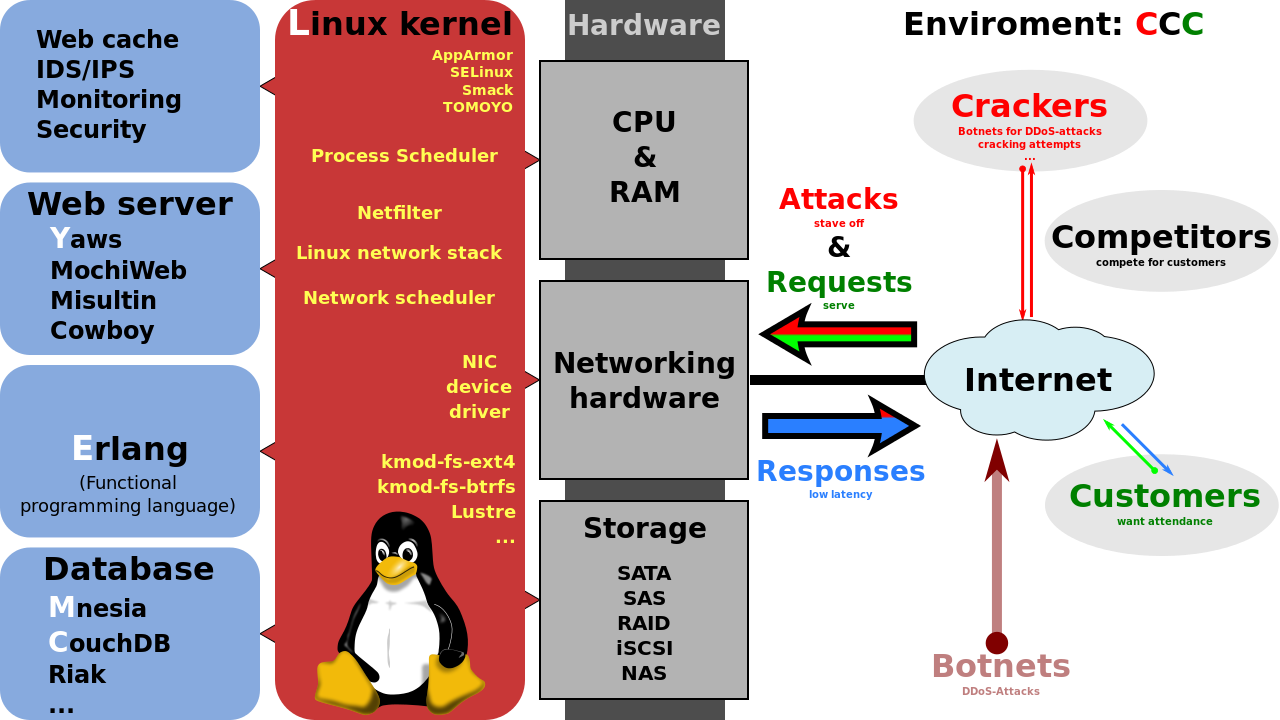
\includegraphics[scale=0.5]{LYME.png}
\caption{LYME}
\end{figure}




\section{Linux}


\begin{lstlisting}[language=bash]

\end{lstlisting}




\begin{lstlisting}[language=bash]

\end{lstlisting}


\section{Yaws}


\begin{lstlisting}[language=bash]

\end{lstlisting}




\begin{lstlisting}[language=bash]

\end{lstlisting}


\section{Mnesia}



\begin{lstlisting}[language=bash]

\end{lstlisting}



\begin{lstlisting}[language=bash]

\end{lstlisting}



\begin{lstlisting}[language=bash]

\end{lstlisting}


\section{Erlang}


\begin{lstlisting}[language=bash]

\end{lstlisting}




\begin{lstlisting}[language=bash]

\end{lstlisting}


\chapter{LAPP}



\section{Linux}


\begin{lstlisting}[language=bash]

\end{lstlisting}




\begin{lstlisting}[language=bash]

\end{lstlisting}


\section{Apache}


\begin{lstlisting}[language=bash]

\end{lstlisting}





\begin{lstlisting}[language=bash]

\end{lstlisting}

\section{PHP}


\begin{lstlisting}[language=bash]

\end{lstlisting}




\begin{lstlisting}[language=bash]

\end{lstlisting}


\section{PostgreSQL}


\begin{lstlisting}[language=bash]

\end{lstlisting}




\begin{lstlisting}[language=bash]

\end{lstlisting}




\begin{lstlisting}[language=bash]

\end{lstlisting}


\chapter{WAMP}



\section{Windows}


\begin{lstlisting}[language=bash]

\end{lstlisting}




\begin{lstlisting}[language=bash]

\end{lstlisting}



\section{Apache}


\begin{lstlisting}[language=bash]

\end{lstlisting}



\begin{lstlisting}[language=bash]

\end{lstlisting}


\section{MySQL}


\begin{lstlisting}[language=bash]

\end{lstlisting}




\begin{lstlisting}[language=bash]

\end{lstlisting}


\section{PHP}


\begin{lstlisting}[language=bash]

\end{lstlisting}




\begin{lstlisting}[language=bash]

\end{lstlisting}




\begin{lstlisting}[language=bash]

\end{lstlisting}

\chapter{LAMJ}



\section{Linux}



\begin{lstlisting}[language=bash]

\end{lstlisting}





\begin{lstlisting}[language=bash]

\end{lstlisting}

\section{Apache}


\begin{lstlisting}[language=bash]

\end{lstlisting}




\begin{lstlisting}[language=bash]

\end{lstlisting}


\section{MySQL}


\begin{lstlisting}[language=bash]

\end{lstlisting}




\begin{lstlisting}[language=bash]

\end{lstlisting}


\section{Java}



\begin{lstlisting}[language=bash]

\end{lstlisting}




\begin{lstlisting}[language=bash]

\end{lstlisting}


\chapter{BAMP}



\section{BSD}


\begin{lstlisting}[language=bash]

\end{lstlisting}





\begin{lstlisting}[language=bash]

\end{lstlisting}



\begin{lstlisting}[language=bash]

\end{lstlisting}



\section{Apache}




\begin{lstlisting}[language=bash]

\end{lstlisting}



\begin{lstlisting}[language=bash]

\end{lstlisting}



\section{MySQL}


\begin{lstlisting}[language=bash]

\end{lstlisting}



\begin{lstlisting}[language=bash]

\end{lstlisting}



\section{PHP}


\begin{lstlisting}[language=bash]

\end{lstlisting}



\begin{lstlisting}[language=bash]

\end{lstlisting}


\chapter{WIMP}



\section{Windows}



\begin{lstlisting}[language=bash]

\end{lstlisting}



\begin{lstlisting}[language=bash]

\end{lstlisting}


\section{IIS}



\begin{lstlisting}[language=bash]

\end{lstlisting}



\begin{lstlisting}[language=bash]

\end{lstlisting}


\section{MySQL}



\begin{lstlisting}[language=bash]

\end{lstlisting}



\begin{lstlisting}[language=bash]

\end{lstlisting}


\section{PHP}



\begin{lstlisting}[language=bash]

\end{lstlisting}



\begin{lstlisting}[language=bash]

\end{lstlisting}





\begin{lstlisting}[language=bash]

\end{lstlisting}



\begin{lstlisting}[language=bash]

\end{lstlisting}





\begin{lstlisting}[language=bash]

\end{lstlisting}



\begin{lstlisting}[language=bash]

\end{lstlisting}






\begin{lstlisting}[language=bash]

\end{lstlisting}



\begin{lstlisting}[language=bash]

\end{lstlisting}





\begin{lstlisting}[language=bash]

\end{lstlisting}



\begin{lstlisting}[language=bash]

\end{lstlisting}






\begin{lstlisting}[language=bash]

\end{lstlisting}



\begin{lstlisting}[language=bash]

\end{lstlisting}





\begin{lstlisting}[language=bash]

\end{lstlisting}



\begin{lstlisting}[language=bash]

\end{lstlisting}





\begin{lstlisting}[language=bash]

\end{lstlisting}



\begin{lstlisting}[language=bash]

\end{lstlisting}





\begin{lstlisting}[language=bash]

\end{lstlisting}



\begin{lstlisting}[language=bash]

\end{lstlisting}